%!TEX TS-program = xelatex
%!TEX encoding = UTF-8 Unicode
\documentclass[a4paper,12pt]{report}

% Basic packages
% \usepackage[utf8]{inputenc}  % Not needed with XeLaTeX
% \usepackage[T1]{fontenc}     % Not needed with XeLaTeX
\usepackage{fontspec}          % Required for XeLaTeX
\usepackage[french]{babel}
\usepackage{geometry}
\usepackage{graphicx}
\usepackage{fancyhdr}
\usepackage{listings}
\usepackage{xcolor}
\usepackage{titlesec}
\usepackage{enumitem}
\usepackage{booktabs}
\usepackage{float}
\usepackage{caption}
\usepackage{subcaption}
\usepackage{url}
\usepackage{tabularx}
\usepackage{setspace}

% Page geometry - reduced margins to save space
\geometry{top=2cm,bottom=2cm,right=2cm,left=2cm,headheight=15.5pt}

% Reduce spacing between paragraphs and lists
\setlength{\parskip}{0.5ex plus 0.1ex minus 0.1ex}
\setlength{\parindent}{1em}

% Make lists more compact
\setlist{noitemsep,topsep=2pt,parsep=0pt,partopsep=0pt}

% Reduce caption spacing
\captionsetup{font=small,skip=3pt}

% Reduce table row height
\renewcommand{\arraystretch}{0.9}

% Graphics path
\graphicspath{{images/}{images_pfe/}{screenshots/}}

% JavaScript language definition for listings
\lstdefinelanguage{JavaScript}{
  keywords={break, case, catch, continue, debugger, default, delete, do, else, false, finally, for, function, if, in, instanceof, new, null, return, switch, this, throw, true, try, typeof, var, void, while, with, let, const, class, export, import, from, async, await},
  morecomment=[l]{//},
  morecomment=[s]{/*}{*/},
  morestring=[b]',
  morestring=[b]",
  morestring=[b]`
}

% Code listings setup
\definecolor{codegreen}{rgb}{0,0.6,0}
\definecolor{codegray}{rgb}{0.5,0.5,0.5}
\definecolor{codepurple}{rgb}{0.58,0,0.82}
\definecolor{backcolour}{rgb}{0.95,0.95,0.95}

\lstdefinestyle{mystyle}{
    backgroundcolor=\color{backcolour},   
    commentstyle=\color{codegreen},
    keywordstyle=\color{magenta},
    numberstyle=\tiny\color{codegray},
    stringstyle=\color{codepurple},
    basicstyle=\ttfamily\footnotesize,
    breakatwhitespace=false,         
    breaklines=true,                 
    captionpos=b,                    
    keepspaces=true,                 
    numbers=left,                    
    numbersep=5pt,                  
    showspaces=false,                
    showstringspaces=false,
    showtabs=false,                  
    tabsize=2
}

\lstset{style=mystyle}

% Custom header and footer
\pagestyle{fancy}
\fancyhf{}
\fancyhead[L]{\leftmark}
\fancyhead[R]{\thepage}
\fancyfoot[C]{Système d'Enchères Automobiles}

% Customize chapter style - reduced spacing
\titleformat{\chapter}[display]
  {\normalfont\Large\bfseries}
  {\chaptertitlename\ \thechapter}{15pt}{\Large}
\titlespacing*{\chapter}{0pt}{30pt}{20pt}

% Make sections more compact
\titleformat{\section}
  {\normalfont\large\bfseries}
  {\thesection}{0.5em}{}
\titlespacing*{\section}{0pt}{2.0ex plus 0.5ex minus 0.1ex}{1.0ex plus 0.1ex}

\titleformat{\subsection}
  {\normalfont\normalsize\bfseries}
  {\thesubsection}{0.5em}{}
\titlespacing*{\subsection}{0pt}{1.5ex plus 0.5ex minus 0.1ex}{0.8ex plus 0.1ex}

% Bibliography setup
\usepackage[
    backend=biber,
    style=numeric,
    sorting=ynt
]{biblatex}
\addbibresource{references/references.bib}

% Make sure hyperref is loaded last
\usepackage{hyperref}
\hypersetup{
    colorlinks=true,
    linkcolor=black,
    filecolor=black,
    urlcolor=blue,
    citecolor=blue,
    pdftitle={Système d'Enchères Automobiles},
    pdfauthor={Auteur},
    pdfkeywords={enchères, automobile, application mobile, temps réel},
    pdfcreator={LaTeX},
    pdfproducer={XeLaTeX}
}

\begin{document}

\begin{titlepage}
    \centering
    \vspace*{1cm}
    {\Huge\bfseries Système d'Enchères Automobiles\par}
    \vspace{1.5cm}
    {\Large Conception et Implémentation d'une Application Mobile en Temps Réel\par}
    \vspace{2cm}
    {\Large Rapport de Projet\par}
    \vspace{3cm}
    {\Large\itshape Auteur\par}
    \vspace{3cm}
    {\large \today\par}
\end{titlepage}

\pagenumbering{Roman}

\chapter*{Dédicaces}

\vspace{2cm}

\begin{center}
\Large{Je dédie ce travail}
\end{center}

\vspace{1cm}

À mes chers parents,\\
Pour leur soutien inconditionnel et leurs encouragements constants tout au long de mes études.

\vspace{0.5cm}

À ma famille,\\
Pour leur présence et leur support moral dans tous mes projets.

\vspace{0.5cm}

À mes professeurs,\\
Pour leur dévouement et la qualité de leur enseignement.

\vspace{0.5cm}

À mes amis et collègues,\\
Pour leur aide et leur collaboration précieuse.

\vspace{0.5cm}

À tous ceux qui ont contribué de près ou de loin à ma formation et à la réalisation de ce projet. 
\chapter*{Remerciements}

\vspace{1cm}

Je tiens à exprimer ma profonde gratitude à toutes les personnes qui ont contribué à la réalisation de ce projet de fin d'études.

\vspace{0.5cm}

Mes remerciements s'adressent particulièrement à :

\vspace{0.5cm}

\textbf{Mon encadrant},\\
Pour son suivi régulier, ses conseils précieux et sa disponibilité tout au long de ce projet.

\vspace{0.5cm}

\textbf{L'équipe pédagogique},\\
Pour la qualité de la formation dispensée et leur engagement dans notre réussite.

\vspace{0.5cm}

\textbf{Les membres du jury},\\
Pour l'intérêt qu'ils portent à ce travail et le temps qu'ils consacrent à son évaluation.

\vspace{0.5cm}

\textbf{Mes collègues de promotion},\\
Pour leur esprit d'entraide et les moments de collaboration enrichissants.

\vspace{0.5cm}

Un remerciement spécial à tous ceux qui m'ont aidé à surmonter les défis techniques, notamment dans :
\begin{itemize}
    \item La résolution des problèmes de ports et de configuration
    \item La mise en place du système de mise à jour automatique des enchères
    \item L'optimisation des performances de l'application
    \item L'implémentation des fonctionnalités en temps réel
\end{itemize}

\vspace{0.5cm}

Enfin, je remercie ma famille pour leur soutien moral et leurs encouragements constants durant toute la période de réalisation de ce projet. 
\chapter*{Résumé}
Ce projet consiste en le développement d'une application d'enchères automobiles en temps réel utilisant React Native pour le frontend mobile, React.js pour le tableau de bord administratif, et Node.js avec MongoDB pour le backend. L'application permet aux utilisateurs de participer à des enchères de voitures, de placer des offres en temps réel, et de suivre leurs enchères gagnées ou perdues. Le système comprend également une interface d'administration pour la gestion des enchères, des utilisateurs et des véhicules.

Les principales fonctionnalités incluent :
\begin{itemize}
    \item Gestion automatique des statuts d'enchères
    \item Notifications en temps réel via Socket.IO
    \item Interface mobile native pour iOS
    \item Tableau de bord administratif complet
    \item Base de données MongoDB pour la persistance des données
\end{itemize}

\vspace{0.5cm}
\textbf{Mots clés:} Enchères en temps réel, React Native, Node.js, MongoDB, Socket.IO, Application mobile

\chapter*{Abstract}
This project involves the development of a real-time car auction application using React Native for the mobile frontend, React.js for the admin dashboard, and Node.js with MongoDB for the backend. The application allows users to participate in car auctions, place real-time bids, and track their won or lost auctions. The system also includes an administration interface for managing auctions, users, and vehicles.

Key features include:
\begin{itemize}
    \item Automatic auction status management
    \item Real-time notifications via Socket.IO
    \item Native iOS mobile interface
    \item Comprehensive admin dashboard
    \item MongoDB database for data persistence
\end{itemize}

\vspace{0.5cm}
\textbf{Keywords:} Real-time auctions, React Native, Node.js, MongoDB, Socket.IO, Mobile application 

\tableofcontents
\listoffigures
\listoftables
\clearpage

\pagenumbering{arabic}

\chapter{Introduction}

\section{Contexte et Motivation}

Le marché des ventes de véhicules d'occasion connaît une transformation numérique significative, avec une demande croissante pour des plateformes permettant d'acheter et de vendre des véhicules en ligne. Cette évolution est d'autant plus marquée que les consommateurs recherchent aujourd'hui des expériences d'achat plus accessibles, transparentes et efficaces.

Dans ce contexte, les systèmes d'enchères en ligne pour automobiles représentent une solution particulièrement adaptée, offrant un mécanisme de marché dynamique où la valeur des véhicules est déterminée collectivement par les acheteurs potentiels. Contrairement aux plateformes traditionnelles d'annonces automobiles, les systèmes d'enchères permettent une valorisation plus précise des véhicules et offrent une expérience interactive engageante pour les participants.

Cependant, la mise en œuvre d'un tel système présente des défis techniques considérables, notamment en termes de gestion des transactions en temps réel, de sécurisation des échanges, et de conception d'interfaces utilisateur intuitives sur appareils mobiles. Ces défis constituent le point de départ de notre projet.

\section{Problématique}

Le développement d'une application d'enchères automobiles en temps réel soulève plusieurs questions essentielles:

\begin{itemize}
    \item Comment concevoir un système d'enchères qui garantit l'équité et la transparence pour tous les participants?
    \item Quelles architectures techniques permettent de gérer efficacement la concurrence et le temps réel dans un contexte d'enchères?
    \item Comment assurer une expérience utilisateur fluide et accessible sur plateformes mobiles, malgré les contraintes de connectivité et les variations de performances des appareils?
    \item Quels mécanismes de sécurité mettre en place pour protéger les transactions et les données personnelles des utilisateurs?
    \item Comment structurer l'application pour qu'elle puisse évoluer et s'adapter aux besoins futurs du marché?
\end{itemize}

Ces problématiques constituent le cœur de notre réflexion et ont guidé les choix techniques et fonctionnels tout au long du développement de l'application.

\section{Objectifs du Projet}

Dans le cadre de ce projet, nous nous sommes fixé plusieurs objectifs:

\subsection{Objectifs Fonctionnels}

\begin{itemize}
    \item Développer une application mobile permettant aux utilisateurs de consulter et participer à des enchères automobiles
    \item Mettre en place un système d'enchères en temps réel avec mise à jour instantanée des prix
    \item Implémenter des mécanismes de notification pour informer les utilisateurs des événements importants (surenchère, fin d'enchère, etc.)
    \item Créer un panneau d'administration pour la gestion des véhicules, des enchères et des utilisateurs
    \item Assurer une présentation détaillée et attrayante des véhicules mis aux enchères
\end{itemize}

\subsection{Objectifs Techniques}

\begin{itemize}
    \item Concevoir une architecture évolutive et maintenable basée sur des technologies modernes
    \item Implémenter des communications bidirectionnelles en temps réel entre clients et serveur
    \item Garantir la sécurité et l'intégrité des données dans un environnement d'enchères concurrentiel
    \item Optimiser les performances pour assurer une expérience fluide, même lors de pics d'activité
    \item Développer une interface utilisateur réactive et intuitive sur plateformes iOS et Android
\end{itemize}

\subsection{Objectifs Pédagogiques}

\begin{itemize}
    \item Approfondir la maîtrise du développement d'applications mobiles avec React Native
    \item Explorer les techniques de communication en temps réel avec Socket.io
    \item Appliquer les principes de conception UML à un projet concret
    \item Développer des compétences en architecture de systèmes distribués
    \item Mettre en pratique les méthodes de gestion de projet agile
\end{itemize}

\section{Périmètre du Projet}

\subsection{Fonctionnalités Couvertes}

Le projet couvre les fonctionnalités suivantes:

\begin{itemize}
    \item Inscription et authentification des utilisateurs
    \item Consultation des enchères en cours et à venir
    \item Participation aux enchères avec mise à jour en temps réel
    \item Système de notifications pour les événements importants
    \item Gestion de profil utilisateur
    \item Interface d'administration pour la gestion des enchères et des véhicules
    \item Visualisation détaillée des véhicules avec galerie d'images
    \item Historique des enchères et des transactions
\end{itemize}

\subsection{Limites et Exclusions}

Le projet n'inclut pas:

\begin{itemize}
    \item Le traitement des paiements en ligne (prévu pour une version ultérieure)
    \item L'intégration avec des services de vérification d'historique de véhicules
    \item La gestion logistique de livraison des véhicules
    \item Un système de messagerie instantanée entre acheteurs et vendeurs
    \item Une version web desktop complète (focus sur applications mobiles)
\end{itemize}

\section{Méthodologie}

\subsection{Approche de Développement}

Le projet a été mené selon une approche agile, avec:

\begin{itemize}
    \item Des sprints de deux semaines
    \item Des réunions quotidiennes pour synchroniser l'équipe
    \item Des revues de sprint pour valider les fonctionnalités développées
    \item Une amélioration continue basée sur les retours des tests utilisateurs
\end{itemize}

\subsection{Phases du Projet}

Le projet s'est déroulé en plusieurs phases:

\begin{enumerate}
    \item \textbf{Analyse des besoins}: Identification des exigences fonctionnelles et techniques
    \item \textbf{Conception}: Élaboration de l'architecture et modélisation UML
    \item \textbf{Développement}: Implémentation itérative des fonctionnalités
    \item \textbf{Tests}: Validation technique et fonctionnelle
    \item \textbf{Déploiement}: Mise en production de l'application
    \item \textbf{Maintenance}: Correction des bugs et améliorations continues
\end{enumerate}

\subsection{Outils de Gestion}

Pour la gestion du projet, nous avons utilisé:

\begin{itemize}
    \item \textbf{Jira}: Suivi des tâches et des sprints
    \item \textbf{GitHub}: Gestion de versions et revue de code
    \item \textbf{Figma}: Conception des interfaces utilisateur
    \item \textbf{Lucidchart}: Création des diagrammes UML
    \item \textbf{Slack}: Communication d'équipe
\end{itemize}

\section{Structure du Rapport}

Ce rapport est organisé en plusieurs chapitres qui couvrent l'ensemble du processus de développement:

\begin{description}
    \item[Chapitre 1-4] Introduction, remerciements et résumé.
    \item[Chapitre 5] Introduction générale au projet.
    \item[Chapitre 6] Présentation détaillée des technologies et outils utilisés.
    \item[Chapitre 7] Manuel d'utilisation de l'application.
    \item[Chapitre 8] Analyse des besoins et des exigences du système.
    \item[Chapitre 9] Conception du système avec diagrammes UML.
    \item[Chapitre 10] Implémentation technique et détails de réalisation.
    \item[Chapitre 11] Défis d'implémentation et perspectives d'évolution.
    \item[Chapitre 12] Conclusion et bilan du projet.
\end{description}

Chaque chapitre vise à présenter de manière claire et structurée les différents aspects du développement de notre application d'enchères automobiles, depuis l'analyse initiale jusqu'à la mise en production et aux perspectives futures.

\section{Aperçu de l'Application}

Notre application d'enchères automobiles se distingue par plusieurs caractéristiques clés:

\begin{itemize}
    \item Une interface utilisateur moderne et intuitive, optimisée pour les appareils mobiles
    \item Un système d'enchères en temps réel permettant une expérience interactive
    \item Une architecture technique robuste basée sur des technologies éprouvées
    \item Une attention particulière à la sécurité et à la protection des données
    \item Une conception évolutive permettant l'ajout futur de fonctionnalités
\end{itemize}

Ces caractéristiques constituent les fondements de notre solution et seront détaillées dans les chapitres suivants, accompagnées d'illustrations, de diagrammes et d'exemples de code. 
\chapter{État de l'Art}

\section{Introduction aux Systèmes d'Enchères en Ligne}

Les enchères en ligne ont considérablement évolué depuis leur apparition dans les années 1990. Ce qui a commencé comme de simples plateformes de vente aux enchères s'est transformé en écosystèmes sophistiqués intégrant des technologies avancées pour améliorer l'expérience utilisateur, la sécurité des transactions et l'efficacité globale du processus d'enchère.

\subsection{Évolution Historique}

L'histoire des enchères en ligne peut être divisée en plusieurs phases distinctes:

\begin{enumerate}
    \item \textbf{Première génération (1995-2000)}: Caractérisée par des plateformes comme eBay, offrant des fonctionnalités basiques d'enchères avec des interfaces utilisateur simples et des mécanismes de communication asynchrones.
    
    \item \textbf{Deuxième génération (2000-2010)}: Introduction de fonctionnalités avancées comme les enchères automatiques, les systèmes de réputation, et l'intégration de moyens de paiement sécurisés.
    
    \item \textbf{Troisième génération (2010-2015)}: Développement de plateformes spécialisées par secteur (art, automobiles, immobilier), avec des fonctionnalités adaptées aux spécificités de chaque domaine.
    
    \item \textbf{Quatrième génération (2015-présent)}: Intégration de technologies temps réel, d'applications mobiles avancées, d'intelligence artificielle, et de mécanismes de vérification d'identité renforcés.
\end{enumerate}

\subsection{Typologies d'Enchères}

Les systèmes d'enchères en ligne peuvent implémenter différents modèles d'enchères, chacun avec ses propres règles et mécanismes:

\begin{itemize}
    \item \textbf{Enchères anglaises}: Le modèle le plus courant, où les participants enchérissent à la hausse jusqu'à ce que plus personne ne surenchérisse.
    
    \item \textbf{Enchères hollandaises}: Commençant à un prix élevé qui diminue progressivement jusqu'à ce qu'un acheteur accepte le prix courant.
    
    \item \textbf{Enchères à prix secret}: Les participants soumettent leurs offres en privé, et le plus offrant remporte l'enchère.
    
    \item \textbf{Enchères à paliers}: Le prix augmente par incréments prédéfinis à intervalles réguliers.
    
    \item \textbf{Enchères inversées}: Les vendeurs enchérissent à la baisse pour offrir le prix le plus bas pour un service ou produit.
\end{itemize}

Notre système d'enchères automobiles s'appuie principalement sur le modèle d'enchères anglaises, tout en intégrant certaines fonctionnalités avancées comme l'extension automatique du temps lors d'enchères de dernière minute.

\section{Analyse des Plateformes d'Enchères Automobiles Existantes}

Plusieurs plateformes d'enchères automobiles existantes ont été analysées pour identifier les meilleures pratiques et les opportunités d'innovation.

\subsection{Acteurs Majeurs du Marché}

\begin{description}
    \item[Bring a Trailer] Plateforme spécialisée dans les véhicules de collection et d'enthousiaste, caractérisée par des descriptions détaillées, une communauté active et un modèle d'enchères de 7 jours avec extension automatique.
    
    \item[Cars \& Bids] Focalisée sur les véhicules modernes enthousiastes (moins de 30 ans), avec une interface utilisateur moderne, des frais réduits, et une vérification des annonces.
    
    \item[eBay Motors] Plateforme généraliste avec une section dédiée aux véhicules, offrant à la fois des options d'achat immédiat et d'enchères, avec une large audience mondiale.

    \item[Copart] Spécialisée dans les véhicules accidentés et de récupération, avec un système d'enchères hybride (en personne et en ligne) destiné principalement aux professionnels.
    
    \item[CarOnSale] Plateforme européenne dédiée aux professionnels de l'automobile, avec un système d'enchères B2B et des services d'inspection des véhicules.
\end{description}

\subsection{Analyse Comparative}

\begin{table}[h]
\centering
\begin{tabular}{|p{2.5cm}|p{2cm}|p{2cm}|p{2cm}|p{2cm}|p{2cm}|}
\hline
\textbf{Caractéristique} & \textbf{Bring a Trailer} & \textbf{Cars \& Bids} & \textbf{eBay Motors} & \textbf{Copart} & \textbf{CarOnSale} \\
\hline
Public cible & Collectionneurs & Enthousiastes modernes & Grand public & Professionnels & Professionnels \\
\hline
Durée d'enchère & 7 jours & 7 jours & Variable & Court terme & 24-48h \\
\hline
Extension auto. & Oui & Oui & Non & Limitée & Oui \\
\hline
Mobile App & Limitée & Oui & Complète & Complète & Basique \\
\hline
Communication TR & Modérée & Avancée & Limitée & Basique & Modérée \\
\hline
Inspection & Par la communauté & Vérification photos & Optionnelle & Complète & Standardisée \\
\hline
Modèle de revenus & Commission vendeur et acheteur & Commission vendeur & Commission vendeur & Frais d'inscription et commission & Commission variable \\
\hline
\end{tabular}
\caption{Comparaison des principales plateformes d'enchères automobiles}
\label{table:platform-comparison}
\end{table}

Cette analyse comparative révèle plusieurs tendances et opportunités:

\begin{itemize}
    \item L'importance croissante des fonctionnalités mobiles complètes
    \item La valeur ajoutée des communications en temps réel pendant les enchères
    \item L'évolution vers des systèmes d'extension automatique pour éviter le "sniping" (enchères de dernière seconde)
    \item Le besoin d'équilibrer la simplicité d'utilisation et la richesse fonctionnelle
\end{itemize}

\section{Technologies Clés pour les Systèmes d'Enchères Modernes}

Le développement d'un système d'enchères automobiles moderne nécessite l'intégration de plusieurs technologies avancées.

\subsection{Technologies Frontend}

\subsubsection{Applications Mobiles Natives vs Hybrides}

Le débat entre applications natives et hybrides reste pertinent pour les plateformes d'enchères:

\begin{itemize}
    \item \textbf{Applications natives}: Offrent des performances optimales et un accès complet aux fonctionnalités du dispositif, mais nécessitent un développement séparé pour chaque plateforme.
    
    \item \textbf{Applications hybrides}: Permettent un développement unique pour plusieurs plateformes, avec des performances qui se sont considérablement améliorées grâce à des frameworks comme React Native et Flutter.
\end{itemize}

Pour notre système, nous avons opté pour React Native, qui offre un bon compromis entre performances natives et efficacité de développement multiplateforme.

\subsubsection{Interfaces Utilisateur Réactives}

Les tendances modernes en matière d'interface utilisateur pour les systèmes d'enchères incluent:

\begin{itemize}
    \item \textbf{Design minimaliste}: Interfaces épurées qui mettent l'accent sur le contenu et les fonctionnalités essentielles.
    
    \item \textbf{Navigation intuitive}: Structures de navigation simples et cohérentes qui facilitent l'accès aux différentes fonctionnalités.
    
    \item \textbf{Retours visuels immédiats}: Animations et transitions subtiles qui fournissent un feedback instantané aux actions de l'utilisateur.
    
    \item \textbf{Microinteractions}: Petites animations fonctionnelles qui enrichissent l'expérience utilisateur, particulièrement importantes dans le contexte des enchères où chaque interaction peut être critique.
\end{itemize}

\subsection{Technologies Backend}

\subsubsection{Architectures API}

Plusieurs approches architecturales sont utilisées dans les systèmes d'enchères modernes:

\begin{itemize}
    \item \textbf{REST}: Architecture mature et largement adoptée, bien adaptée pour les opérations CRUD standard.
    
    \item \textbf{GraphQL}: Offre une flexibilité accrue pour les requêtes complexes et réduit le sur-fetching, particulièrement utile pour les applications mobiles avec des contraintes de bande passante.
    
    \item \textbf{gRPC}: Protocole haute performance utilisant Protocol Buffers, adapté pour les communications entre microservices.
\end{itemize}

Notre système utilise principalement une API RESTful pour sa simplicité et sa large compatibilité, tout en intégrant des WebSockets pour les communications en temps réel.

\subsubsection{Communication Temps Réel}

Les technologies de communication temps réel sont essentielles pour les systèmes d'enchères:

\begin{itemize}
    \item \textbf{WebSockets}: Protocole établissant une connexion bidirectionnelle persistante entre le client et le serveur, idéal pour les mises à jour d'enchères en temps réel.
    
    \item \textbf{Server-Sent Events (SSE)}: Alternative plus légère aux WebSockets, adaptée pour les scénarios où la communication est principalement du serveur vers le client.
    
    \item \textbf{Socket.IO}: Bibliothèque qui simplifie l'utilisation des WebSockets avec des fonctionnalités de fallback et de reconnexion automatique.
\end{itemize}

Notre choix s'est porté sur Socket.IO pour sa robustesse, sa facilité d'intégration et ses mécanismes de fallback qui garantissent une expérience utilisateur optimale même dans des conditions réseau variables.

\subsection{Technologies de Base de Données}

\subsubsection{Bases de Données SQL vs NoSQL}

Le choix entre SQL et NoSQL dépend des besoins spécifiques du système:

\begin{itemize}
    \item \textbf{SQL}: Offre des garanties ACID fortes et une structure relationnelle bien adaptée pour les données structurées avec des relations complexes.
    
    \item \textbf{NoSQL}: Propose une meilleure scalabilité horizontale et une flexibilité de schéma adaptée aux données semi-structurées et aux évolutions rapides.
\end{itemize}

Les systèmes d'enchères modernes utilisent souvent une approche hybride, avec:

\begin{itemize}
    \item Des bases SQL pour les données critiques nécessitant une intégrité forte (transactions, informations utilisateurs)
    \item Des bases NoSQL pour les données à haute vélocité ou nécessitant une évolutivité particulière (historique des enchères, logs d'activité)
\end{itemize}

Notre système utilise MongoDB comme solution principale, complétée par Redis pour le caching et la gestion des sessions.

\subsubsection{Technologies de Cache}

Les mécanismes de cache sont cruciaux pour maintenir les performances sous charge:

\begin{itemize}
    \item \textbf{Redis}: Solution de stockage en mémoire polyvalente, utilisée pour le caching, les sessions, et les files d'attente de messages.
    
    \item \textbf{Memcached}: Alternative plus simple et focalisée uniquement sur le caching.
    
    \item \textbf{CDN}: Pour la distribution optimisée des assets statiques comme les images de véhicules.
\end{itemize}

\section{Sécurité et Authentification}

\subsection{Mécanismes d'Authentification Modernes}

Les systèmes d'enchères nécessitent des mécanismes d'authentification robustes:

\begin{itemize}
    \item \textbf{JWT (JSON Web Tokens)}: Standard moderne pour l'authentification sans état, bien adapté aux architectures distribuées.
    
    \item \textbf{OAuth 2.0 / OpenID Connect}: Protocoles standardisés pour l'authentification déléguée et la fédération d'identité.
    
    \item \textbf{Authentification Multi-facteurs}: Couche de sécurité supplémentaire devenue standard pour les plateformes manipulant des transactions financières.
    
    \item \textbf{Authentification biométrique}: Intégration des capteurs d'empreintes digitales et de reconnaissance faciale des appareils mobiles.
\end{itemize}

\subsection{Sécurisation des Transactions}

La sécurité des transactions est particulièrement critique dans les systèmes d'enchères automobiles:

\begin{itemize}
    \item \textbf{Validation stricte des enchères}: Vérifications côté serveur pour prévenir les manipulations.
    
    \item \textbf{Prévention des conditions de course}: Mécanismes de verrouillage et transactions atomiques pour garantir l'intégrité des enchères concurrentes.
    
    \item \textbf{Audit trails}: Journalisation immuable de toutes les actions critiques pour la traçabilité et la résolution de litiges.
    
    \item \textbf{Chiffrement de bout en bout}: Protection des communications sensibles entre l'utilisateur et le serveur.
    
    \item \textbf{Détection de fraude}: Algorithmes de détection d'anomalies pour identifier les comportements suspects.
\end{itemize}

\section{Tendances Émergentes et Innovations}

\subsection{Intelligence Artificielle et Machine Learning}

L'IA et le ML transforment plusieurs aspects des systèmes d'enchères:

\begin{itemize}
    \item \textbf{Estimation automatique de valeur}: Algorithmes prédictifs pour suggérer des prix de départ optimaux basés sur les caractéristiques du véhicule et les données historiques.
    
    \item \textbf{Détection de fraude avancée}: Modèles de ML pour identifier les schémas d'activités suspectes en temps réel.
    
    \item \textbf{Recommandations personnalisées}: Suggestion de véhicules pertinents basée sur l'historique et les préférences de l'utilisateur.
    
    \item \textbf{Analyse d'images}: Validation automatique des photos de véhicules et détection des défauts ou incohérences.
\end{itemize}

\subsection{Blockchain et Contrats Intelligents}

La technologie blockchain offre des perspectives intéressantes pour les systèmes d'enchères:

\begin{itemize}
    \item \textbf{Transparence et immuabilité}: Enregistrement inaltérable de l'historique des enchères et des transactions.
    
    \item \textbf{Contrats intelligents}: Automatisation des règles d'enchères et des processus post-enchère (paiement, transfert de propriété).
    
    \item \textbf{Tokenisation}: Représentation numérique de la propriété d'un véhicule facilitant les transferts sécurisés.
    
    \item \textbf{Vérification d'identité décentralisée}: Systèmes KYC (Know Your Customer) plus robustes et respectueux de la vie privée.
\end{itemize}

Bien que prometteuses, ces technologies restent émergentes dans le secteur des enchères automobiles et font face à des défis d'adoption liés à la complexité technique et aux questions réglementaires.

\subsection{Réalité Augmentée et Virtuelle}

Les technologies immersives commencent à être intégrées dans les plateformes d'enchères automobiles avancées:

\begin{itemize}
    \item \textbf{Visites virtuelles}: Exploration détaillée des véhicules en 3D sans nécessité de déplacement physique.
    
    \item \textbf{Superposition d'informations}: Utilisation de la RA pour afficher des informations contextuelles sur les différents éléments d'un véhicule.
    
    \item \textbf{Simulation de conduite}: Expériences virtuelles permettant d'avoir un aperçu du comportement routier d'un véhicule.
\end{itemize}

\section{Défis et Opportunités du Marché}

\subsection{Défis Actuels}

Le développement et l'exploitation de systèmes d'enchères automobiles font face à plusieurs défis:

\begin{itemize}
    \item \textbf{Confiance et vérification}: Établir la confiance dans un environnement en ligne où l'acheteur ne peut pas inspecter physiquement le véhicule.
    
    \item \textbf{Réglementation}: Navigation dans un paysage réglementaire complexe et variable selon les juridictions.
    
    \item \textbf{Concurrence}: Différenciation dans un marché de plus en plus saturé.
    
    \item \textbf{Expérience mobile}: Offrir une expérience d'enchère complète et fluide sur des appareils mobiles malgré les limitations d'interface.
    
    \item \textbf{Internationalisation}: Adaptation aux spécificités régionales tout en maintenant une plateforme cohérente.
\end{itemize}

\subsection{Opportunités de Marché}

Plusieurs tendances créent des opportunités significatives:

\begin{itemize}
    \item \textbf{Digitalisation accélérée}: Adoption croissante des solutions numériques pour l'achat et la vente de véhicules, accélérée par la pandémie de COVID-19.
    
    \item \textbf{Évolution des préférences consommateurs}: Augmentation de la confiance dans les achats en ligne de biens de valeur élevée.
    
    \item \textbf{Segment des véhicules électriques}: Croissance rapide créant de nouveaux segments de marché avec des besoins spécifiques.
    
    \item \textbf{Marchés émergents}: Expansion dans des régions où le commerce électronique automobile est encore en développement.
    
    \item \textbf{Services complémentaires}: Intégration de services à valeur ajoutée (financement, assurance, logistique) dans l'écosystème d'enchères.
\end{itemize}

\section{Conclusion et Positionnement de Notre Solution}

L'analyse de l'état de l'art révèle un secteur des enchères automobiles en ligne en pleine évolution, avec une sophistication croissante des technologies et des attentes utilisateurs de plus en plus élevées.

Notre système d'enchères automobiles se positionne à l'intersection de ces tendances, avec:

\begin{itemize}
    \item Une approche centrée sur l'expérience mobile, reflétant la transition vers un usage majoritairement mobile
    \item Un système de communication en temps réel optimisé, crucial pour l'engagement des utilisateurs
    \item Une architecture évolutive capable d'intégrer progressivement les innovations technologiques
    \item Un focus sur la transparence et la sécurité pour établir la confiance des utilisateurs
\end{itemize} 

Les choix technologiques et fonctionnels détaillés dans ce rapport s'inscrivent dans cette vision, visant à créer une plateforme qui répond aux besoins actuels tout en anticipant les évolutions futures du marché. 
\chapter{Technologies et Outils Utilisés}

\section{Vue d'Ensemble de la Stack Technologique}

Le développement d'une application d'enchères automobiles en temps réel nécessite une pile technologique robuste et moderne, capable de gérer efficacement les communications bidirectionnelles, le traitement des données et l'expérience utilisateur. Notre choix s'est porté sur un ensemble de technologies complémentaires formant un écosystème cohérent.

\subsection{Architecture Globale}

L'architecture technique du système repose sur quatre composants principaux:

\begin{itemize}
    \item \textbf{Frontend Mobile}: Interface utilisateur développée avec React Native
    \item \textbf{Backend API}: Serveur RESTful développé avec Node.js et Express
    \item \textbf{Communication Temps Réel}: Implémentée avec Socket.io
    \item \textbf{Base de Données}: MongoDB pour le stockage persistant des données
\end{itemize}

Cette architecture permet une séparation claire des responsabilités tout en assurant une communication fluide entre les différentes couches du système.

\section{Technologies Frontend}

\subsection{React Native}

React Native constitue le choix central pour le développement de l'interface utilisateur mobile. Cette technologie présente plusieurs avantages décisifs:

\begin{itemize}
    \item \textbf{Développement multiplateforme}: Une base de code unique déployable sur iOS et Android
    \item \textbf{Performances natives}: Rendu d'interfaces utilisateur natives, offrant des performances proches des applications développées en code natif
    \item \textbf{Architecture à composants}: Organisation modulaire du code favorisant la réutilisation et la maintenance
    \item \textbf{Hot Reloading}: Cycle de développement accéléré grâce au rechargement à chaud
    \item \textbf{Écosystème riche}: Large éventail de bibliothèques tierces disponibles
\end{itemize}

\subsubsection{Composants React Native Principaux}
L'application utilise intensivement les composants React Native suivants:

\begin{verbatim}
import React, { useState, useEffect } from 'react';
import {
  View,
  Text,
  Image,
  TouchableOpacity,
  FlatList,
  StyleSheet,
  ActivityIndicator,
  Alert
} from 'react-native';
\end{verbatim}

\subsection{React Navigation}

La navigation entre les écrans est gérée par React Navigation, qui offre:

\begin{itemize}
    \item Une navigation fluide et performante entre les écrans
    \item La gestion de l'historique de navigation
    \item Différents types de navigateurs (stack, tab, drawer)
    \item Une intégration profonde avec les gestes natifs
\end{itemize}

\begin{verbatim}
import { NavigationContainer } from '@react-navigation/native';
import { createStackNavigator } from '@react-navigation/stack';
import { createBottomTabNavigator } from '@react-navigation/bottom-tabs';

const Stack = createStackNavigator();
const Tab = createBottomTabNavigator();

// Configuration de base de la navigation
function AppNavigator() {
  return (
    <NavigationContainer>
      <Stack.Navigator initialRouteName="Home">
        <Stack.Screen
          name="Home"
          component={HomeScreen}
          options={{ 
            title: 'Accueil',
            headerStyle: styles.header
          }}
        />
        <Stack.Screen name="AuctionDetail" component={AuctionDetailScreen} />
        {/* Autres écrans... */}
      </Stack.Navigator>
    </NavigationContainer>
  );
}
\end{verbatim}

\subsection{Gestion de l'État}

La gestion de l'état de l'application utilise plusieurs approches complémentaires:

\begin{itemize}
    \item \textbf{Hooks React}: useState et useEffect pour l'état local des composants
    \item \textbf{Context API}: Pour le partage d'état entre composants proches
    \item \textbf{AsyncStorage}: Pour la persistance locale des données comme les tokens d'authentification
\end{itemize}

\begin{verbatim}
// Exemple d'utilisation du Context API pour l'authentification
const AuthContext = React.createContext();

export const AuthProvider = ({ children }) => {
  const [user, setUser] = useState(null);
  const [loading, setLoading] = useState(true);
  
  // Vérification du token au démarrage
  useEffect(() => {
    const loadUserFromStorage = async () => {
      try {
        const token = await AsyncStorage.getItem('userToken');
        if (token) {
          const userData = await authService.getUserData(token);
          setUser(userData);
        }
      } catch (error) {
        console.log('Failed to load user:', error);
      } finally {
        setLoading(false);
      }
    };
    
    loadUserFromStorage();
  }, []);
  
  // Fonctions d'authentification
  const login = async (email, password) => {
    setLoading(true);
    try {
      const response = await authService.login(email, password);
      await AsyncStorage.setItem('userToken', response.token);
      setUser(response.user);
      return { success: true };
    } catch (error) {
      return { success: false, error: error.message };
    } finally {
      setLoading(false);
    }
  };
  
  const logout = async () => {
    await AsyncStorage.removeItem('userToken');
    setUser(null);
  };
  
  // Valeur fournie par le contexte
  const authContextValue = {
    user,
    loading,
    login,
    logout,
    isAuthenticated: !!user
  };
  
  return (
    <AuthContext.Provider value={authContextValue}>
      {children}
    </AuthContext.Provider>
  );
};
\end{verbatim}

\subsection{Bibliothèques UI Complémentaires}

Pour enrichir l'interface utilisateur, plusieurs bibliothèques complémentaires sont utilisées:

\begin{itemize}
    \item \textbf{React Native Elements}: Composants UI pré-stylisés et personnalisables
    \item \textbf{React Native Vector Icons}: Collection d'icônes vectorielles
    \item \textbf{React Native Gesture Handler}: Gestion avancée des gestes tactiles
    \item \textbf{React Native Reanimated}: Animations fluides et performantes
\end{itemize}

\section{Technologies Backend}

\subsection{Node.js et Express}

Le backend est développé avec Node.js et Express, offrant:

\begin{itemize}
    \item \textbf{Architecture événementielle non-bloquante}: Idéale pour les applications en temps réel
    \item \textbf{Performance}: Traitement efficace des requêtes simultanées
    \item \textbf{Ecosystème npm}: Accès à un vaste répertoire de packages
    \item \textbf{JavaScript full-stack}: Uniformité du langage entre frontend et backend
\end{itemize}

\begin{verbatim}
const express = require('express');
const app = express();
const cors = require('cors');
const morgan = require('morgan');
const helmet = require('helmet');

// Middleware de base
app.use(cors());
app.use(express.json());
app.use(morgan('dev'));
app.use(helmet());

// Routes API
app.use('/api/auth', require('./routes/authRoutes'));
app.use('/api/auctions', require('./routes/auctionRoutes'));
app.use('/api/cars', require('./routes/carRoutes'));
app.use('/api/users', require('./routes/userRoutes'));

// Middleware de gestion d'erreurs
app.use((err, req, res, next) => {
  console.error(err.stack);
  res.status(500).json({ 
    message: 'Une erreur est survenue',
    error: process.env.NODE_ENV === 'production' ? {} : err
  });
});

// Démarrage du serveur
const PORT = process.env.PORT || 5000;
app.listen(PORT, () => {
  console.log(`Server running on port ${PORT}`);
});
\end{verbatim}

\subsection{Architecture API RESTful}

L'API backend suit les principes REST avec:

\begin{itemize}
    \item Organisation des endpoints par ressources
    \item Utilisation appropriée des méthodes HTTP (GET, POST, PUT, DELETE)
    \item Réponses structurées avec codes HTTP standards
    \item Pagination des résultats pour les listes volumineuses
\end{itemize}

\begin{verbatim}
// Exemple de contrôleur RESTful pour les enchères
const auctionController = {
  // GET /api/auctions
  getAll: async (req, res) => {
    try {
      const page = parseInt(req.query.page) || 1;
      const limit = parseInt(req.query.limit) || 10;
      const skip = (page - 1) * limit;
      
      const auctions = await Auction.find()
        .sort({ createdAt: -1 })
        .skip(skip)
        .limit(limit)
        .populate('car', 'brand model year images');
      
      const total = await Auction.countDocuments();
      
      res.json({
        data: auctions,
        meta: {
          total,
          page,
          lastPage: Math.ceil(total / limit)
        }
      });
    } catch (error) {
      res.status(500).json({ message: error.message });
    }
  },
  
  // GET /api/auctions/:id
  getById: async (req, res) => {
    try {
      const auction = await Auction.findById(req.params.id)
        .populate('car')
        .populate({
          path: 'bids',
          options: { sort: { amount: -1 } },
          populate: { path: 'user', select: 'username profileImage' }
        });
      
      if (!auction) {
        return res.status(404).json({ message: 'Enchère non trouvée' });
      }
      
      res.json(auction);
    } catch (error) {
      res.status(500).json({ message: error.message });
    }
  }
  
  // Autres méthodes...
};
\end{verbatim}

\subsection{Sécurité}

La sécurité du backend est assurée par plusieurs mécanismes:

\begin{itemize}
    \item \textbf{JSON Web Tokens (JWT)}: Pour l'authentification sécurisée
    \item \textbf{bcrypt}: Pour le hachage sécurisé des mots de passe
    \item \textbf{Helmet}: Protection contre les vulnérabilités web courantes
    \item \textbf{express-rate-limit}: Limitation du nombre de requêtes pour prévenir les attaques par force brute
    \item \textbf{express-validator}: Validation des entrées utilisateur
\end{itemize}

\begin{verbatim}
// Middleware d'authentification
const jwt = require('jsonwebtoken');
const User = require('../models/User');

const auth = async (req, res, next) => {
  try {
    const token = req.header('Authorization').replace('Bearer ', '');
    const decoded = jwt.verify(token, process.env.JWT_SECRET);
    const user = await User.findOne({ 
      _id: decoded.id,
      'tokens.token': token 
    });
    
    if (!user) {
      throw new Error();
    }
    
    req.token = token;
    req.user = user;
    next();
  } catch (error) {
    res.status(401).json({ message: 'Veuillez vous authentifier' });
  }
};
\end{verbatim}

\section{Communication Temps Réel avec Socket.io}

\subsection{Principes de Fonctionnement}

Socket.io est utilisé pour établir une communication bidirectionnelle en temps réel entre le client et le serveur, permettant:

\begin{itemize}
    \item Mise à jour instantanée des enchères
    \item Notifications en temps réel
    \item Actualisation du statut des enchères sans rechargement
    \item Support de la reconnexion automatique
\end{itemize}

\begin{verbatim}
// Configuration Socket.io côté serveur
const http = require('http');
const socketIo = require('socket.io');
const jwt = require('jsonwebtoken');

const server = http.createServer(app);
const io = socketIo(server, {
  cors: {
    origin: '*',
    methods: ['GET', 'POST']
  }
});

// Middleware d'authentification Socket.io
io.use((socket, next) => {
  if (socket.handshake.query && socket.handshake.query.token) {
    const token = socket.handshake.query.token;
    jwt.verify(token, process.env.JWT_SECRET, (err, decoded) => {
      if (err) return next(new Error('Authentication error'));
      socket.decoded = decoded;
      next();
    });
  } else {
    next(new Error('Authentication error'));
  }
});

// Gestion des événements Socket.io
io.on('connection', (socket) => {
  console.log('User connected:', socket.decoded.id);
  
  // Rejoindre une salle d'enchère spécifique
  socket.on('join_auction', (auctionId) => {
    socket.join(`auction_${auctionId}`);
    console.log(`User joined auction: ${auctionId}`);
  });
  
  // Soumettre une enchère
  socket.on('place_bid', async (data) => {
    try {
      const { auctionId, amount } = data;
      const userId = socket.decoded.id;
      
      // Traitement de l'enchère via le service
      const result = await auctionService.placeBid(auctionId, userId, amount);
      
      if (result.success) {
        // Diffuser la mise à jour à tous les participants
        io.to(`auction_${auctionId}`).emit('bid_update', {
          auctionId,
          newPrice: result.data.amount,
          bidder: result.data.bidderName,
          timestamp: new Date()
        });
        
        // Notifier l'enchérisseur précédent
        if (result.data.previousBidder) {
          io.to(`user_${result.data.previousBidder}`).emit('outbid', {
            auctionId,
            carName: result.data.carName
          });
        }
      } else {
        // Informer l'utilisateur de l'échec
        socket.emit('bid_error', {
          auctionId,
          message: result.message
        });
      }
    } catch (error) {
      socket.emit('error', { message: error.message });
    }
  });
  
  // Quitter une salle d'enchère
  socket.on('leave_auction', (auctionId) => {
    socket.leave(`auction_${auctionId}`);
  });
  
  // Connecter l'utilisateur à sa salle personnelle pour les notifications
  socket.join(`user_${socket.decoded.id}`);
  
  socket.on('disconnect', () => {
    console.log('User disconnected:', socket.decoded.id);
  });
});
\end{verbatim}

\subsection{Intégration Côté Client}

L'intégration de Socket.io côté client est réalisée comme suit:

\begin{verbatim}
// Service Socket.io Frontend
import io from 'socket.io-client';
import { API_URL } from '../config';

class SocketService {
  constructor() {
    this.socket = null;
    this.listeners = {};
  }
  
  initialize(token) {
    if (this.socket) {
      this.disconnect();
    }
    
    this.socket = io(API_URL, {
      query: { token },
      transports: ['websocket'],
      reconnection: true,
      reconnectionAttempts: 5,
      reconnectionDelay: 1000
    });
    
    this.socket.on('connect', () => {
      console.log('Socket connected');
    });
    
    this.socket.on('connect_error', (error) => {
      console.error('Socket connection error:', error);
    });
    
    this.socket.on('error', (error) => {
      console.error('Socket error:', error);
    });
    
    // Réattacher les écouteurs après reconnexion
    this.socket.on('reconnect', () => {
      console.log('Socket reconnected');
      Object.keys(this.listeners).forEach(event => {
        this.listeners[event].forEach(callback => {
          this.socket.on(event, callback);
        });
      });
    });
  }
  
  disconnect() {
    if (this.socket) {
      this.socket.disconnect();
      this.socket = null;
    }
  }
  
  // Rejoindre une salle d'enchère
  joinAuction(auctionId) {
    if (this.socket) {
      this.socket.emit('join_auction', auctionId);
    }
  }
  
  // Quitter une salle d'enchère
  leaveAuction(auctionId) {
    if (this.socket) {
      this.socket.emit('leave_auction', auctionId);
    }
  }
  
  // Placer une enchère
  placeBid(auctionId, amount) {
    if (this.socket) {
      this.socket.emit('place_bid', { auctionId, amount });
    }
  }
  
  // Gestion des écouteurs d'événements
  on(event, callback) {
    if (this.socket) {
      this.socket.on(event, callback);
      
      // Enregistrer l'écouteur pour réattachement après reconnexion
      if (!this.listeners[event]) {
        this.listeners[event] = [];
      }
      this.listeners[event].push(callback);
    }
  }
  
  off(event, callback) {
    if (this.socket) {
      this.socket.off(event, callback);
      
      // Nettoyer l'écouteur de la liste
      if (this.listeners[event]) {
        this.listeners[event] = this.listeners[event]
          .filter(cb => cb !== callback);
      }
    }
  }
}

export default new SocketService();
\end{verbatim}

\section{Base de Données MongoDB}

\subsection{Choix de MongoDB}

MongoDB a été sélectionné comme système de gestion de base de données pour plusieurs raisons:

\begin{itemize}
    \item \textbf{Schéma flexible}: Adapté à l'évolution des modèles de données
    \item \textbf{Format JSON natif}: Compatibilité naturelle avec JavaScript
    \item \textbf{Performances}: Bonnes performances en lecture et écriture
    \item \textbf{Scalabilité}: Facilité de mise à l'échelle horizontale
    \item \textbf{Support des requêtes géospatiales}: Utile pour les recherches basées sur la localisation
\end{itemize}

\subsection{Modélisation des Données}

La modélisation des données avec Mongoose (ODM pour MongoDB) s'articule autour de plusieurs schémas principaux:

\begin{verbatim}
// Schéma Utilisateur
const userSchema = new mongoose.Schema({
  username: {
    type: String,
    required: true,
    trim: true,
    unique: true
  },
  email: {
    type: String,
    required: true,
    unique: true,
    lowercase: true,
    validate: {
      validator: function(v) {
        return /^\S+@\S+\.\S+$/.test(v);
      },
      message: props => `${props.value} n'est pas un email valide!`
    }
  },
  password: {
    type: String,
    required: true,
    minlength: 8
  },
  profileImage: String,
  role: {
    type: String,
    enum: ['user', 'admin'],
    default: 'user'
  },
  createdAt: {
    type: Date,
    default: Date.now
  },
  lastLogin: Date,
  tokens: [{
    token: {
      type: String,
      required: true
    }
  }]
}, {
  timestamps: true
});

// Schéma Voiture
const carSchema = new mongoose.Schema({
  brand: {
    type: String,
    required: true,
    trim: true
  },
  model: {
    type: String,
    required: true,
    trim: true
  },
  year: {
    type: Number,
    required: true
  },
  mileage: {
    type: Number,
    required: true
  },
  color: String,
  fuel: {
    type: String,
    enum: ['essence', 'diesel', 'électrique', 'hybride', 'gpl']
  },
  transmission: {
    type: String,
    enum: ['manuelle', 'automatique']
  },
  description: {
    type: String,
    required: true
  },
  condition: {
    type: String,
    enum: ['neuf', 'excellent', 'bon', 'moyen', 'à restaurer']
  },
  images: [String],
  features: [String],
  addedAt: {
    type: Date,
    default: Date.now
  }
}, {
  timestamps: true
});

// Schéma Enchère
const auctionSchema = new mongoose.Schema({
  car: {
    type: mongoose.Schema.Types.ObjectId,
    ref: 'Car',
    required: true
  },
  startPrice: {
    type: Number,
    required: true,
    min: 0
  },
  currentPrice: {
    type: Number,
    required: true,
    min: 0
  },
  minIncrement: {
    type: Number,
    required: true,
    default: 100,
    min: 1
  },
  startTime: {
    type: Date,
    required: true
  },
  endTime: {
    type: Date,
    required: true,
    validate: {
      validator: function(v) {
        return v > this.startTime;
      },
      message: 'La date de fin doit être postérieure à la date de début!'
    }
  },
  status: {
    type: String,
    enum: ['pending', 'active', 'ended', 'cancelled'],
    default: 'pending'
  },
  winner: {
    type: mongoose.Schema.Types.ObjectId,
    ref: 'User'
  },
  bids: [{
    type: mongoose.Schema.Types.ObjectId,
    ref: 'Bid'
  }],
  createdBy: {
    type: mongoose.Schema.Types.ObjectId,
    ref: 'User',
    required: true
  }
}, {
  timestamps: true
});

// Schéma Offre
const bidSchema = new mongoose.Schema({
  auction: {
    type: mongoose.Schema.Types.ObjectId,
    ref: 'Auction',
    required: true
  },
  user: {
    type: mongoose.Schema.Types.ObjectId,
    ref: 'User',
    required: true
  },
  amount: {
    type: Number,
    required: true,
    min: 0
  },
  timestamp: {
    type: Date,
    default: Date.now
  }
}, {
  timestamps: true
});
\end{verbatim}

\subsection{Optimisation des Performances}

Pour optimiser les performances de la base de données, plusieurs stratégies ont été mises en œuvre:

\begin{itemize}
    \item \textbf{Indexation}: Création d'index sur les champs fréquemment recherchés
    \item \textbf{Dénormalisation contrôlée}: Stockage de données redondantes stratégiques pour réduire les jointures
    \item \textbf{Pagination}: Limitation du nombre de résultats par requête
    \item \textbf{Projection}: Sélection des champs nécessaires uniquement
\end{itemize}

\begin{verbatim}
// Ajout d'index pour optimiser les requêtes
userSchema.index({ username: 1 });
userSchema.index({ email: 1 });
carSchema.index({ brand: 1, model: 1 });
carSchema.index({ year: -1 });
auctionSchema.index({ status: 1 });
auctionSchema.index({ endTime: 1 });
auctionSchema.index({ car: 1 });
bidSchema.index({ auction: 1, amount: -1 });
bidSchema.index({ user: 1 });
\end{verbatim}

\section{Outils de Développement et Déploiement}

\subsection{Environnement de Développement}

Le développement s'appuie sur plusieurs outils:

\begin{itemize}
    \item \textbf{Git}: Contrôle de version distribuée
    \item \textbf{ESLint}: Analyse statique du code JavaScript
    \item \textbf{Prettier}: Formatage automatique du code
    \item \textbf{Jest}: Framework de tests pour JavaScript
    \item \textbf{Postman}: Tests d'API REST
    \item \textbf{React Native Debugger}: Débogage de l'application React Native
\end{itemize}

\subsection{CI/CD et Déploiement}

Le pipeline d'intégration continue et de déploiement continu utilise:

\begin{itemize}
    \item \textbf{GitHub Actions}: Automatisation des workflows de CI/CD
    \item \textbf{Docker}: Conteneurisation des applications
    \item \textbf{Kubernetes}: Orchestration des conteneurs
    \item \textbf{MongoDB Atlas}: Base de données MongoDB gérée
    \item \textbf{AWS/Google Cloud}: Infrastructure cloud
\end{itemize}

\subsection{Monitoring et Logging}

La surveillance de l'application en production s'appuie sur:

\begin{itemize}
    \item \textbf{New Relic}: Monitoring des performances applicatives
    \item \textbf{Sentry}: Suivi des erreurs en temps réel
    \item \textbf{ELK Stack}: Collecte et analyse des logs
    \item \textbf{Prometheus}: Métriques système et applicatives
    \item \textbf{Grafana}: Visualisation des métriques de performance
\end{itemize}

\section{Choix Technologiques et Alternatives}

\subsection{Justification des Choix}

Les choix technologiques ont été guidés par plusieurs critères:

\begin{itemize}
    \item \textbf{Performance}: Capacité à gérer efficacement les communications en temps réel
    \item \textbf{Évolutivité}: Facilité d'adaptation à l'évolution des besoins
    \item \textbf{Maturité}: Technologies éprouvées avec communautés actives
    \item \textbf{Cohérence}: Écosystème JavaScript homogène (Node.js, React Native)
    \item \textbf{Productivité}: Outils et frameworks accélérant le développement
\end{itemize}

\subsection{Alternatives Considérées}

Plusieurs alternatives ont été évaluées avant la sélection finale:

\begin{itemize}
    \item \textbf{Frontend}: Flutter vs React Native
    \item \textbf{Backend}: Django/Python vs Node.js/Express
    \item \textbf{Base de données}: PostgreSQL vs MongoDB
    \item \textbf{Temps réel}: Firebase Realtime Database vs Socket.io
\end{itemize}

\begin{table}[h]
\centering
\begin{tabular}{|l|l|l|l|}
\hline
\textbf{Domaine} & \textbf{Solution retenue} & \textbf{Alternative} & \textbf{Raison du choix} \\
\hline
Frontend mobile & React Native & Flutter & Expertise équipe, écosystème JS \\
\hline
Backend & Node.js/Express & Django/Python & Performances temps réel, cohérence JS \\
\hline
Base de données & MongoDB & PostgreSQL & Flexibilité du schéma, scaling horizontal \\
\hline
Communication & Socket.io & Firebase & Contrôle fin, coûts prévisibles \\
\hline
\end{tabular}
\caption{Comparaison des technologies considérées}
\label{table:tech-comparison}
\end{table} 
\chapter{Manuel d'Utilisation}

\section{Introduction à l'Application}

Ce chapitre présente un guide détaillé d'utilisation de l'application d'enchères automobiles, destiné aux différents utilisateurs du système. L'application permet de participer à des enchères de véhicules en temps réel, de suivre les enchères en cours, et de gérer son profil utilisateur.

\subsection{Public Cible}

L'application s'adresse à deux catégories principales d'utilisateurs:

\begin{description}
    \item[Utilisateurs Standard] Personnes intéressées par l'achat de véhicules via le système d'enchères. Ces utilisateurs peuvent consulter les enchères disponibles, placer des enchères, et suivre leurs activités.
    \item[Administrateurs] Gestionnaires de la plateforme responsables de la configuration des enchères, de l'ajout des véhicules, et de la gestion des utilisateurs.
\end{description}

\subsection{Prérequis Techniques}

Pour utiliser l'application, les conditions suivantes sont nécessaires:

\begin{itemize}
    \item Un smartphone sous iOS (version 12 ou supérieure) ou Android (version 8 ou supérieure)
    \item Une connexion internet stable (Wi-Fi ou données mobiles)
    \item Un espace de stockage minimal de 100 Mo sur l'appareil
    \item Un compte email valide pour l'inscription
\end{itemize}

\section{Installation et Configuration}

\subsection{Téléchargement de l'Application}

L'application peut être téléchargée depuis les plateformes officielles:

\begin{itemize}
    \item \textbf{iOS}: App Store
    \item \textbf{Android}: Google Play Store
\end{itemize}

La recherche peut être effectuée avec les mots-clés "Car Auction App" ou en scannant le QR code disponible sur le site web officiel.

\subsection{Création de Compte}

Pour utiliser l'application, un compte utilisateur est nécessaire:

\begin{enumerate}
    \item Ouvrir l'application après installation
    \item Sélectionner l'option "S'inscrire"
    \item Remplir le formulaire d'inscription avec:
    \begin{itemize}
        \item Nom d'utilisateur
        \item Adresse email
        \item Mot de passe (au moins 8 caractères, incluant lettres, chiffres et caractères spéciaux)
        \item Informations de profil optionnelles
    \end{itemize}
    \item Accepter les conditions d'utilisation
    \item Cliquer sur "Créer un compte"
    \item Vérifier l'email de confirmation reçu et suivre les instructions
\end{enumerate}

\subsection{Connexion}

Une fois le compte créé, la connexion s'effectue comme suit:

\begin{enumerate}
    \item Ouvrir l'application
    \item Saisir l'email et le mot de passe
    \item Sélectionner "Se souvenir de moi" (optionnel)
    \item Appuyer sur "Se connecter"
\end{enumerate}

En cas d'oubli du mot de passe, l'option "Mot de passe oublié" permet de recevoir un email de réinitialisation.

\section{Interface Utilisateur}

\subsection{Navigation Principale}

L'interface de l'application est organisée autour de cinq sections principales accessibles via la barre de navigation inférieure:

\begin{description}
    \item[Accueil] Affiche les enchères en vedette et les annonces importantes
    \item[Enchères] Liste toutes les enchères disponibles avec options de filtrage
    \item[Mes Enchères] Suivi des enchères auxquelles l'utilisateur participe
    \item[Notifications] Centre de notifications pour les alertes et mises à jour
    \item[Profil] Gestion des informations personnelles et préférences
\end{description}

\begin{figure}[h]
    \centering
    % Placeholder pour une image de l'interface - à remplacer par une capture d'écran réelle
    % \includegraphics[width=0.7\textwidth]{images/interface_navigation.png}
    \caption{Navigation principale de l'application}
    \label{fig:nav-principale}
\end{figure}

\subsection{Écran d'Accueil}

L'écran d'accueil présente:

\begin{itemize}
    \item Un carrousel des enchères populaires ou se terminant bientôt
    \item Des statistiques sur le marché (nombre d'enchères actives, etc.)
    \item Un accès rapide aux dernières enchères consultées
    \item Les actualités et annonces de la plateforme
\end{itemize}

\section{Participation aux Enchères}

\subsection{Recherche et Consultation des Enchères}

Pour trouver des véhicules:

\begin{enumerate}
    \item Accéder à l'onglet "Enchères"
    \item Utiliser la barre de recherche pour des mots-clés spécifiques
    \item Appliquer des filtres selon:
    \begin{itemize}
        \item Marque et modèle
        \item Année de fabrication
        \item Prix (fourchette)
        \item Kilométrage
        \item Type de carburant
        \item Statut de l'enchère (à venir, en cours, terminée)
    \end{itemize}
    \item Trier les résultats par prix, popularité ou date de fin
    \item Sélectionner un véhicule pour afficher sa fiche détaillée
\end{enumerate}

\subsection{Détails d'une Enchère}

La fiche détaillée d'un véhicule comprend:

\begin{itemize}
    \item Galerie d'images du véhicule
    \item Informations techniques (marque, modèle, année, kilométrage, etc.)
    \item Description et état du véhicule
    \item Historique d'entretien (si disponible)
    \item Prix actuel et historique des enchères
    \item Nombre d'enchérisseurs
    \item Temps restant avant la fin de l'enchère
    \item Bouton pour placer une enchère
\end{itemize}

\subsection{Placement d'une Enchère}

Pour participer à une enchère:

\begin{enumerate}
    \item Sur la fiche détaillée du véhicule, appuyer sur "Placer une enchère"
    \item Saisir le montant proposé (doit être supérieur au prix actuel)
    \item Vérifier les informations et confirmer
    \item Attendre la confirmation que l'enchère a été acceptée
\end{enumerate}

\begin{figure}[h]
    \centering
    % Placeholder pour une image de l'interface d'enchère - à remplacer par une capture d'écran réelle
    % \includegraphics[width=0.7\textwidth]{images/interface_enchere.png}
    \caption{Interface de placement d'enchère}
    \label{fig:interface-enchere}
\end{figure}

\subsection{Suivi des Enchères}

Pour suivre les enchères auxquelles l'utilisateur participe:

\begin{enumerate}
    \item Accéder à l'onglet "Mes Enchères"
    \item Visualiser les enchères actives, remportées et perdues
    \item Sélectionner une enchère pour:
    \begin{itemize}
        \item Consulter son statut actuel
        \item Voir l'historique des enchères placées
        \item Recevoir des notifications pour cette enchère
        \item Placer une nouvelle enchère (si active)
    \end{itemize}
\end{enumerate}

\section{Gestion du Profil Utilisateur}

\subsection{Modification des Informations Personnelles}

Pour mettre à jour son profil:

\begin{enumerate}
    \item Accéder à l'onglet "Profil"
    \item Sélectionner "Modifier le profil"
    \item Mettre à jour les informations souhaitées:
    \begin{itemize}
        \item Photo de profil
        \item Nom d'utilisateur
        \item Coordonnées (téléphone, adresse)
        \item Préférences de notification
    \end{itemize}
    \item Enregistrer les modifications
\end{enumerate}

\subsection{Gestion des Notifications}

Pour configurer les notifications:

\begin{enumerate}
    \item Accéder à l'onglet "Profil"
    \item Sélectionner "Paramètres de notification"
    \item Activer/désactiver les types de notifications:
    \begin{itemize}
        \item Surenchère sur un véhicule
        \item Rappel de fin d'enchère proche
        \item Enchère remportée/perdue
        \item Nouvelles enchères correspondant aux préférences
        \item Annonces système
    \end{itemize}
    \item Choisir le mode de notification (push, email, ou les deux)
\end{enumerate}

\subsection{Historique des Transactions}

Pour consulter l'historique:

\begin{enumerate}
    \item Accéder à l'onglet "Profil"
    \item Sélectionner "Historique des transactions"
    \item Visualiser:
    \begin{itemize}
        \item Enchères remportées
        \item Paiements effectués
        \item Factures et documents associés
    \end{itemize}
\end{enumerate}

\section{Fonctionnalités Administrateur}

Cette section concerne uniquement les utilisateurs disposant des droits d'administration.

\subsection{Gestion des Véhicules}

Les administrateurs peuvent gérer les véhicules:

\begin{enumerate}
    \item Accéder au panneau d'administration
    \item Sélectionner "Gestion des véhicules"
    \item Pour ajouter un véhicule:
    \begin{itemize}
        \item Cliquer sur "Ajouter un véhicule"
        \item Remplir les informations détaillées
        \item Ajouter des images (minimum 3, maximum 10)
        \item Enregistrer le véhicule
    \end{itemize}
    \item Pour modifier un véhicule:
    \begin{itemize}
        \item Rechercher et sélectionner le véhicule
        \item Modifier les informations nécessaires
        \item Enregistrer les modifications
    \end{itemize}
    \item Pour supprimer un véhicule:
    \begin{itemize}
        \item Rechercher et sélectionner le véhicule
        \item Confirmer la suppression
    \end{itemize}
\end{enumerate}

\subsection{Création et Gestion des Enchères}

Pour gérer les enchères:

\begin{enumerate}
    \item Accéder au panneau d'administration
    \item Sélectionner "Gestion des enchères"
    \item Pour créer une enchère:
    \begin{itemize}
        \item Cliquer sur "Créer une enchère"
        \item Sélectionner le véhicule concerné
        \item Définir le prix de départ
        \item Configurer la date et l'heure de début/fin
        \item Définir les incréments minimaux
        \item Activer/désactiver les fonctionnalités spéciales
        \item Publier l'enchère
    \end{itemize}
    \item Pour gérer une enchère existante:
    \begin{itemize}
        \item Rechercher et sélectionner l'enchère
        \item Modifier les paramètres (si l'enchère n'a pas commencé)
        \item Surveiller l'activité en temps réel
        \item Intervenir en cas de problème (suspension, annulation)
    \end{itemize}
\end{enumerate}

\subsection{Gestion des Utilisateurs}

Pour administrer les comptes utilisateurs:

\begin{enumerate}
    \item Accéder au panneau d'administration
    \item Sélectionner "Gestion des utilisateurs"
    \item Rechercher un utilisateur par nom, email ou ID
    \item Visualiser les informations complètes du compte
    \item Actions possibles:
    \begin{itemize}
        \item Modifier les détails du compte
        \item Réinitialiser le mot de passe
        \item Suspendre/réactiver un compte
        \item Attribuer des droits d'administration
        \item Consulter l'historique d'activité
    \end{itemize}
\end{enumerate}

\section{Résolution des Problèmes Courants}

\subsection{Problèmes de Connexion}

\begin{itemize}
    \item \textbf{Identifiants refusés}: Vérifier l'orthographe, utiliser "Mot de passe oublié"
    \item \textbf{Compte bloqué}: Contacter le support après plusieurs tentatives échouées
    \item \textbf{Erreur de connexion}: Vérifier la connexion internet, redémarrer l'application
\end{itemize}

\subsection{Problèmes avec les Enchères}

\begin{itemize}
    \item \textbf{Enchère refusée}: Vérifier que le montant est supérieur au prix actuel et respecte l'incrément minimal
    \item \textbf{Enchère non enregistrée}: Rafraîchir la page, vérifier la connexion
    \item \textbf{Retard dans les mises à jour}: Fermer et rouvrir l'application pour rétablir la connexion Socket.io
\end{itemize}

\subsection{Problèmes Techniques Généraux}

\begin{itemize}
    \item \textbf{Application lente}: Libérer de l'espace sur l'appareil, fermer les applications en arrière-plan
    \item \textbf{Plantages}: Mettre à jour l'application, redémarrer l'appareil
    \item \textbf{Images non chargées}: Vérifier la connexion, patienter ou rafraîchir
\end{itemize}

\section{Support et Assistance}

\subsection{Centre d'Aide}

Un centre d'aide est accessible depuis l'application:

\begin{enumerate}
    \item Accéder à l'onglet "Profil"
    \item Sélectionner "Aide et support"
    \item Consulter les articles d'aide classés par catégorie
    \item Utiliser la recherche pour trouver des réponses spécifiques
\end{enumerate}

\subsection{Contact du Support}

Pour contacter l'équipe d'assistance:

\begin{enumerate}
    \item Accéder à l'onglet "Profil"
    \item Sélectionner "Aide et support"
    \item Choisir "Contacter le support"
    \item Sélectionner le type de problème
    \item Décrire le problème rencontré
    \item Joindre des captures d'écran si nécessaire
    \item Soumettre la demande
\end{enumerate}

Le délai de réponse habituel est de 24 à 48 heures ouvrables.

\section{Interface de l'Application}

L'application de vente aux enchères d'automobiles offre une interface utilisateur intuitive et conviviale, conçue pour faciliter la participation aux enchères automobiles. Voici les principales fonctionnalités et écrans de l'application :

\subsection{Authentification et Inscription}

\begin{figure}[H]
    \centering
    \begin{subfigure}[b]{0.48\textwidth}
        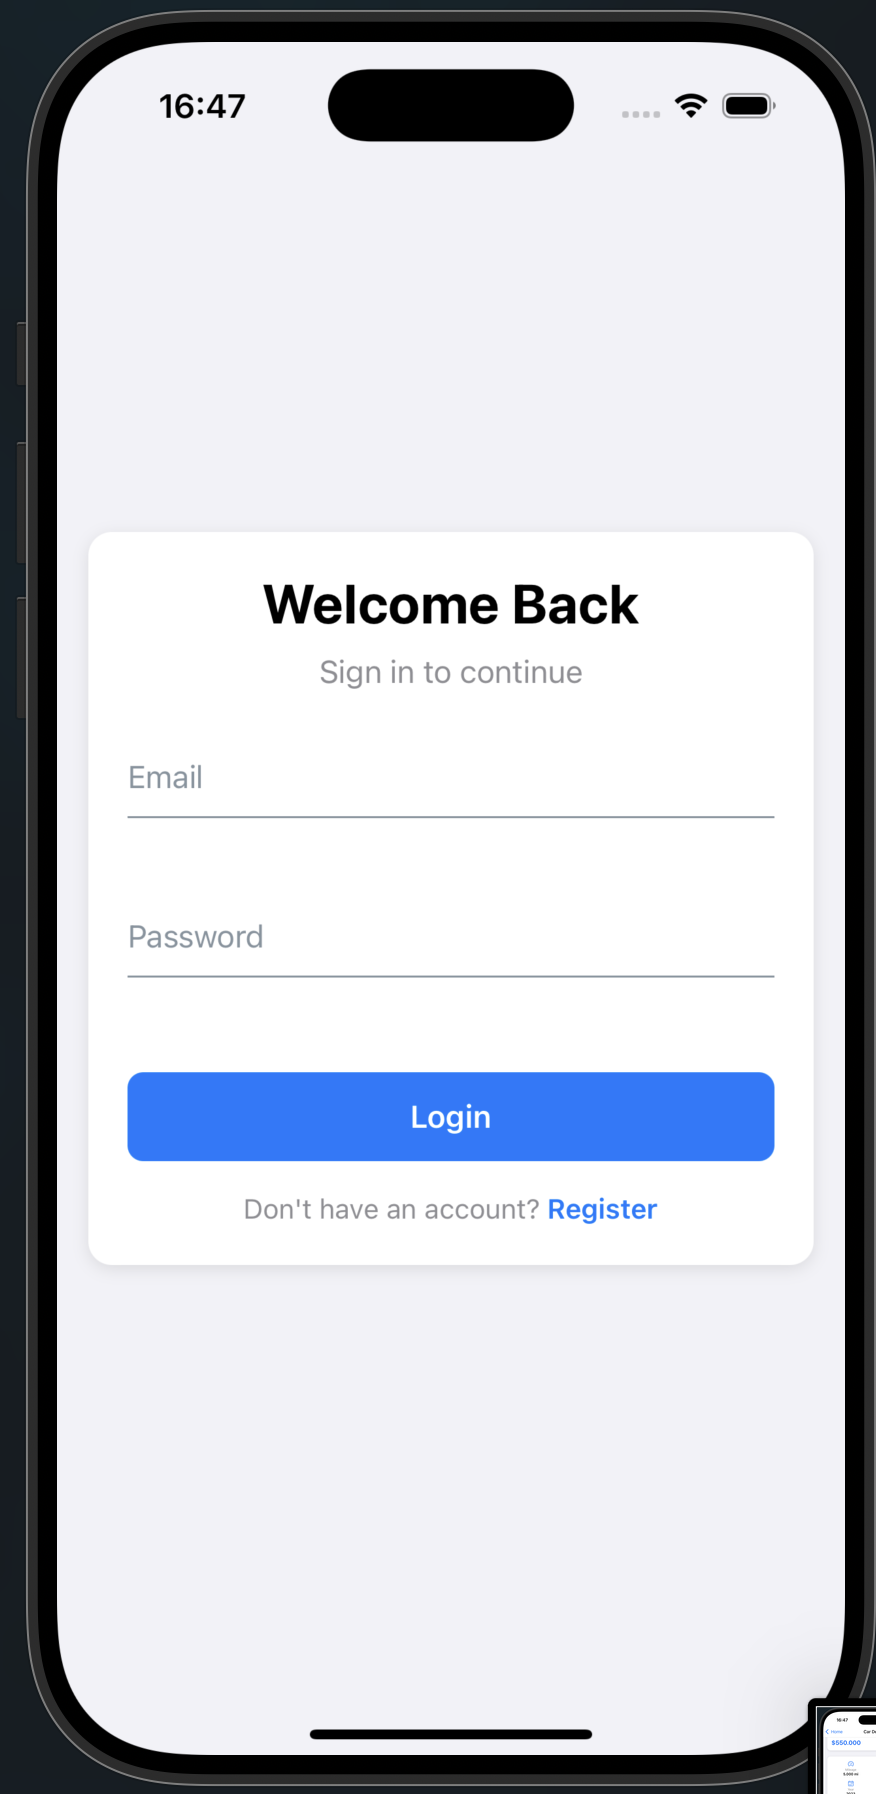
\includegraphics[width=\textwidth]{images/login page.png}
        \caption{Écran de connexion}
        \label{fig:login}
    \end{subfigure}
    \hfill
    \begin{subfigure}[b]{0.48\textwidth}
        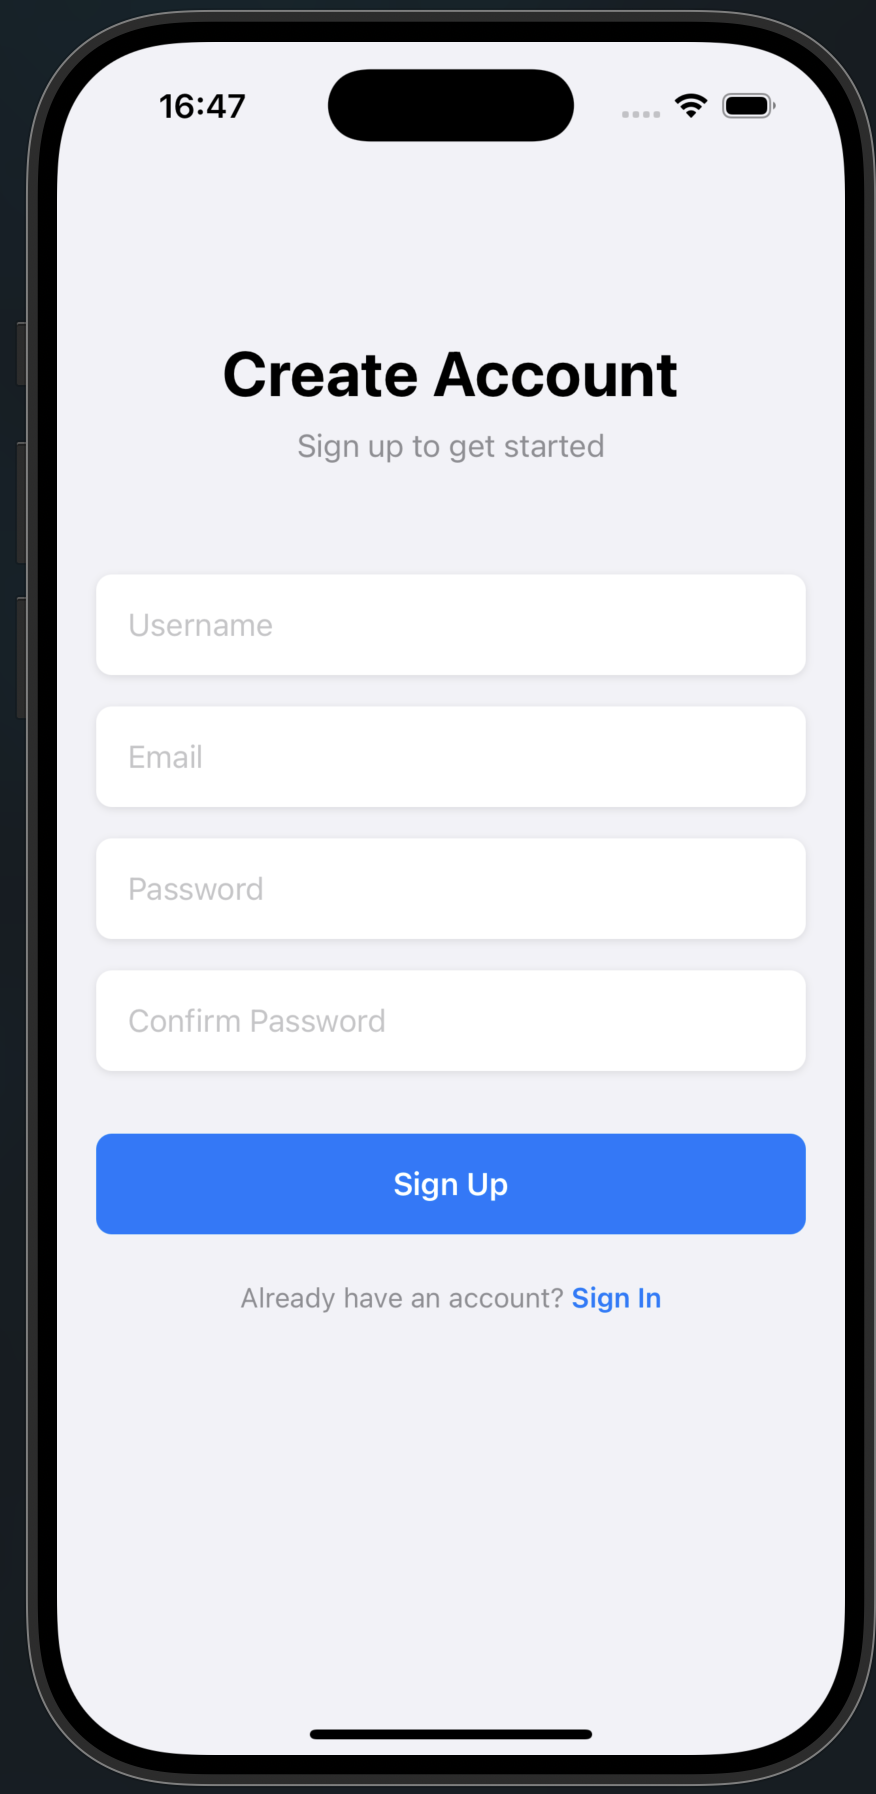
\includegraphics[width=\textwidth]{images/signup page.png}
        \caption{Écran d'inscription}
        \label{fig:register}
    \end{subfigure}
    \caption{Écrans d'authentification de l'application}
    \label{fig:auth-screens}
\end{figure}

L'utilisateur peut accéder à l'application via la page de connexion (Figure \ref{fig:login}) ou créer un nouveau compte via la page d'inscription (Figure \ref{fig:register}). Ces écrans permettent une entrée sécurisée dans le système.

\subsection{Page d'Accueil et Enchères}

\begin{figure}[H]
    \centering
    \begin{subfigure}[b]{0.48\textwidth}
        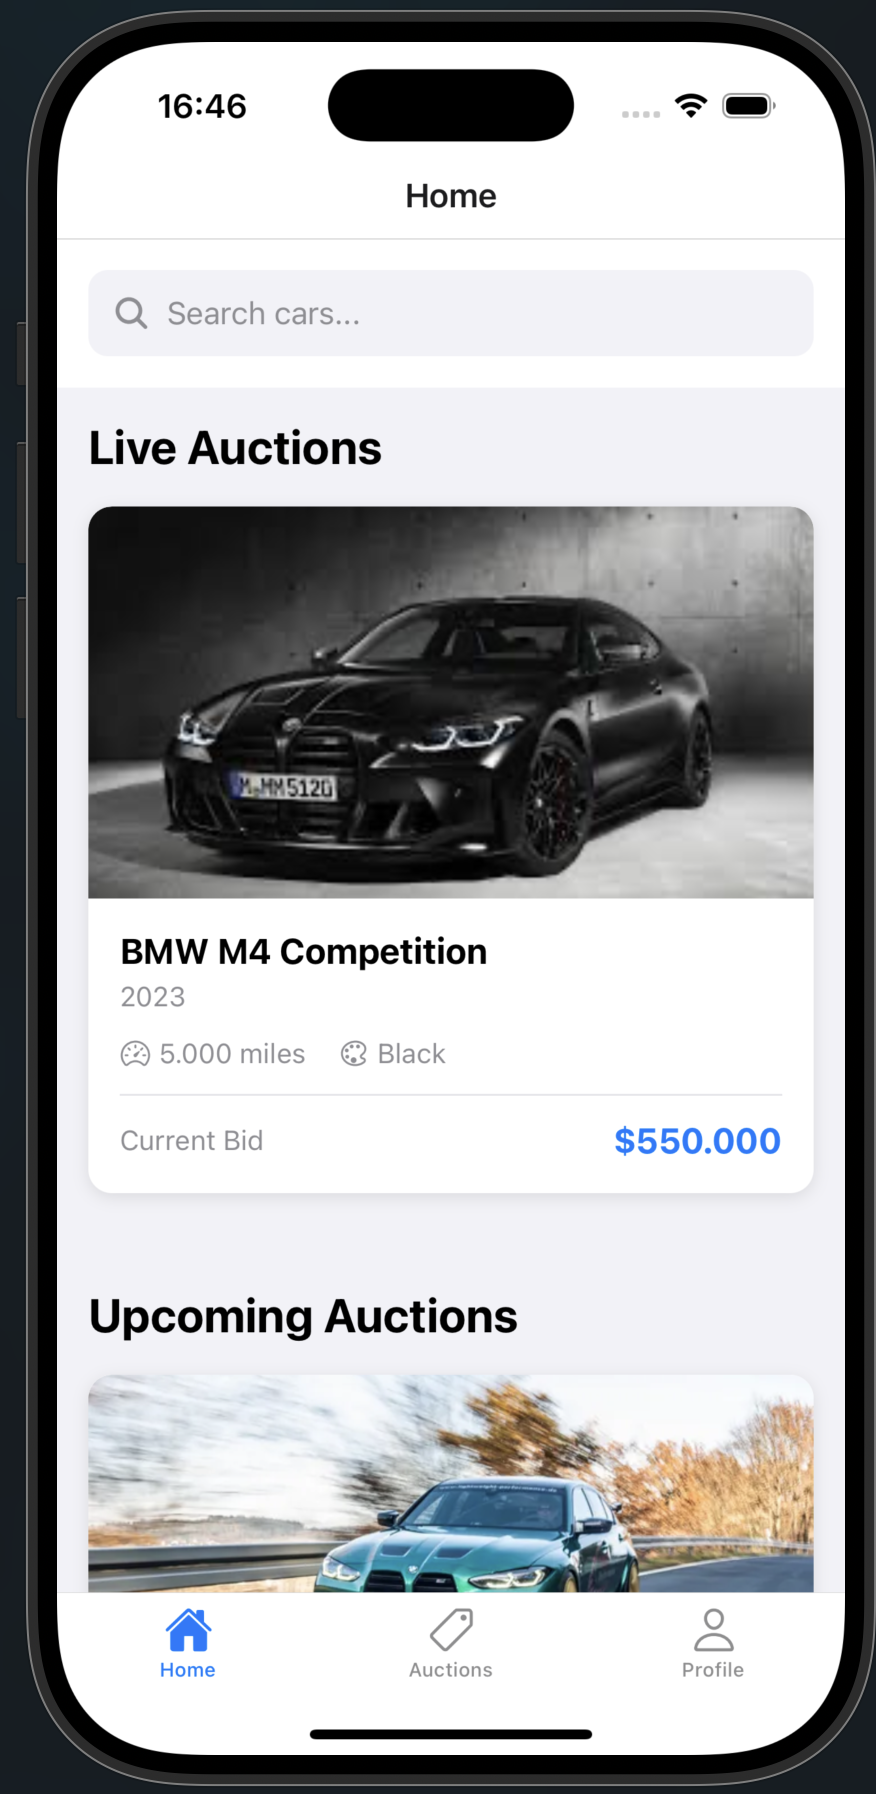
\includegraphics[width=\textwidth]{images/home page with live auctions.png}
        \caption{Enchères en cours}
        \label{fig:home-live}
    \end{subfigure}
    \hfill
    \begin{subfigure}[b]{0.48\textwidth}
        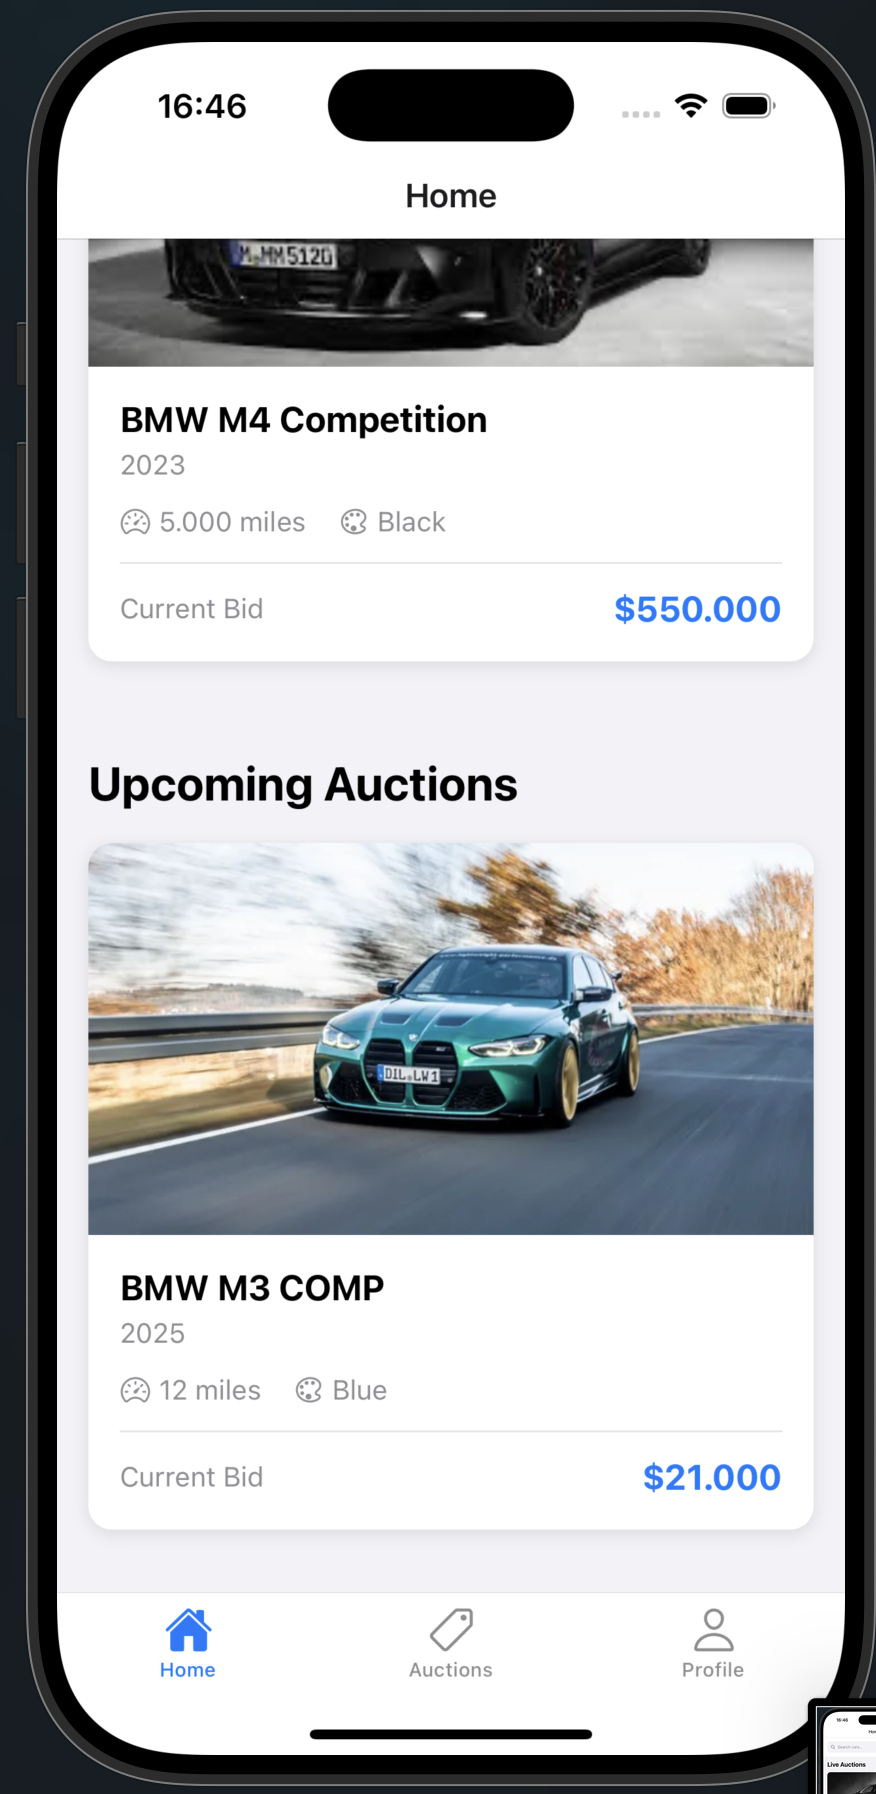
\includegraphics[width=\textwidth]{images/home page with upcoming auctions.png}
        \caption{Enchères à venir}
        \label{fig:home-upcoming}
    \end{subfigure}
    \caption{Pages d'accueil avec différentes vues des enchères}
    \label{fig:home}
\end{figure}

La page d'accueil présente les enchères en cours (Figure \ref{fig:home-live}) et les enchères à venir (Figure \ref{fig:home-upcoming}), permettant aux utilisateurs de parcourir facilement les véhicules disponibles. On y trouve des informations essentielles comme la marque, le modèle, l'année, le kilométrage et le prix actuel de l'enchère.

\subsection{Gestion des Enchères}

\begin{figure}[H]
    \centering
    \begin{subfigure}[b]{0.32\textwidth}
        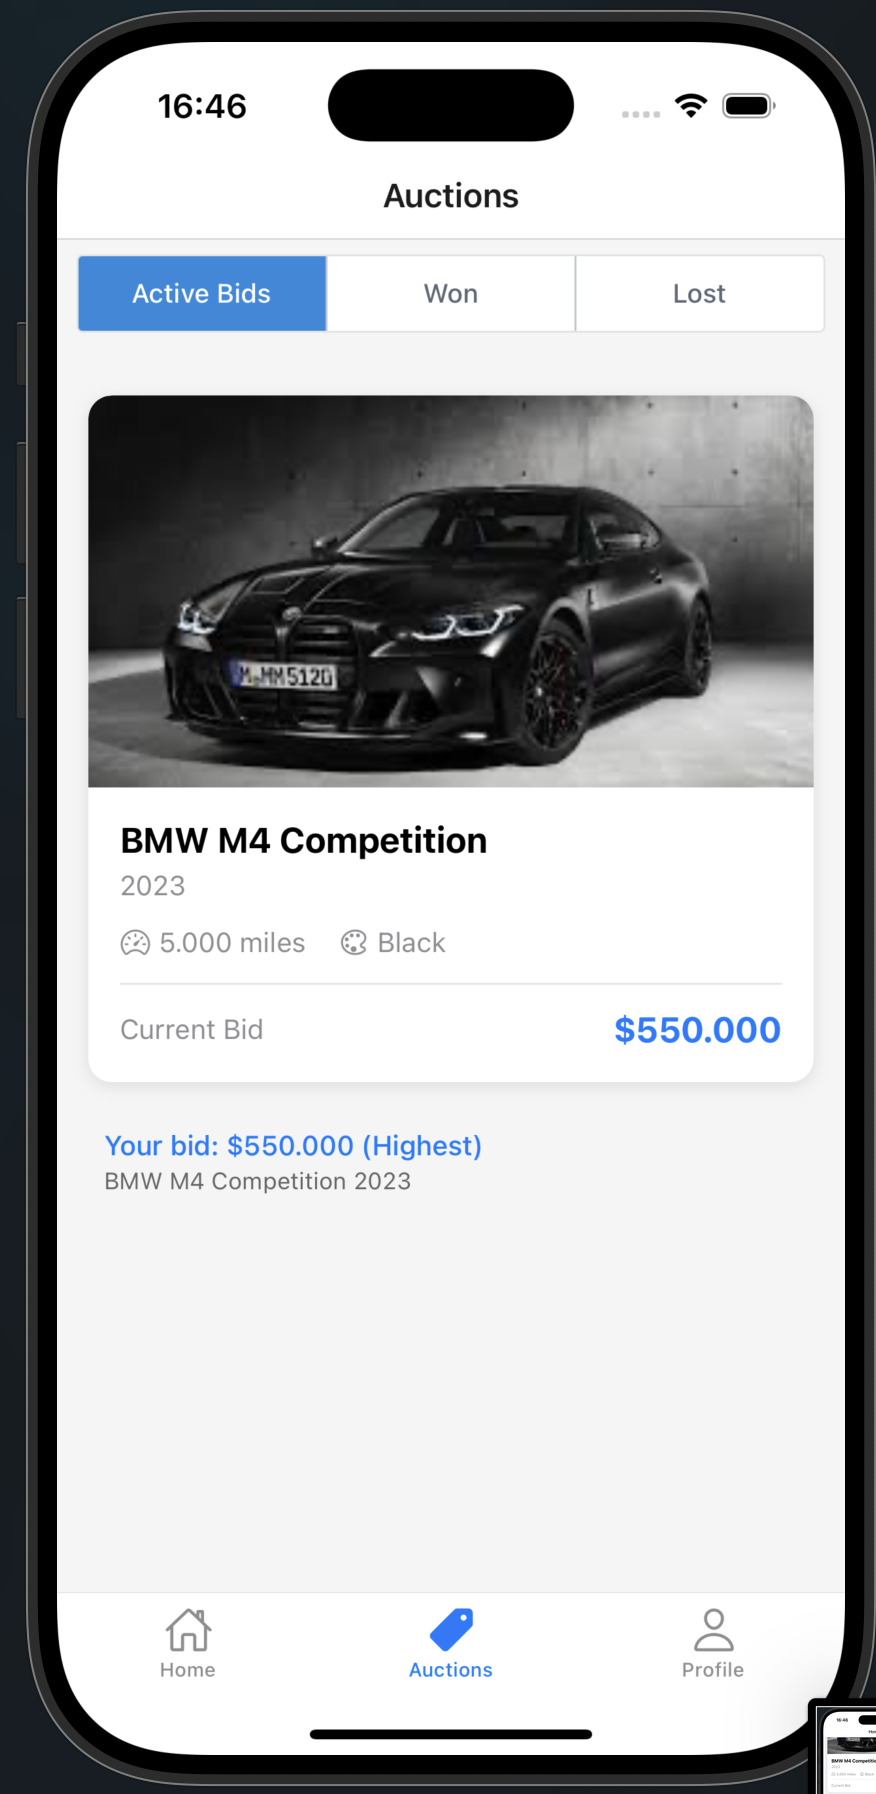
\includegraphics[width=\textwidth]{images/auction page with active bids.png}
        \caption{Enchères actives}
        \label{fig:active-bids}
    \end{subfigure}
    \hfill
    \begin{subfigure}[b]{0.32\textwidth}
        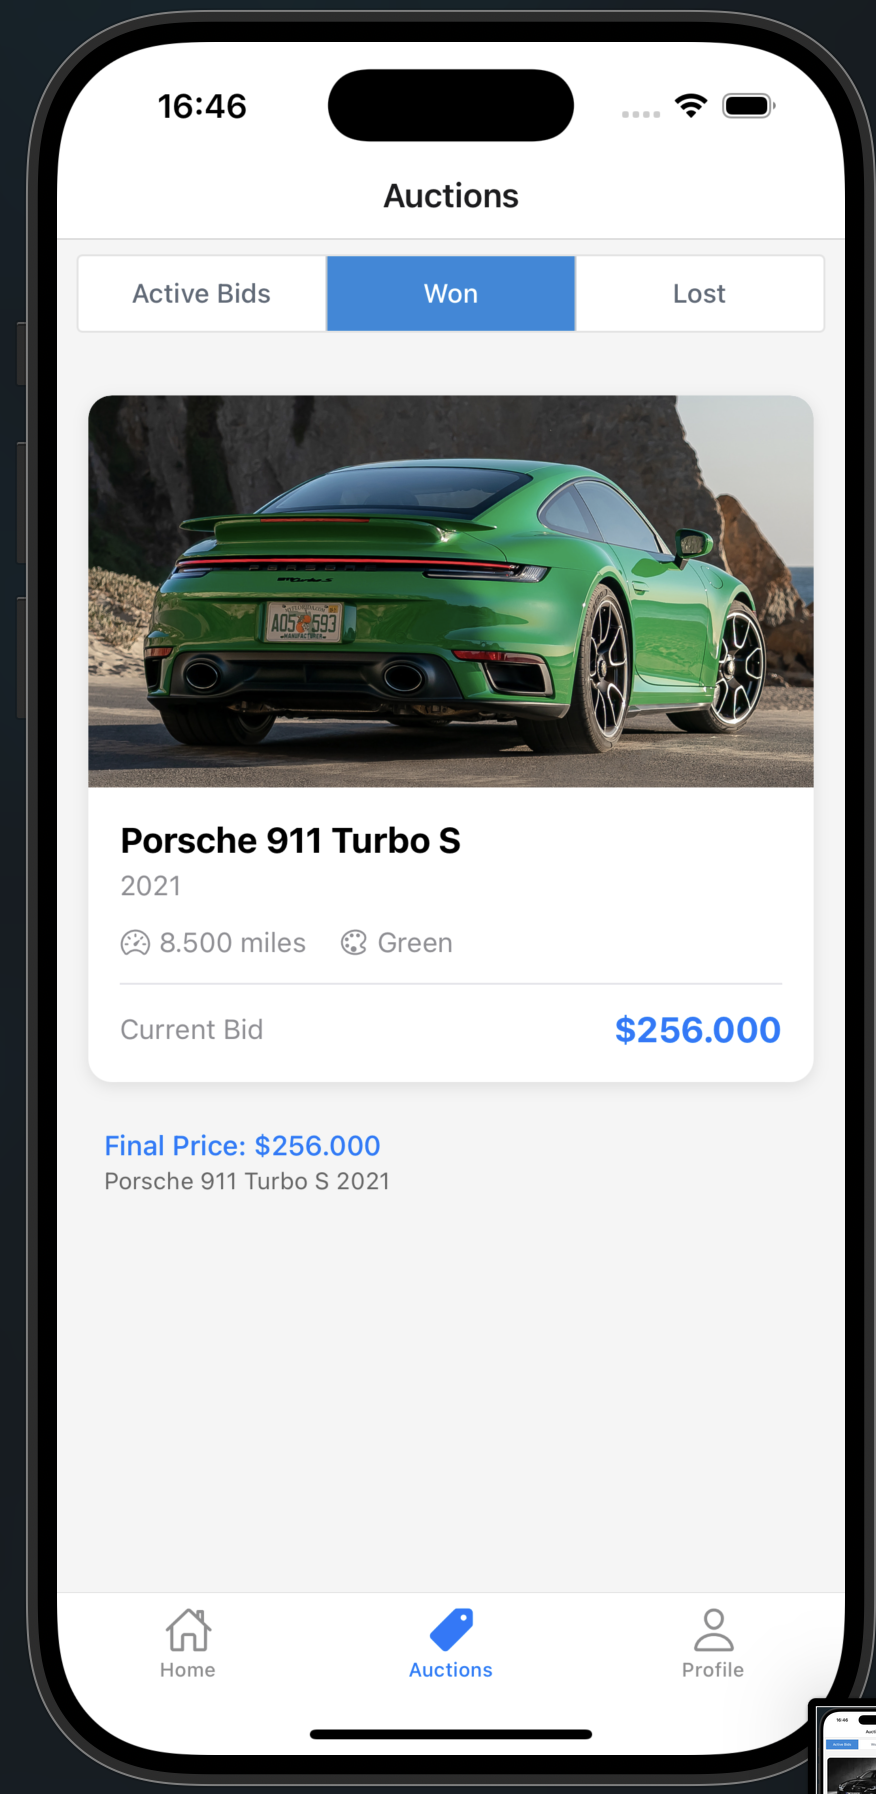
\includegraphics[width=\textwidth]{images/auction page with won bids.png}
        \caption{Enchères gagnées}
        \label{fig:won-auctions}
    \end{subfigure}
    \hfill
    \begin{subfigure}[b]{0.32\textwidth}
        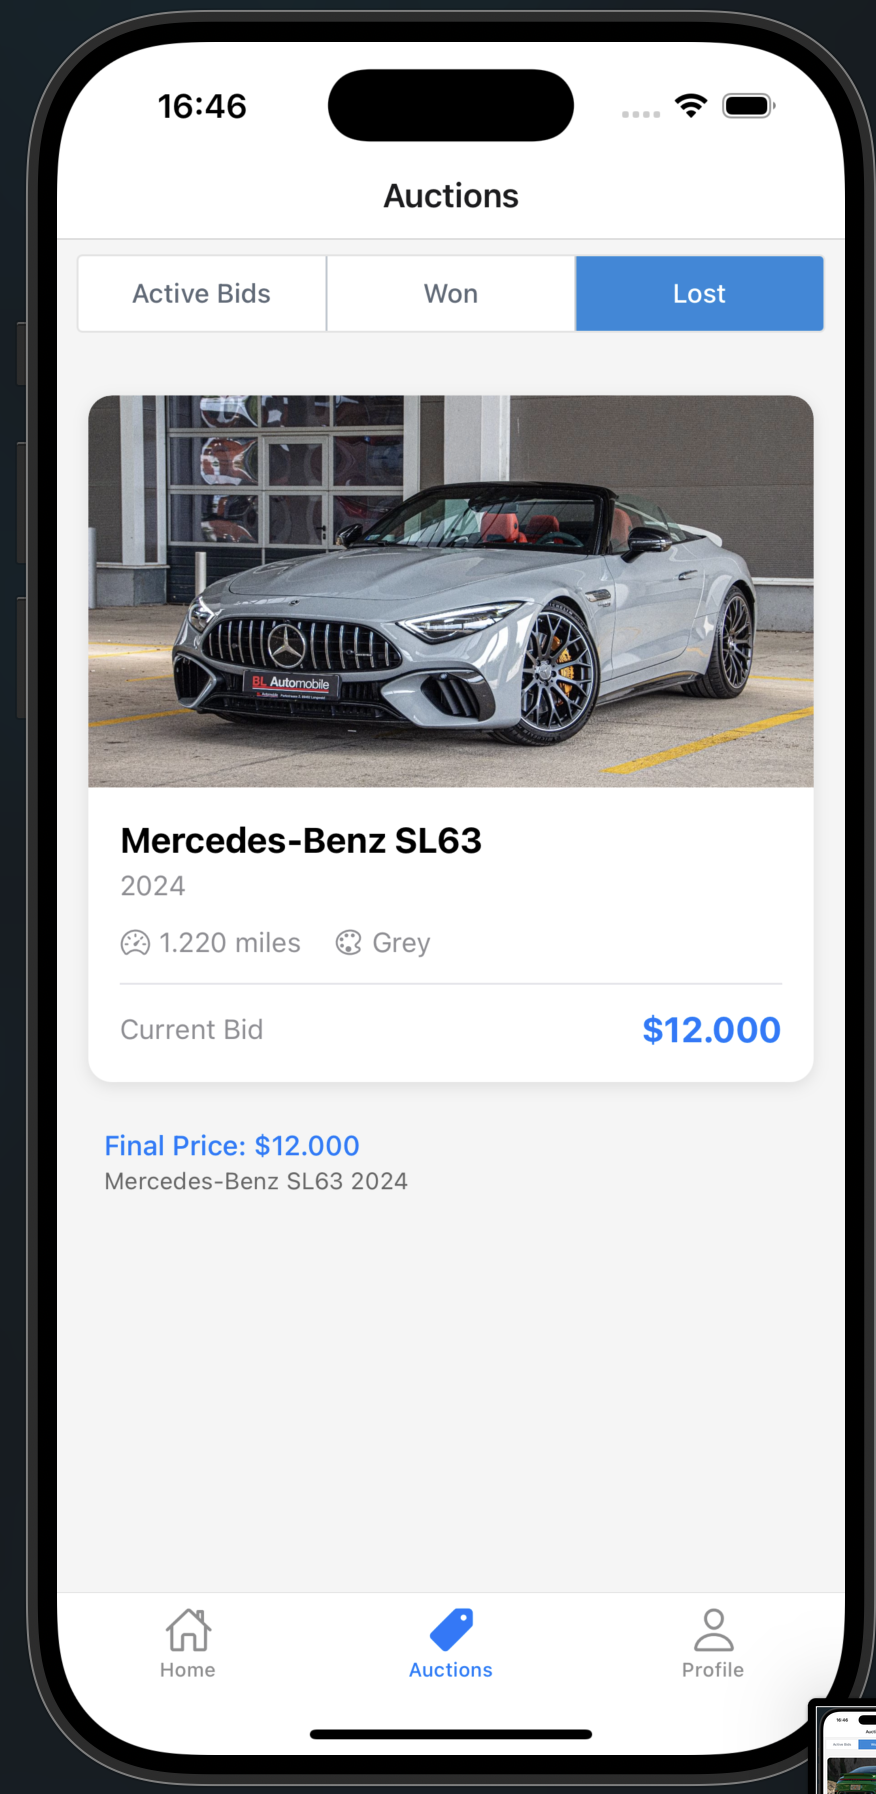
\includegraphics[width=\textwidth]{images/auction page with lost bids.png}
        \caption{Enchères perdues}
        \label{fig:lost-auctions}
    \end{subfigure}
    \caption{Écrans de gestion des enchères}
    \label{fig:auction-management}
\end{figure}

Les utilisateurs peuvent suivre leurs enchères via différents onglets : enchères actives (Figure \ref{fig:active-bids}), enchères gagnées (Figure \ref{fig:won-auctions}) et enchères perdues (Figure \ref{fig:lost-auctions}).

\subsection{Profil Utilisateur}

\begin{figure}[H]
    \centering
    \begin{subfigure}[b]{0.48\textwidth}
        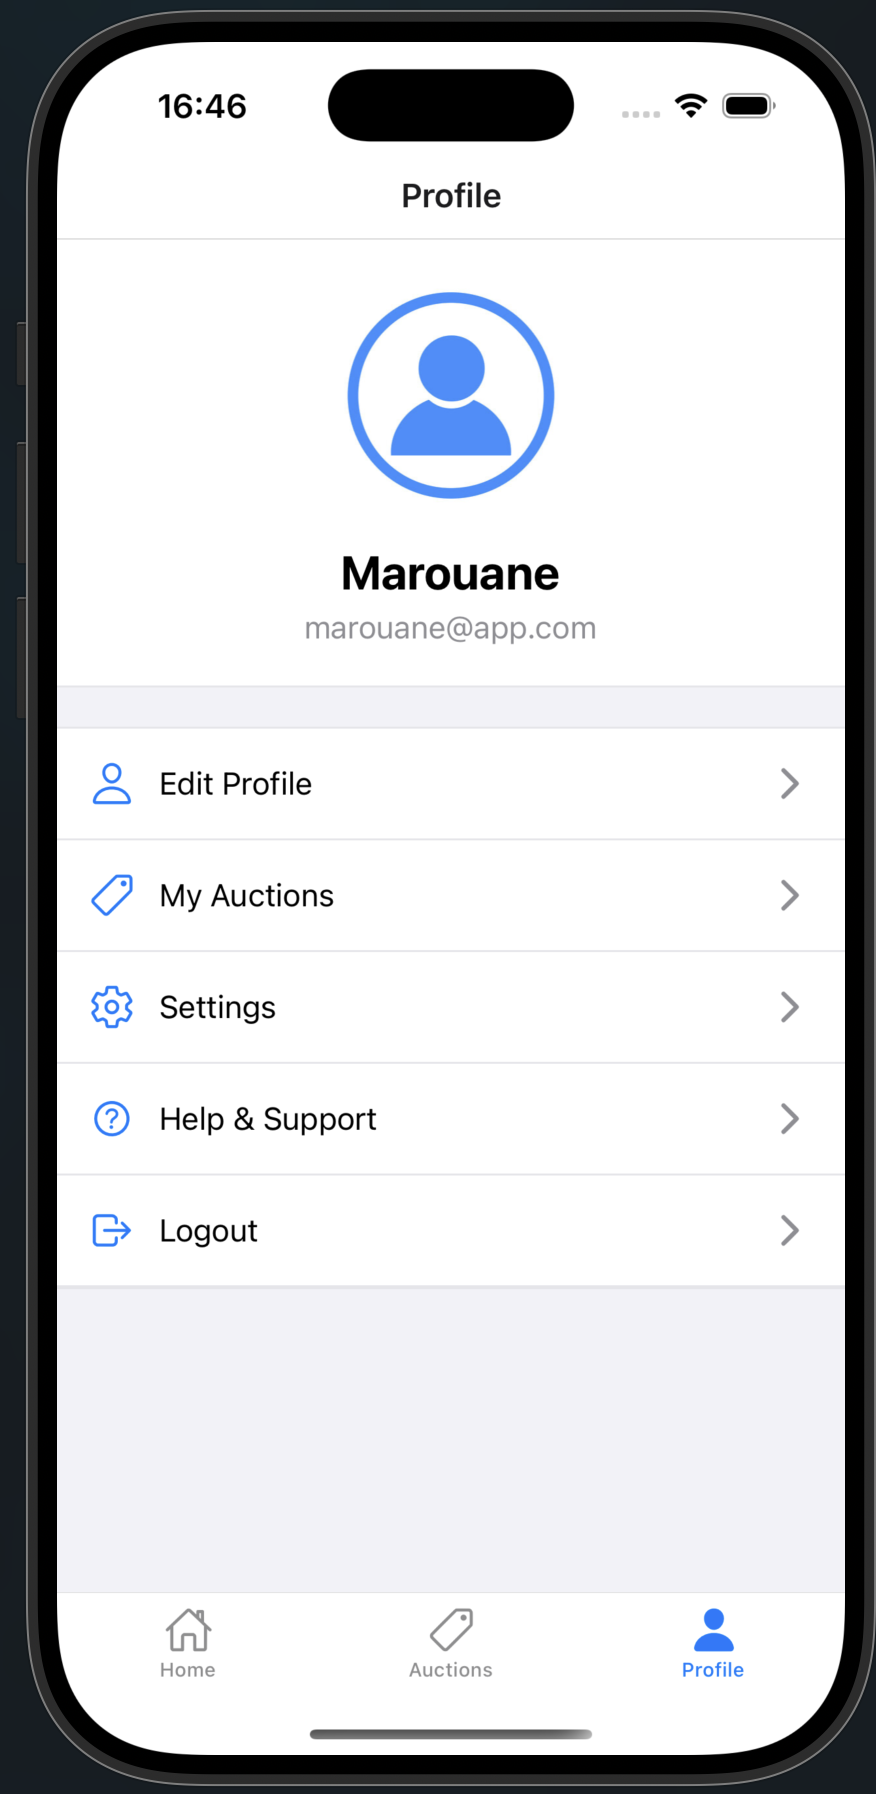
\includegraphics[width=\textwidth]{images/profile screen.png}
        \caption{Écran de profil}
        \label{fig:profile}
    \end{subfigure}
    \hfill
    \begin{subfigure}[b]{0.48\textwidth}
        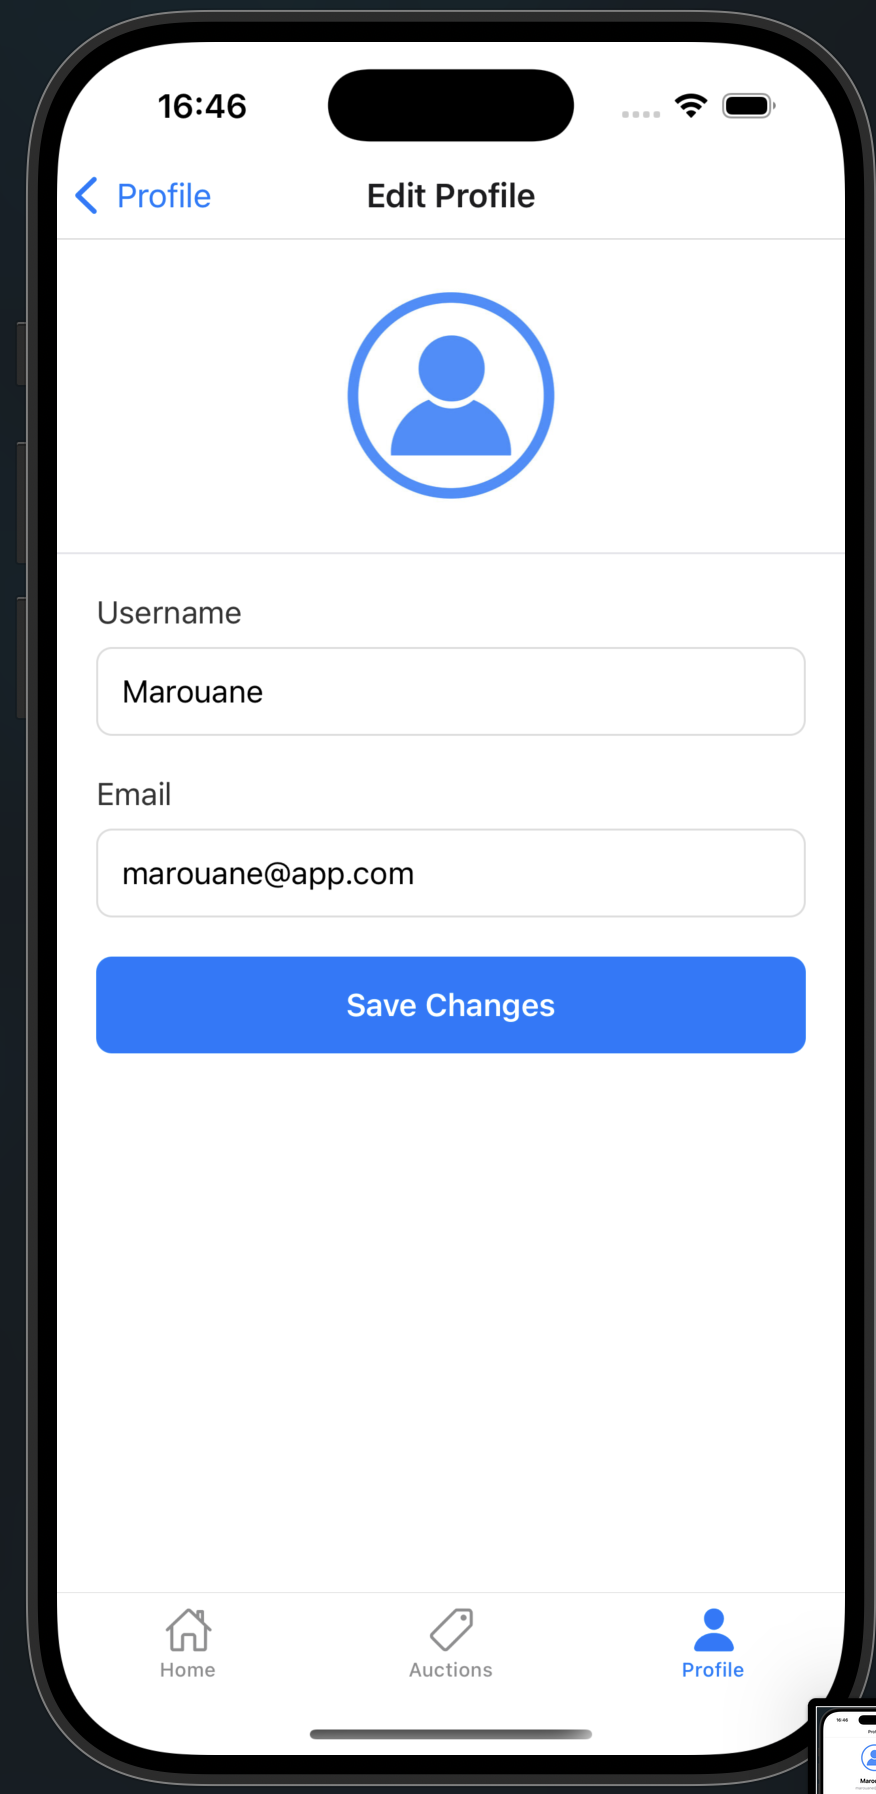
\includegraphics[width=\textwidth]{images/profile edit .png}
        \caption{Modification du profil}
        \label{fig:profile-edit}
    \end{subfigure}
    \caption{Gestion du profil utilisateur}
    \label{fig:profile-management}
\end{figure}

L'écran de profil (Figure \ref{fig:profile}) permet d'accéder aux informations personnelles de l'utilisateur et à l'historique de ses enchères. L'écran de modification du profil (Figure \ref{fig:profile-edit}) permet de mettre à jour les informations personnelles.

\subsection{Détails du Véhicule et Enchère}

\begin{figure}[H]
    \centering
    \begin{subfigure}[b]{0.48\textwidth}
        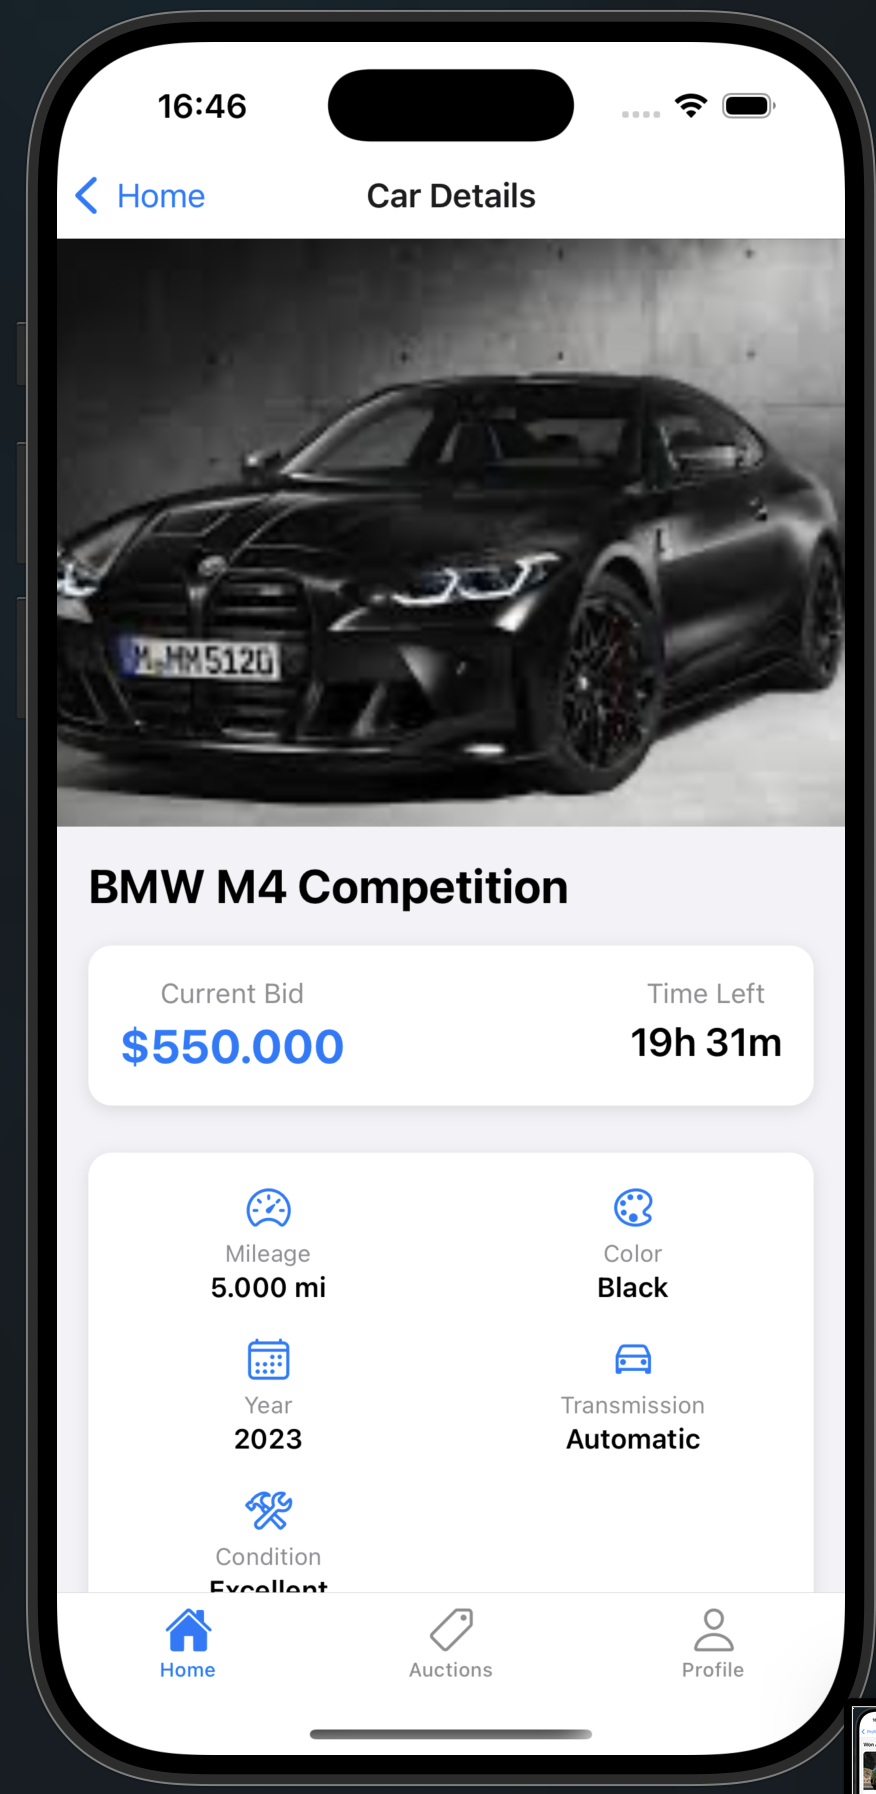
\includegraphics[width=\textwidth]{images/auction details 1 .png}
        \caption{Informations du véhicule}
        \label{fig:car-details1}
    \end{subfigure}
    \hfill
    \begin{subfigure}[b]{0.48\textwidth}
        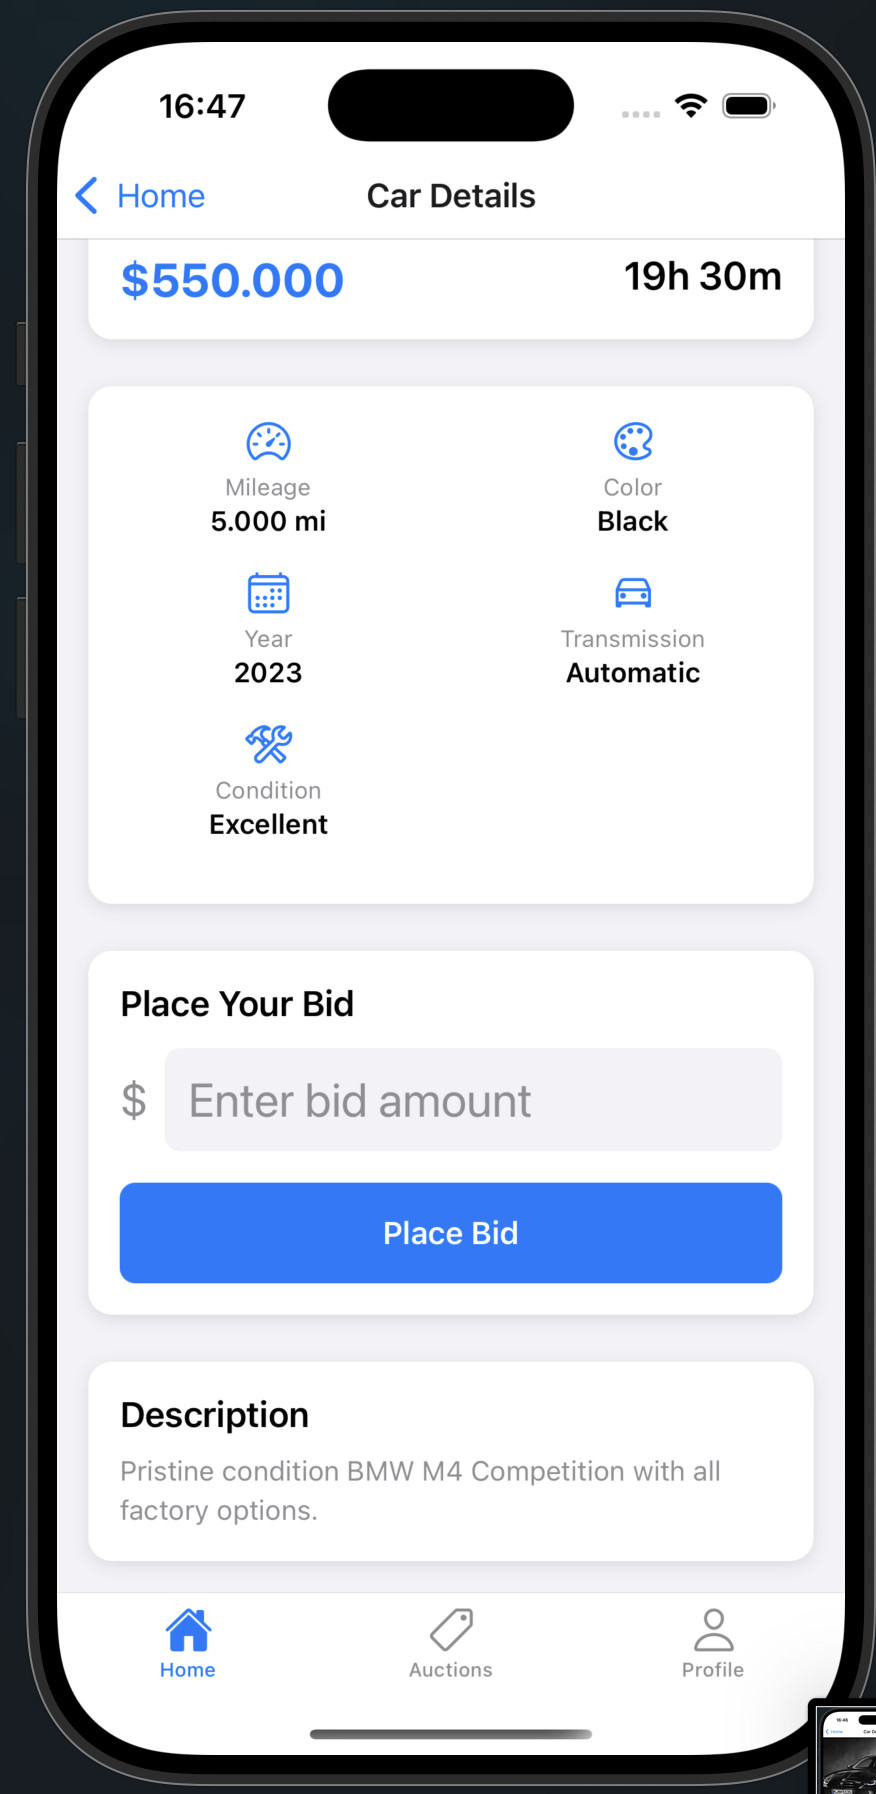
\includegraphics[width=\textwidth]{images/auction details 2.png}
        \caption{Placement d'enchère}
        \label{fig:car-details2}
    \end{subfigure}
    \caption{Détails du véhicule et système d'enchères}
    \label{fig:car-details}
\end{figure}

Les écrans de détails du véhicule (Figures \ref{fig:car-details1} et \ref{fig:car-details2}) présentent toutes les informations pertinentes sur le véhicule et permettent de placer une enchère directement depuis l'application.

\subsection{Historique des Enchères}

\begin{figure}[H]
    \centering
    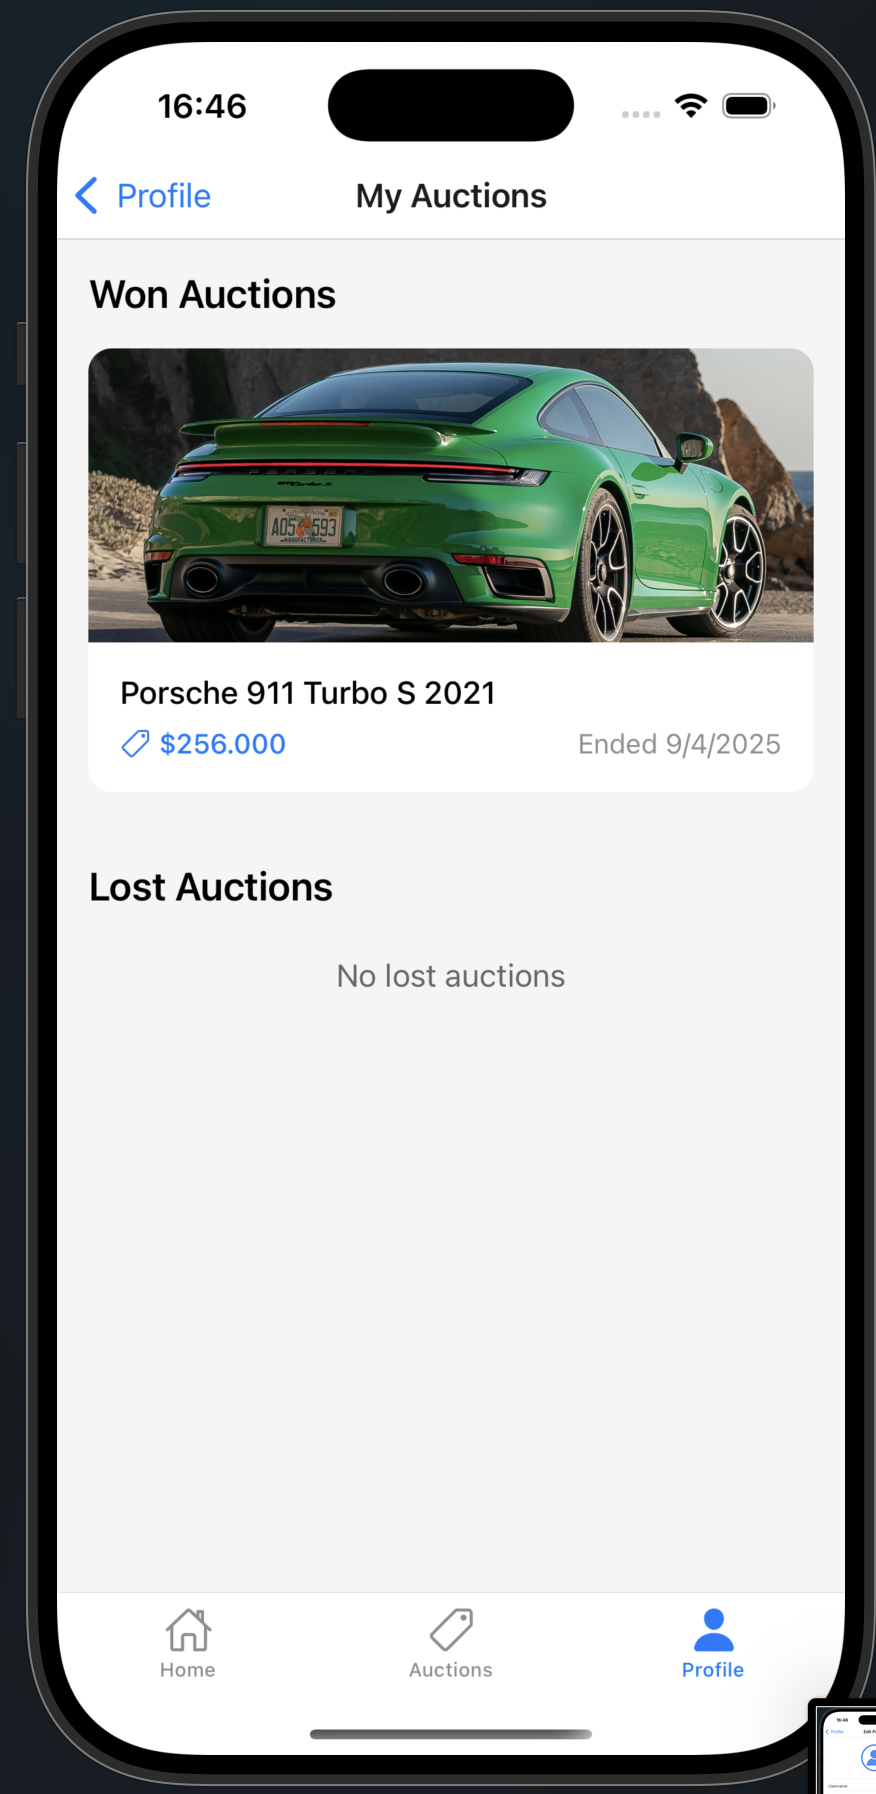
\includegraphics[width=0.6\textwidth]{images/auctions history.png}
    \caption{Historique des enchères de l'utilisateur}
    \label{fig:auction-history}
\end{figure}

L'écran d'historique des enchères (Figure \ref{fig:auction-history}) permet à l'utilisateur de consulter l'ensemble de ses activités d'enchères passées, incluant les véhicules sur lesquels il a enchéri, les montants proposés et les résultats obtenus.

\section{Fonctionnalités Principales}

\begin{itemize}
    \item \textbf{Inscription et connexion} : Création de compte et authentification sécurisée
    \item \textbf{Navigation des enchères} : Parcourir les enchères en cours et à venir
    \item \textbf{Participation aux enchères} : Placer des enchères sur les véhicules désirés
    \item \textbf{Suivi des enchères} : Consulter l'état de vos enchères actives, gagnées et perdues
    \item \textbf{Gestion du profil} : Mettre à jour vos informations personnelles
    \item \textbf{Notifications} : Recevoir des alertes en temps réel sur les enchères suivies
\end{itemize}

\section{Conseils d'Utilisation}

\begin{itemize}
    \item Configurez les notifications pour être informé des changements d'enchères
    \item Vérifiez régulièrement l'onglet "Enchères actives" pour suivre vos enchères en cours
    \item Complétez intégralement votre profil pour faciliter les transactions
    \item Consultez les détails complets du véhicule avant de placer une enchère
    \item Définissez un budget maximum pour chaque enchère pour éviter les dépassements
\end{itemize} 
\chapter{Analyse de l'Existant}

\section{Solutions d'Enchères Existantes}
\subsection{Solutions Traditionnelles}
Les solutions traditionnelles d'enchères automobiles présentent plusieurs caractéristiques :
\begin{itemize}
    \item Enchères physiques nécessitant une présence sur place
    \item Documentation papier et processus manuel
    \item Limitation géographique des participants
    \item Délais importants dans le traitement des enchères
\end{itemize}

\subsection{Solutions Numériques Actuelles}
Plusieurs plateformes numériques existent sur le marché :
\begin{itemize}
    \item Plateformes web uniquement, sans application mobile native
    \item Applications avec fonctionnalités limitées
    \item Systèmes sans mise à jour en temps réel
    \item Interfaces utilisateur complexes
\end{itemize}

\section{Limitations des Solutions Existantes}
\subsection{Problèmes Techniques}
\begin{itemize}
    \item Absence de notifications en temps réel
    \item Manque d'intégration mobile native
    \item Gestion manuelle des statuts d'enchères
    \item Problèmes de performance avec les mises à jour
\end{itemize}

\subsection{Problèmes Fonctionnels}
\begin{itemize}
    \item Interface administrateur limitée
    \item Absence de suivi des enchères perdues
    \item Processus d'enchère non optimisé
    \item Manque de transparence dans les résultats
\end{itemize}

\section{Opportunités d'Amélioration}
\subsection{Aspects Techniques}
\begin{itemize}
    \item Implémentation de Socket.IO pour les mises à jour en temps réel
    \item Développement d'une application mobile native avec React Native
    \item Automatisation de la gestion des statuts d'enchères
    \item Optimisation des performances serveur avec Node.js
\end{itemize}

\subsection{Aspects Fonctionnels}
\begin{itemize}
    \item Interface utilisateur intuitive et moderne
    \item Système complet de notifications
    \item Tableau de bord administratif avancé
    \item Historique détaillé des enchères
\end{itemize}

\section{Analyse des Risques}
\begin{itemize}
    \item Gestion des conflits de ports (3000, 5001, 8081)
    \item Synchronisation des données en temps réel
    \item Sécurité des transactions
    \item Performance sous charge importante
\end{itemize} 
\chapter{Analyse des Besoins}

\section{Méthodologie d'Analyse}

L'analyse des besoins constitue une étape fondamentale dans le développement de notre système d'enchères automobiles. Cette analyse a été menée selon une approche structurée visant à identifier avec précision les exigences fonctionnelles et non fonctionnelles du système.

\subsection{Collecte des Besoins}

La collecte des besoins a été réalisée à travers plusieurs méthodes complémentaires:

\begin{itemize}
    \item \textbf{Entretiens avec les parties prenantes}: Sessions de discussion avec des acheteurs et vendeurs potentiels, des experts du marché automobile, et des professionnels du développement d'applications
    \item \textbf{Analyse concurrentielle}: Étude approfondie des plateformes d'enchères existantes pour identifier les meilleures pratiques et les opportunités d'innovation
    \item \textbf{Ateliers de brainstorming}: Sessions collaboratives pour générer des idées de fonctionnalités et identifier les priorités
    \item \textbf{Questionnaires}: Sondages ciblés pour recueillir les attentes des utilisateurs potentiels
    \item \textbf{Analyse des tendances du marché}: Étude des évolutions récentes dans le domaine des enchères en ligne et du commerce électronique automobile
\end{itemize}

\subsection{Priorisation des Besoins}

Les besoins identifiés ont été priorisés selon la méthode MoSCoW:

\begin{description}
    \item[Must Have] Fonctionnalités essentielles sans lesquelles le système ne peut pas fonctionner correctement
    \item[Should Have] Fonctionnalités importantes mais non critiques pour le lancement initial
    \item[Could Have] Fonctionnalités souhaitables qui apportent une valeur ajoutée mais peuvent être reportées
    \item[Won't Have] Fonctionnalités intéressantes mais explicitement exclues de la version actuelle
\end{description}

Cette priorisation a permis de définir clairement le périmètre du projet et d'établir une feuille de route pour les développements futurs.

\section{Exigences Fonctionnelles}

Les exigences fonctionnelles définissent les comportements spécifiques et les fonctionnalités que le système doit offrir.

\subsection{Gestion des Utilisateurs}

\begin{enumerate}
    \item \textbf{Inscription des utilisateurs (Must Have)}
    \begin{itemize}
        \item Le système doit permettre la création de nouveaux comptes utilisateurs
        \item Les informations minimales requises incluent: nom d'utilisateur, email, mot de passe
        \item Le système doit vérifier l'unicité des emails et noms d'utilisateur
        \item Une confirmation par email doit être envoyée lors de l'inscription
    \end{itemize}
    
    \item \textbf{Authentification (Must Have)}
    \begin{itemize}
        \item Les utilisateurs doivent pouvoir se connecter avec leur email et mot de passe
        \item Le système doit offrir une fonction de récupération de mot de passe
        \item L'authentification doit être sécurisée par des tokens JWT
        \item Les sessions doivent expirer après une période d'inactivité
    \end{itemize}
    
    \item \textbf{Gestion de profil (Should Have)}
    \begin{itemize}
        \item Les utilisateurs doivent pouvoir modifier leurs informations personnelles
        \item Le téléchargement d'une photo de profil doit être possible
        \item L'historique des activités (enchères placées, remportées) doit être consultable
        \item Les préférences de notification doivent être configurables
    \end{itemize}
    
    \item \textbf{Rôles et permissions (Must Have)}
    \begin{itemize}
        \item Le système doit distinguer au moins deux types d'utilisateurs: standard et administrateur
        \item Les administrateurs doivent avoir accès à des fonctionnalités de gestion avancées
        \item Les permissions doivent être vérifiées pour toutes les actions sensibles
    \end{itemize}
\end{enumerate}

\subsection{Gestion des Véhicules}

\begin{enumerate}
    \item \textbf{Ajout de véhicules (Must Have)}
    \begin{itemize}
        \item Les administrateurs doivent pouvoir ajouter de nouveaux véhicules au système
        \item Les informations à saisir incluent: marque, modèle, année, kilométrage, couleur, etc.
        \item Le téléchargement de multiples images doit être supporté
        \item Une description détaillée du véhicule doit être possible
    \end{itemize}
    
    \item \textbf{Modification des véhicules (Should Have)}
    \begin{itemize}
        \item Les informations des véhicules doivent être modifiables tant qu'ils ne sont pas en enchère
        \item L'ajout, la suppression et la réorganisation des images doivent être possibles
        \item Un historique des modifications doit être conservé
    \end{itemize}
    
    \item \textbf{Suppression des véhicules (Should Have)}
    \begin{itemize}
        \item Les véhicules sans enchère active doivent pouvoir être supprimés
        \item Une confirmation doit être demandée avant suppression
        \item La suppression doit être logique plutôt que physique pour préserver l'historique
    \end{itemize}
    
    \item \textbf{Visualisation des véhicules (Must Have)}
    \begin{itemize}
        \item Les utilisateurs doivent pouvoir consulter les détails complets des véhicules
        \item Une galerie d'images avec fonction de zoom doit être disponible
        \item Les caractéristiques techniques doivent être présentées de manière structurée
        \item L'historique d'entretien, si disponible, doit être accessible
    \end{itemize}
\end{enumerate}

\subsection{Gestion des Enchères}

\begin{enumerate}
    \item \textbf{Création d'enchères (Must Have)}
    \begin{itemize}
        \item Les administrateurs doivent pouvoir créer de nouvelles enchères
        \item Chaque enchère doit être associée à un véhicule spécifique
        \item Les paramètres à définir incluent: prix de départ, incrément minimal, dates de début et fin
        \item Des règles spécifiques (extension automatique, prix de réserve) doivent être configurables
    \end{itemize}
    
    \item \textbf{Participation aux enchères (Must Have)}
    \begin{itemize}
        \item Les utilisateurs authentifiés doivent pouvoir placer des enchères
        \item Le montant proposé doit être supérieur au prix actuel plus l'incrément minimal
        \item L'utilisateur doit recevoir une confirmation immédiate de son enchère
        \item L'historique des enchères doit être visible pour tous les participants
    \end{itemize}
    
    \item \textbf{Suivi des enchères (Must Have)}
    \begin{itemize}
        \item Les utilisateurs doivent pouvoir suivre l'évolution des enchères en temps réel
        \item Un compte à rebours doit indiquer le temps restant
        \item Les notifications doivent être envoyées en cas de surenchère
        \item Les enchères terminées doivent être clairement identifiées avec leur résultat
    \end{itemize}
    
    \item \textbf{Finalisation des enchères (Should Have)}
    \begin{itemize}
        \item Les enchères doivent se terminer automatiquement à la date et heure définies
        \item Le gagnant doit être déterminé et notifié automatiquement
        \item Un récapitulatif doit être généré pour le vendeur et l'acheteur
        \item Les enchères sans offre valide doivent être marquées comme non attribuées
    \end{itemize}
\end{enumerate}

\subsection{Notifications et Communication}

\begin{enumerate}
    \item \textbf{Notifications en temps réel (Must Have)}
    \begin{itemize}
        \item Les utilisateurs doivent recevoir des notifications push pour les événements importants
        \item Les notifications doivent inclure: surenchères, fin imminente, enchère remportée/perdue
        \item Les notifications doivent être personnalisables selon les préférences utilisateur
    \end{itemize}
    
    \item \textbf{Alertes par email (Should Have)}
    \begin{itemize}
        \item Des emails doivent être envoyés pour les événements majeurs
        \item Les contenus des emails doivent être personnalisés et professionnels
        \item Une option de désabonnement doit être disponible
    \end{itemize}
    
    \item \textbf{Centre de notifications (Could Have)}
    \begin{itemize}
        \item Un centre de notifications dans l'application doit centraliser tous les messages
        \item Les notifications doivent pouvoir être marquées comme lues/non lues
        \item Un historique des notifications doit être conservé
    \end{itemize}
\end{enumerate}

\subsection{Recherche et Filtrage}

\begin{enumerate}
    \item \textbf{Recherche de véhicules (Must Have)}
    \begin{itemize}
        \item Les utilisateurs doivent pouvoir rechercher des véhicules par mots-clés
        \item La recherche doit porter sur les marques, modèles, descriptions, etc.
        \item Les résultats doivent être pertinents et classés par ordre de pertinence
    \end{itemize}
    
    \item \textbf{Filtrage avancé (Should Have)}
    \begin{itemize}
        \item Des filtres multiples doivent être disponibles: marque, modèle, année, prix, etc.
        \item Les filtres doivent être combinables pour affiner les résultats
        \item Les valeurs de filtrage doivent être présentées de manière intuitive (sliders, listes déroulantes)
    \end{itemize}
    
    \item \textbf{Tri des résultats (Should Have)}
    \begin{itemize}
        \item Les résultats doivent pouvoir être triés selon différents critères
        \item Les options de tri incluent: prix (croissant/décroissant), popularité, fin prochaine
        \item Le tri sélectionné doit être mémorisé pendant la session
    \end{itemize}
\end{enumerate}

\subsection{Administration}

\begin{enumerate}
    \item \textbf{Tableau de bord administrateur (Must Have)}
    \begin{itemize}
        \item Un tableau de bord doit présenter les statistiques clés du système
        \item Des graphiques d'activité doivent visualiser les tendances
        \item Des alertes doivent signaler les situations nécessitant attention
    \end{itemize}
    
    \item \textbf{Gestion des utilisateurs (Should Have)}
    \begin{itemize}
        \item Les administrateurs doivent pouvoir consulter, modifier et suspendre des comptes
        \item Des filtres doivent permettre de rechercher rapidement des utilisateurs
        \item L'historique d'activité des utilisateurs doit être accessible
    \end{itemize}
    
    \item \textbf{Modération des enchères (Should Have)}
    \begin{itemize}
        \item Les administrateurs doivent pouvoir intervenir sur les enchères en cours
        \item Les options incluent: pause, annulation, extension, modification du prix
        \item Toute intervention doit être journalisée avec justification
    \end{itemize}
    
    \item \textbf{Rapports et analyses (Could Have)}
    \begin{itemize}
        \item Des rapports détaillés doivent être générables sur différentes métriques
        \item Les rapports peuvent concerner: ventes, utilisateurs, performances, etc.
        \item L'exportation des données doit être possible en différents formats
    \end{itemize}
\end{enumerate}

\section{Exigences Non Fonctionnelles}

Les exigences non fonctionnelles définissent les critères de qualité et les contraintes auxquelles le système doit se conformer.

\subsection{Performance}

\begin{enumerate}
    \item \textbf{Temps de réponse (Must Have)}
    \begin{itemize}
        \item Le temps de chargement initial de l'application ne doit pas excéder 3 secondes
        \item Les interactions utilisateur doivent recevoir une réponse en moins de 1 seconde
        \item La mise à jour des enchères en temps réel doit s'effectuer en moins de 500 ms
    \end{itemize}
    
    \item \textbf{Capacité de charge (Should Have)}
    \begin{itemize}
        \item Le système doit supporter simultanément au moins 1000 utilisateurs actifs
        \item Jusqu'à 100 enchères simultanées doivent être gérables sans dégradation
        \item Le système doit pouvoir traiter au moins 50 enchères par minute
    \end{itemize}
    
    \item \textbf{Scalabilité (Should Have)}
    \begin{itemize}
        \item L'architecture doit permettre une mise à l'échelle horizontale
        \item Les pics d'activité doivent être absorbables par allocation dynamique de ressources
        \item La performance ne doit pas se dégrader significativement avec l'augmentation du volume de données
    \end{itemize}
\end{enumerate}

\subsection{Sécurité}

\begin{enumerate}
    \item \textbf{Authentification et autorisation (Must Have)}
    \begin{itemize}
        \item Les mots de passe doivent être stockés avec un hachage fort (bcrypt)
        \item L'authentification multi-facteurs doit être disponible
        \item Les sessions doivent expirer automatiquement après 30 minutes d'inactivité
        \item Les autorisations doivent être vérifiées à chaque action sensible
    \end{itemize}
    
    \item \textbf{Protection des données (Must Have)}
    \begin{itemize}
        \item Toutes les communications doivent être chiffrées via HTTPS
        \item Les données sensibles doivent être chiffrées au repos
        \item Les accès aux données doivent être tracés et auditables
        \item La conformité RGPD doit être assurée pour les utilisateurs européens
    \end{itemize}
    
    \item \textbf{Sécurité applicative (Should Have)}
    \begin{itemize}
        \item Protection contre les injections SQL et NoSQL
        \item Défense contre les attaques XSS et CSRF
        \item Limitation du débit des requêtes pour prévenir les attaques DDoS
        \item Validation stricte des entrées utilisateur côté serveur
    \end{itemize}
\end{enumerate}

\subsection{Fiabilité}

\begin{enumerate}
    \item \textbf{Disponibilité (Must Have)}
    \begin{itemize}
        \item Le système doit garantir une disponibilité de 99,9\% (hors maintenance planifiée)
        \item Les temps d'arrêt planifiés doivent être annoncés au moins 24h à l'avance
        \item Un plan de reprise après sinistre doit être en place avec RTO < 4h
    \end{itemize}
    
    \item \textbf{Robustesse (Should Have)}
    \begin{itemize}
        \item Le système doit gérer gracieusement les erreurs côté client et serveur
        \item Les transactions critiques doivent être protégées contre les défaillances
        \item La reconnexion automatique doit être implémentée pour les communications temps réel
    \end{itemize}
    
    \item \textbf{Intégrité des données (Must Have)}
    \begin{itemize}
        \item Les transactions impliquant des enchères doivent être atomiques
        \item Des sauvegardes régulières doivent être effectuées avec RPO < 1h
        \item La cohérence des données doit être vérifiable par des processus automatisés
    \end{itemize}
\end{enumerate}

\subsection{Utilisabilité}

\begin{enumerate}
    \item \textbf{Interface utilisateur (Must Have)}
    \begin{itemize}
        \item L'interface doit être intuitive et nécessiter un minimum de formation
        \item La navigation doit être cohérente à travers toute l'application
        \item Le design doit s'adapter aux différentes tailles d'écran (responsive)
    \end{itemize}
    
    \item \textbf{Accessibilité (Should Have)}
    \begin{itemize}
        \item L'application doit être conforme aux normes WCAG 2.1 niveau AA
        \item Le contraste des couleurs doit être suffisant pour les utilisateurs malvoyants
        \item Des alternatives textuelles doivent être fournies pour tous les éléments visuels
    \end{itemize}
    
    \item \textbf{Internationalisation (Could Have)}
    \begin{itemize}
        \item L'interface doit supporter plusieurs langues
        \item Les formats de date, heure et devise doivent s'adapter aux paramètres régionaux
        \item Le contenu doit être adaptable aux spécificités culturelles
    \end{itemize}
\end{enumerate}

\subsection{Compatibilité}

\begin{enumerate}
    \item \textbf{Compatibilité mobile (Must Have)}
    \begin{itemize}
        \item L'application doit fonctionner sur iOS 12+ et Android 8+
        \item L'interface doit s'adapter aux différentes résolutions d'écran
        \item Les fonctionnalités doivent être cohérentes entre plateformes
    \end{itemize}
    
    \item \textbf{Compatibilité navigateur (Should Have)}
    \begin{itemize}
        \item Une version web progressive doit être compatible avec les navigateurs modernes
        \item Le support minimum inclut: Chrome 70+, Firefox 60+, Safari 12+, Edge 79+
        \item Les fonctionnalités dégradées gracieusement selon les capacités du navigateur
    \end{itemize}
    
    \item \textbf{Intégration API (Could Have)}
    \begin{itemize}
        \item Des API publiques doivent être disponibles pour intégration tierce
        \item Les API doivent être documentées selon les standards OpenAPI
        \item Des environnements de test et de staging doivent être fournis
    \end{itemize}
\end{enumerate}

\section{Contraintes Techniques}

\begin{enumerate}
    \item \textbf{Infrastructure}
    \begin{itemize}
        \item Le système doit être déployable sur des infrastructures cloud (AWS, GCP, Azure)
        \item Les composants doivent être conteneurisés pour faciliter le déploiement
        \item L'architecture doit supporter la réplication géographique
    \end{itemize}
    
    \item \textbf{Développement}
    \begin{itemize}
        \item Le code source doit être versionné avec Git
        \item Le développement doit suivre une approche CI/CD
        \item Des tests automatisés doivent couvrir au moins 80\% du code
    \end{itemize}
    
    \item \textbf{Maintenance}
    \begin{itemize}
        \item La documentation technique doit être maintenue à jour
        \item Le code doit suivre des standards de qualité vérifiables automatiquement
        \item Des logs détaillés doivent être générés pour faciliter le débogage
    \end{itemize}
\end{enumerate}

\section{Scénarios d'Utilisation}

Pour illustrer concrètement les besoins identifiés, plusieurs scénarios d'utilisation ont été définis:

\subsection{Scénario 1: Inscription et Première Enchère}

\begin{quote}
Jean découvre l'application d'enchères automobiles et décide de s'inscrire. Après avoir créé son compte et complété son profil, il parcourt les enchères en cours. Un véhicule attire son attention: une Peugeot 308 de 2018 avec 45,000 km. L'enchère se termine dans 3 heures et le prix actuel est de 12,500€. Jean décide de placer une enchère à 12,700€. Il reçoit une confirmation immédiate et peut voir son nom apparaître comme enchérisseur principal. Une heure plus tard, il reçoit une notification l'informant qu'il a été surenchéri. Il retourne dans l'application et place une nouvelle enchère à 13,100€.
\end{quote}

Ce scénario illustre le processus d'inscription, la navigation dans les enchères, le placement d'enchères et le système de notification.

\subsection{Scénario 2: Gestion d'une Enchère par un Administrateur}

\begin{quote}
Marie, administratrice de la plateforme, doit ajouter un nouveau véhicule: une Audi A3 de 2020. Elle se connecte au panneau d'administration, crée une nouvelle fiche véhicule avec toutes les informations techniques, télécharge 8 photos de la voiture, et rédige une description détaillée. Elle configure ensuite une nouvelle enchère avec un prix de départ de 18,000€, un incrément minimal de 200€, et programme son démarrage pour le lendemain à 10h00, avec une durée de 3 jours. Deux jours plus tard, elle constate que l'enchère génère beaucoup d'intérêt et décide de vérifier les participants. Elle peut voir que 15 personnes ont placé un total de 28 enchères, et que le prix actuel est de 22,600€.
\end{quote}

Ce scénario illustre les fonctionnalités d'administration, la création de véhicules et d'enchères, ainsi que le suivi des enchères en cours.

\subsection{Scénario 3: Finalisation d'une Enchère Réussie}

\begin{quote}
L'enchère pour la Toyota Yaris 2019 vient de se terminer. Thomas, qui avait placé la dernière enchère à 14,800€, reçoit une notification l'informant qu'il a remporté l'enchère. Simultanément, l'administrateur reçoit une alerte de fin d'enchère réussie. Le système met automatiquement à jour le statut de l'enchère à "Terminée" et marque Thomas comme gagnant. Thomas reçoit un email récapitulatif avec les détails du véhicule et les prochaines étapes pour finaliser l'achat. Il peut également consulter ces informations dans la section "Mes enchères remportées" de son profil.
\end{quote}

Ce scénario illustre le processus de finalisation d'une enchère, les notifications automatiques et la gestion post-enchère.

\section{Matrice de Traçabilité}

Une matrice de traçabilité a été établie pour assurer que toutes les exigences identifiées sont correctement adressées dans la conception et l'implémentation du système. Cette matrice met en relation les exigences avec les composants logiciels et les cas de test correspondants.

\begin{table}[h]
\centering
\begin{tabular}{|p{4cm}|p{4cm}|p{4cm}|}
\hline
\textbf{Exigence} & \textbf{Composant logiciel} & \textbf{Cas de test} \\
\hline
Inscription des utilisateurs & AuthController,
UserModel & Test\_Registration\_Valid,
Test\_Registration\_Invalid \\
\hline
Placement d'enchères & BidController,
BidService,
SocketHandler & Test\_Bid\_Valid,
Test\_Bid\_Concurrent,
Test\_Bid\_Notification \\
\hline
Notifications en temps réel & NotificationService,
SocketHandler & Test\_Notification\_Outbid,
Test\_Notification\_EndingSoon \\
\hline
Sécurité des transactions & AuthMiddleware,
TransactionService & Test\_Security\_Authentication,
Test\_Transaction\_Integrity \\
\hline
\end{tabular}
\caption{Extrait de la matrice de traçabilité}
\label{table:traceability}
\end{table}

Cette matrice est maintenue tout au long du projet pour garantir que toutes les exigences sont correctement implémentées et testées. 
\chapter{Conception du Système d'Enchères}

\section{Architecture Globale}
Ce chapitre présente l'architecture et la conception détaillée du système d'enchères d'automobiles. Notre approche de conception suit les principes de l'architecture client-serveur moderne, optimisée pour les applications en temps réel avec des exigences élevées en matière de réactivité et de fiabilité.

\subsection{Vue d'ensemble}
Le système est structuré selon une architecture à plusieurs couches comprenant:
\begin{itemize}
    \item Une application mobile frontend développée avec React Native
    \item Un backend serveur RESTful basé sur Node.js et Express
    \item Une couche de communication en temps réel utilisant Socket.io
    \item Une base de données MongoDB pour le stockage persistant
\end{itemize}

\section{Diagramme de Cas d'Utilisation}
Le diagramme de cas d'utilisation ci-dessous illustre les principales fonctionnalités du système du point de vue des acteurs principaux: l'utilisateur standard et l'administrateur.

\begin{figure}[h]
    \centering
    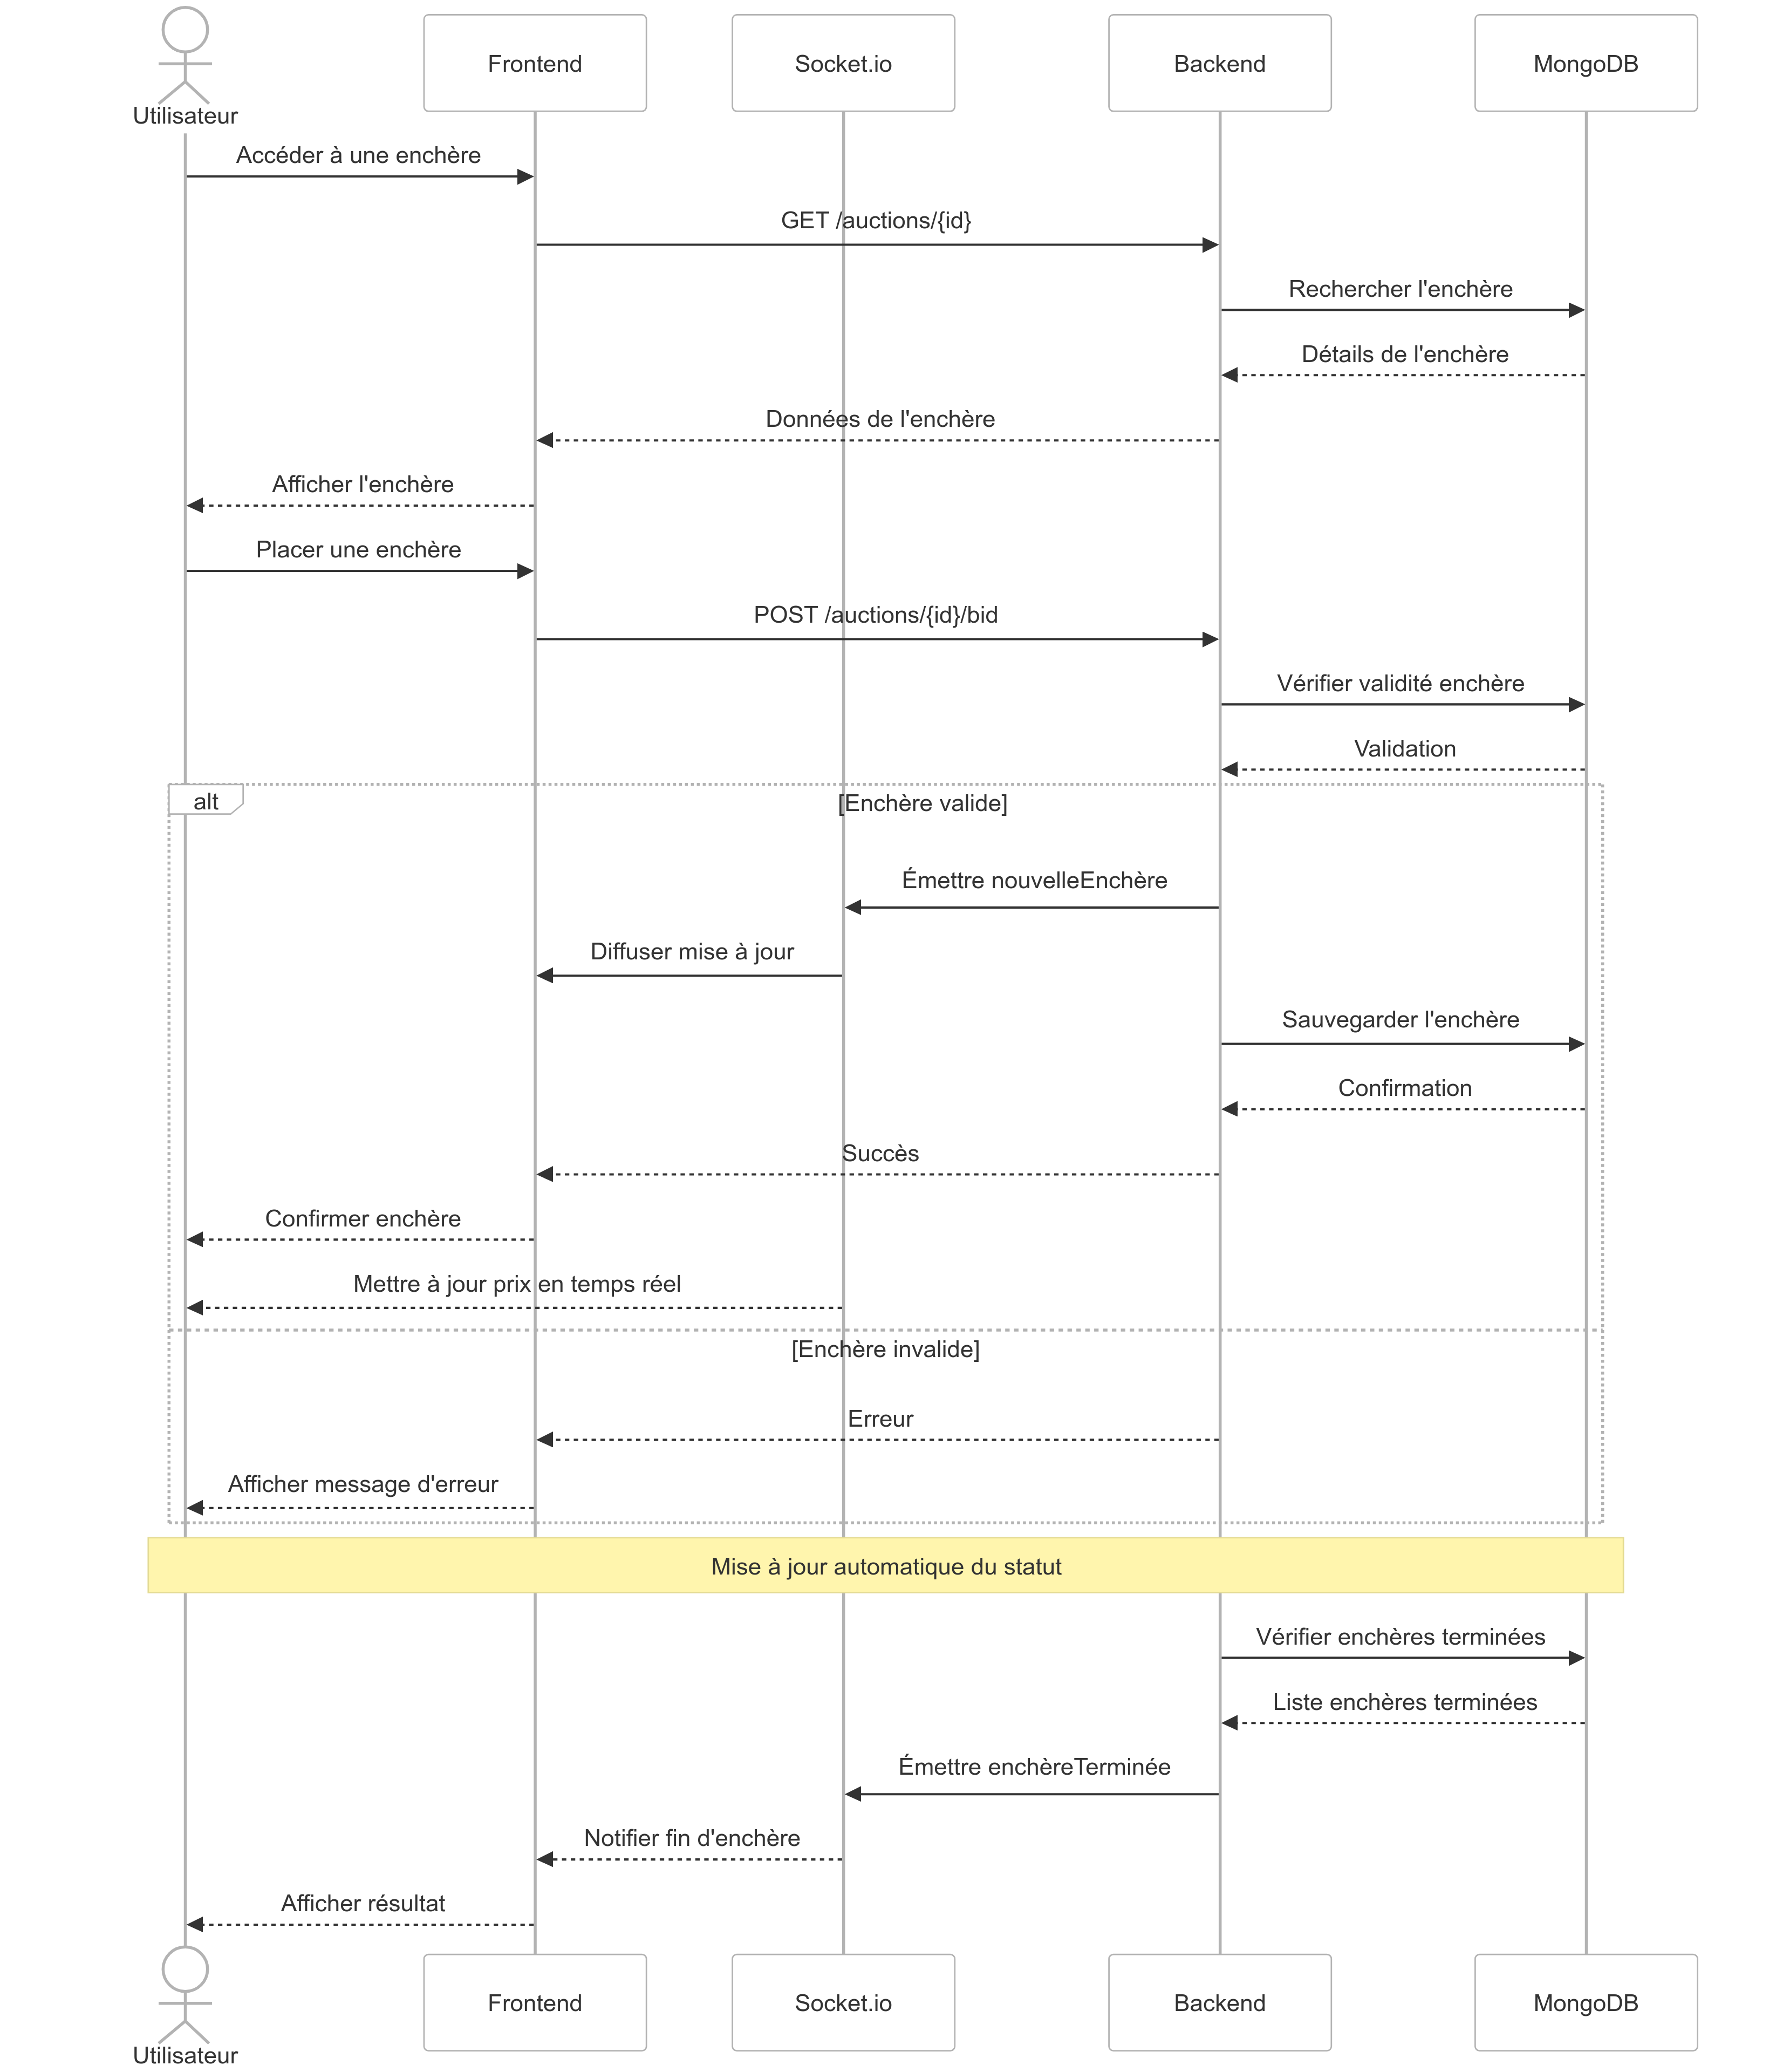
\includegraphics[width=\textwidth]{Editor _ Mermaid Chart-2025-04-03-140837.png}
    \caption{Diagramme de cas d'utilisation du système d'enchères}
    \label{fig:use-case}
\end{figure}

\subsection{Acteurs du Système}
\begin{itemize}
    \item \textbf{Utilisateur}: Représente un client qui peut consulter les enchères, s'inscrire, se connecter, placer des enchères, gérer son profil et suivre ses enchères.
    \item \textbf{Administrateur}: Dispose de privilèges étendus permettant de gérer les voitures, les utilisateurs et créer de nouvelles enchères.
\end{itemize}

\subsection{Cas d'Utilisation Principaux}
\begin{description}
    \item[Consulter les enchères] Permet aux utilisateurs de visualiser toutes les enchères actives.
    \item[S'inscrire] Création d'un nouveau compte utilisateur.
    \item[Se connecter] Authentification dans le système.
    \item[Placer une enchère] Soumettre une offre sur un véhicule en enchère.
    \item[Gérer profil] Modifier les informations personnelles.
    \item[Voir mes enchères] Consulter l'historique personnel des enchères.
    \item[Gérer les voitures] Fonctionnalité réservée à l'administrateur pour ajouter, modifier ou supprimer des véhicules.
    \item[Gérer les utilisateurs] Fonctionnalité réservée à l'administrateur pour gérer les comptes utilisateurs.
    \item[Créer une enchère] Fonctionnalité réservée à l'administrateur pour initier une nouvelle enchère.
\end{description}

\section{Diagramme de Séquence}
Le diagramme de séquence suivant illustre le flux d'interaction entre les différentes composantes du système lors du processus d'enchère.

\begin{figure}[ht]
    \centering
    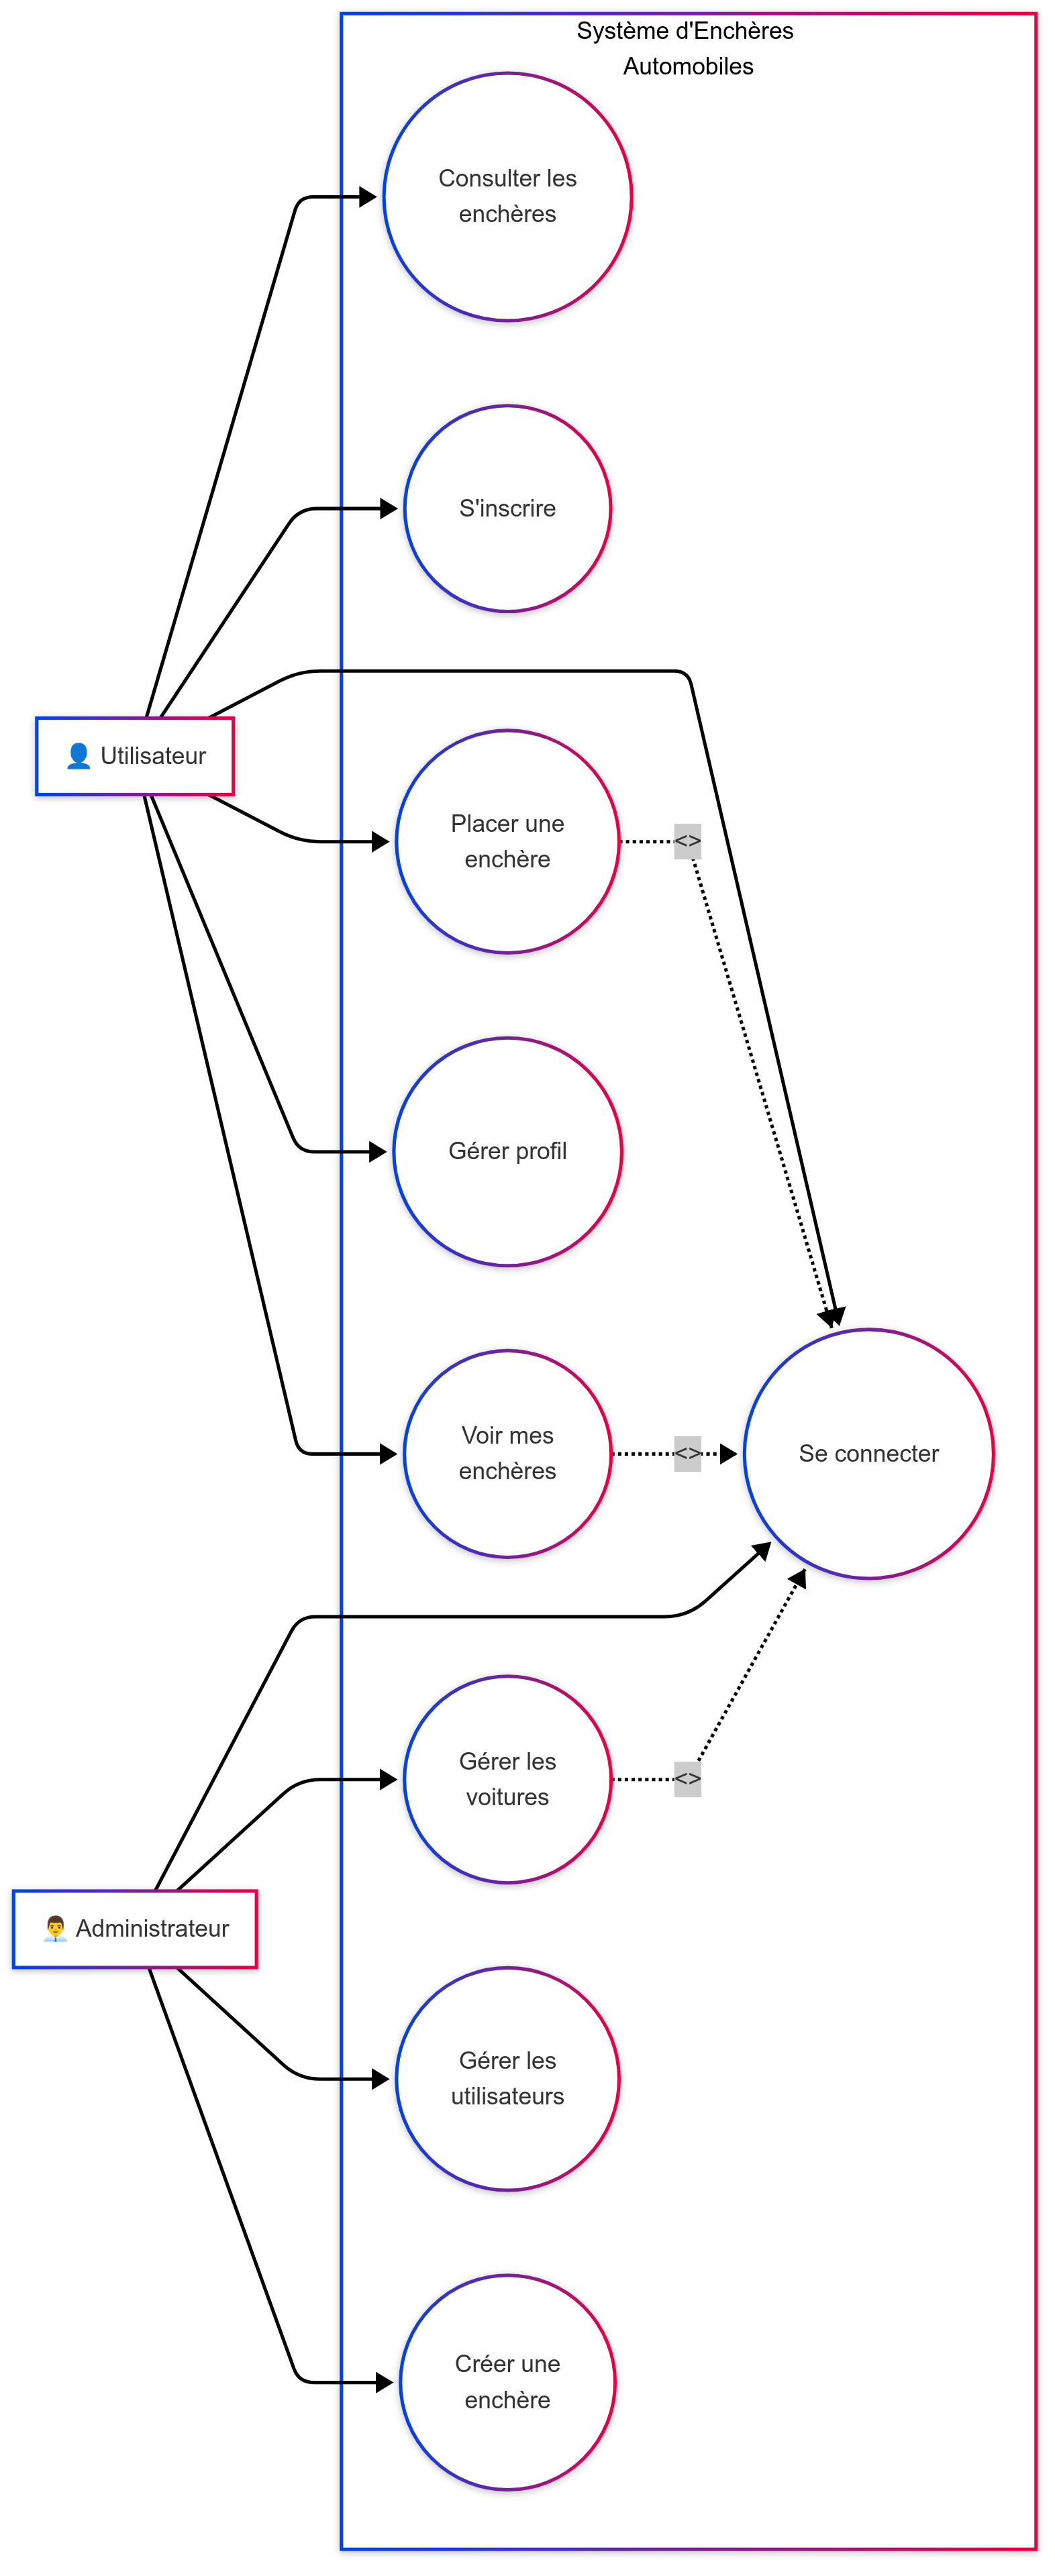
\includegraphics[width=\textwidth]{Editor _ Mermaid Chart-2025-04-03-141556.png}
    \caption{Diagramme de séquence pour le processus d'enchère}
    \label{fig:sequence-diagram}
\end{figure}

\subsection{Analyse du Flux d'Enchère}
Le diagramme de séquence décompose le processus d'enchère en plusieurs étapes clés:

\begin{enumerate}
    \item L'utilisateur accède à une enchère via l'interface frontend
    \item Le frontend demande les détails de l'enchère au backend via une requête GET
    \item Le backend interroge la base de données pour récupérer les informations
    \item L'utilisateur place une enchère qui est envoyée au serveur
    \item Le backend vérifie la validité de l'enchère
    \item Si l'enchère est valide:
    \begin{itemize}
        \item L'enchère est enregistrée dans la base de données
        \item Une notification en temps réel est émise via Socket.io
        \item Tous les clients connectés sont informés de la mise à jour
    \end{itemize}
    \item Si l'enchère est invalide, un message d'erreur est retourné
    \item Le système met à jour automatiquement le statut des enchères terminées
\end{enumerate}

\section{Diagramme de Classes}
Le diagramme de classes suivant représente la structure des entités principales du système et leurs relations.

\begin{figure}[ht]
    \centering
    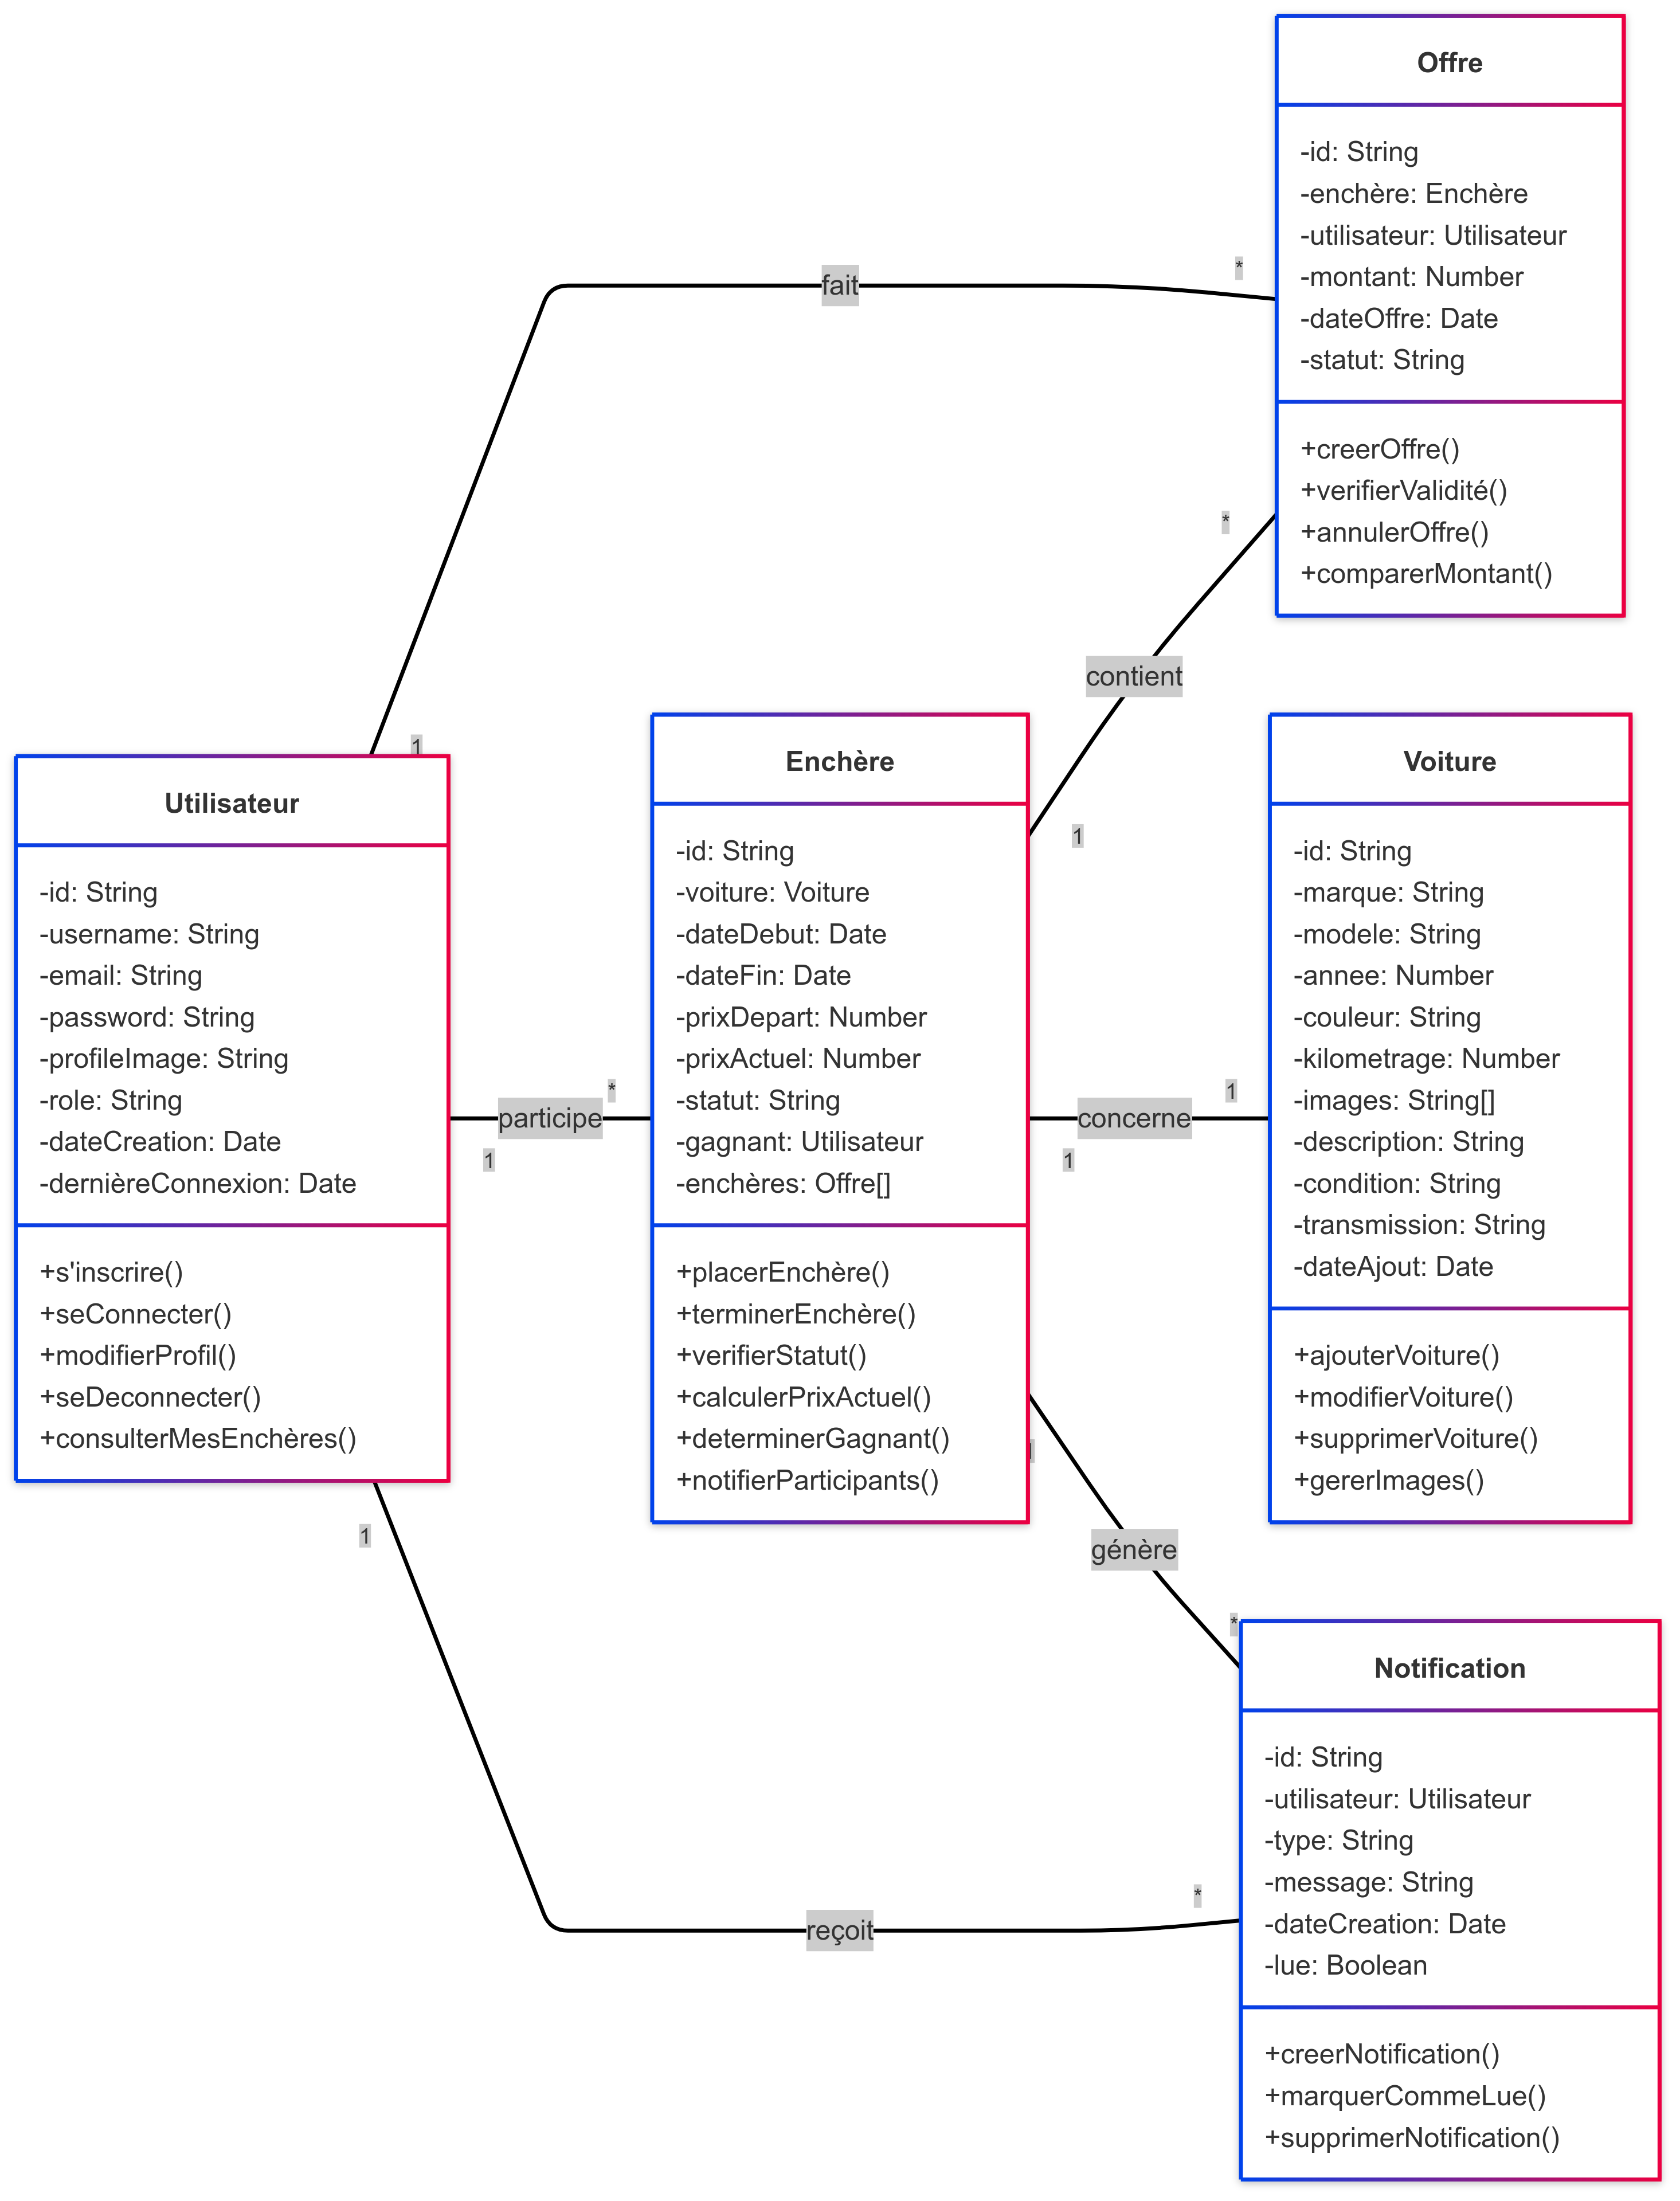
\includegraphics[width=\textwidth]{Editor _ Mermaid Chart-2025-04-03-140758.png}
    \caption{Diagramme de classes des principaux composants du système}
    \label{fig:class-diagram}
\end{figure}

\subsection{Entités Principales}
\begin{description}
    \item[Utilisateur] Contient les informations personnelles et d'authentification. Un utilisateur peut participer à plusieurs enchères et recevoir des notifications.
    \item[Enchère] Représente une session d'enchères avec une date de début, de fin, un prix de départ et un prix actuel. Une enchère concerne un véhicule spécifique et contient plusieurs offres.
    \item[Voiture] Contient les informations détaillées d'un véhicule mis aux enchères, comme la marque, le modèle, l'année, et des images.
    \item[Offre] Représente une proposition financière faite par un utilisateur dans le cadre d'une enchère.
    \item[Notification] Permet d'informer les utilisateurs des événements importants comme les surenchères ou la fin d'une enchère.
\end{description}

\subsection{Relations Entre Entités}
\begin{itemize}
    \item Un utilisateur peut participer à plusieurs enchères (relation n-n)
    \item Une enchère concerne exactement une voiture (relation 1-1)
    \item Un utilisateur peut faire plusieurs offres (relation 1-n)
    \item Une enchère contient plusieurs offres (relation 1-n)
    \item Un utilisateur reçoit plusieurs notifications (relation 1-n)
    \item Une enchère génère plusieurs notifications (relation 1-n)
\end{itemize}

\section{Modèles de Données}

\subsection{Modèle Utilisateur}
\begin{verbatim}
const userSchema = new Schema({
  id: String,
  username: String,
  email: String,
  password: String,
  profileImage: String,
  role: String,
  dateCreation: Date,
  dernièreConnexion: Date
});
\end{verbatim}

\subsection{Modèle Enchère}
\begin{verbatim}
const enchereSchema = new Schema({
  id: String,
  voiture: { type: Schema.Types.ObjectId, ref: 'Voiture' },
  dateDebut: Date,
  dateFin: Date,
  prixDepart: Number,
  prixActuel: Number,
  statut: String,
  gagnant: { type: Schema.Types.ObjectId, ref: 'Utilisateur' },
  encheres: [{ type: Schema.Types.ObjectId, ref: 'Offre' }]
});
\end{verbatim}

\subsection{Modèle Voiture}
\begin{verbatim}
const voitureSchema = new Schema({
  id: String,
  marque: String,
  modele: String,
  annee: Number,
  couleur: String,
  kilometrage: Number,
  images: [String],
  description: String,
  condition: String,
  transmission: String,
  dateAjout: Date
});
\end{verbatim}

\subsection{Modèle Offre}
\begin{verbatim}
const offreSchema = new Schema({
  id: String,
  enchere: { type: Schema.Types.ObjectId, ref: 'Enchere' },
  utilisateur: { type: Schema.Types.ObjectId, ref: 'Utilisateur' },
  montant: Number,
  dateOffre: Date,
  statut: String
});
\end{verbatim}

\section{Architecture Technique}

\subsection{Architecture Frontend}
L'application frontend est développée avec React Native, ce qui permet un déploiement sur iOS et Android à partir d'une base de code unique. Les principales composantes de l'architecture frontend sont:

\begin{itemize}
    \item \textbf{Écrans}: Représentent les différentes vues de l'application
    \item \textbf{Composants}: Éléments d'interface réutilisables
    \item \textbf{Services}: Modules pour la communication avec le backend
    \item \textbf{État global}: Gestion centralisée de l'état de l'application
    \item \textbf{Navigateurs}: Gestion de la navigation entre écrans
\end{itemize}

\subsection{Architecture Backend}
Le backend est construit sur Node.js avec Express.js comme framework web. L'architecture est organisée selon les principes MVC (Modèle-Vue-Contrôleur) adaptés aux API REST:

\begin{itemize}
    \item \textbf{Routes}: Définissent les points d'entrée API
    \item \textbf{Contrôleurs}: Contiennent la logique métier
    \item \textbf{Modèles}: Représentent les entités de base de données
    \item \textbf{Middleware}: Composants pour l'authentification et la validation
    \item \textbf{Services}: Logique partagée entre différents contrôleurs
\end{itemize}

\subsection{Communication en Temps Réel}
La communication en temps réel est gérée par Socket.io, qui permet:

\begin{itemize}
    \item Des mises à jour instantanées des enchères
    \item Des notifications en temps réel pour les utilisateurs
    \item La gestion de salles d'enchères virtuelles
    \item Une reconnexion automatique en cas de perte de connexion
\end{itemize}

\subsection{Base de Données}
MongoDB a été choisi comme système de base de données pour sa flexibilité et sa scalabilité. Les caractéristiques clés de notre implémentation MongoDB sont:

\begin{itemize}
    \item Schémas flexibles permettant une évolution rapide
    \item Relations entre documents gérées par références
    \item Indexation pour optimiser les performances de requête
    \item Agrégations pour des analyses complexes
\end{itemize}
\chapter{Réalisation Technique}

\section{Implémentation Frontend}

\subsection{Structure de l'Application Mobile}
L'application mobile représente l'interface principale par laquelle les utilisateurs interagissent avec le système d'enchères. Développée avec React Native, elle offre une expérience native sur les plateformes iOS et Android à partir d'une base de code unique.

\subsubsection{Organisation des Écrans}
L'application est structurée autour de plusieurs écrans principaux:

\begin{itemize}
    \item \textbf{AuthenticationScreen}: Gère l'inscription et la connexion des utilisateurs
    \item \textbf{AuctionListScreen}: Affiche la liste des enchères disponibles
    \item \textbf{AuctionDetailScreen}: Présente les détails d'une enchère spécifique
    \item \textbf{BiddingScreen}: Interface pour placer des enchères
    \item \textbf{ProfileScreen}: Gestion du profil utilisateur
    \item \textbf{MyAuctionsScreen}: Historique des enchères de l'utilisateur
\end{itemize}

\subsubsection{Navigation}
La navigation est gérée via React Navigation, permettant une expérience fluide entre les différents écrans:

\begin{verbatim}
const Stack = createStackNavigator();

function AppNavigator() {
  return (
    <Stack.Navigator>
      <Stack.Screen name="Home" component={HomeScreen} />
      <Stack.Screen name="AuctionDetail" component={AuctionDetailScreen} />
      <Stack.Screen name="Bidding" component={BiddingScreen} />
      <Stack.Screen name="Profile" component={ProfileScreen} />
      <Stack.Screen name="MyAuctions" component={MyAuctionsScreen} />
    </Stack.Navigator>
  );
}
\end{verbatim}

\subsection{Composants Réutilisables}
Pour maintenir la cohérence de l'interface et optimiser le développement, plusieurs composants réutilisables ont été créés:

\begin{verbatim}
// Exemple de composant réutilisable pour les enchères
const AuctionCard = ({ auction, onPress }) => (
  <TouchableOpacity 
    style={styles.card} 
    onPress={() => onPress(auction.id)}
  >
    <Image
      source={{ uri: auction.car.images[0] }}
      style={styles.carImage}
    />
    <View style={styles.infoContainer}>
      <Text style={styles.title}>
        {auction.car.brand} {auction.car.model}
      </Text>
      <Text style={styles.price}>
        Prix actuel: {auction.currentPrice} €
      </Text>
      <Text style={styles.time}>
        Fin: {formatDate(auction.endTime)}
      </Text>
    </View>
  </TouchableOpacity>
);
\end{verbatim}

\subsection{Gestion du State}
La gestion de l'état de l'application utilise les hooks React pour les composants locaux et un système centralisé pour l'état global:

\begin{verbatim}
// Exemple d'utilisation des hooks dans un écran d'enchère
function AuctionDetailScreen({ route }) {
  const { auctionId } = route.params;
  const [auction, setAuction] = useState(null);
  const [loading, setLoading] = useState(true);
  const [bidAmount, setBidAmount] = useState('');
  
  useEffect(() => {
    const fetchAuction = async () => {
      try {
        const data = await AuctionService.getAuctionById(auctionId);
        setAuction(data);
      } catch (error) {
        console.error('Error fetching auction:', error);
      } finally {
        setLoading(false);
      }
    };
    
    fetchAuction();
    
    // Configuration Socket.io pour les mises à jour en temps réel
    socket.on('auction_update', (updatedAuction) => {
      if (updatedAuction.id === auctionId) {
        setAuction(updatedAuction);
      }
    });
    
    return () => {
      socket.off('auction_update');
    };
  }, [auctionId]);
  
  // Reste de la logique du composant...
}
\end{verbatim}

\subsection{Communication Temps Réel}
L'intégration de Socket.io au frontend permet de recevoir des mises à jour en temps réel des enchères:

\begin{verbatim}
// Service Socket.io
const initializeSocket = (userId) => {
  socket = io(API_URL);
  
  socket.on('connect', () => {
    console.log('Connected to Socket.io');
    socket.emit('user_connected', { userId });
  });
  
  socket.on('new_bid', (data) => {
    // Mise à jour de l'interface en temps réel
    notifyBidUpdate(data);
  });
  
  socket.on('auction_ended', (data) => {
    // Notification de fin d'enchère
    notifyAuctionEnded(data);
  });
  
  return socket;
};
\end{verbatim}

\section{Implémentation Backend}

\subsection{Architecture API}
Le backend est implémenté en utilisant Node.js et Express.js, suivant une architecture RESTful pour exposer les points d'entrée API:

\begin{verbatim}
// Configuration principale Express
const express = require('express');
const app = express();
const http = require('http').createServer(app);
const io = require('socket.io')(http);
const mongoose = require('mongoose');
const cors = require('cors');

// Middleware
app.use(cors());
app.use(express.json());

// Routes
app.use('/api/auth', authRoutes);
app.use('/api/auctions', auctionRoutes);
app.use('/api/cars', carRoutes);
app.use('/api/users', userRoutes);

// Gestion Socket.io
io.on('connection', (socket) => {
  console.log('New client connected');
  
  socket.on('join_auction', (auctionId) => {
    socket.join(`auction_${auctionId}`);
  });
  
  socket.on('place_bid', async (data) => {
    // Traitement de l'enchère
    const result = await auctionService.placeBid(data);
    
    if (result.success) {
      io.to(`auction_${data.auctionId}`).emit('bid_update', result.data);
    }
  });
});

// Démarrage du serveur
mongoose.connect(DB_URI)
  .then(() => {
    console.log('Connected to MongoDB');
    http.listen(PORT, () => {
      console.log(`Server running on port ${PORT}`);
    });
  });
\end{verbatim}

\subsection{Contrôleurs}
Les contrôleurs implémentent la logique métier principale:

\begin{verbatim}
// Contrôleur d'enchères
const auctionController = {
  // Récupérer toutes les enchères actives
  getAllActive: async (req, res) => {
    try {
      const auctions = await Auction.find({ status: 'active' })
        .populate('car')
        .sort({ endTime: 1 });
      
      res.json(auctions);
    } catch (error) {
      res.status(500).json({ message: error.message });
    }
  },
  
  // Récupérer une enchère par son ID
  getById: async (req, res) => {
    try {
      const auction = await Auction.findById(req.params.id)
        .populate('car')
        .populate({
          path: 'bids',
          populate: { path: 'user', select: 'username' }
        });
      
      if (!auction) {
        return res.status(404).json({ message: 'Enchère non trouvée' });
      }
      
      res.json(auction);
    } catch (error) {
      res.status(500).json({ message: error.message });
    }
  },
  
  // Placer une enchère
  placeBid: async (req, res) => {
    try {
      const { auctionId, amount } = req.body;
      const userId = req.user.id;
      
      const result = await auctionService.placeBid({
        auctionId,
        userId,
        amount
      });
      
      if (result.success) {
        res.json(result.data);
      } else {
        res.status(400).json({ message: result.message });
      }
    } catch (error) {
      res.status(500).json({ message: error.message });
    }
  }
};
\end{verbatim}

\subsection{Middleware}
Les middleware gèrent l'authentification et la validation:

\begin{verbatim}
// Middleware d'authentification
const authMiddleware = async (req, res, next) => {
  try {
    const token = req.header('Authorization').replace('Bearer ', '');
    const decoded = jwt.verify(token, JWT_SECRET);
    const user = await User.findById(decoded.id);
    
    if (!user) {
      throw new Error();
    }
    
    req.token = token;
    req.user = user;
    next();
  } catch (error) {
    res.status(401).json({ message: 'Veuillez vous authentifier' });
  }
};
\end{verbatim}

\subsection{Services}
Les services encapsulent la logique réutilisable entre différents contrôleurs:

\begin{verbatim}
// Service d'enchères
const auctionService = {
  // Placer une enchère
  placeBid: async ({ auctionId, userId, amount }) => {
    // Validation des entrées
    if (!mongoose.Types.ObjectId.isValid(auctionId)) {
      return { success: false, message: 'ID d\'enchère invalide' };
    }
    
    const amountNum = parseFloat(amount);
    if (isNaN(amountNum)) {
      return { success: false, message: 'Montant invalide' };
    }
    
    // Début de transaction
    const session = await mongoose.startSession();
    session.startTransaction();
    
    try {
      // Récupérer l'enchère avec verrouillage
      const auction = await Auction.findById(auctionId).session(session);
      
      if (!auction) {
        throw new Error('Enchère non trouvée');
      }
      
      if (auction.status !== 'active') {
        throw new Error('L\'enchère n\'est plus active');
      }
      
      if (auction.endTime < new Date()) {
        throw new Error('L\'enchère est terminée');
      }
      
      if (amountNum <= auction.currentPrice) {
        throw new Error('Le montant doit être supérieur au prix actuel');
      }
      
      // Créer la nouvelle enchère
      const bid = new Bid({
        auction: auctionId,
        user: userId,
        amount: amountNum,
        createdAt: new Date()
      });
      
      await bid.save({ session });
      
      // Mettre à jour l'enchère
      auction.currentPrice = amountNum;
      auction.bids.push(bid._id);
      await auction.save({ session });
      
      // Valider la transaction
      await session.commitTransaction();
      
      // Populer les données pour la réponse
      const populatedBid = await Bid.findById(bid._id)
        .populate('user', 'username')
        .lean();
      
      return {
        success: true,
        data: {
          bid: populatedBid,
          newPrice: amountNum,
          auctionId
        }
      };
    } catch (error) {
      // Annuler la transaction en cas d'erreur
      await session.abortTransaction();
      return { success: false, message: error.message };
    } finally {
      session.endSession();
    }
  },
  
  // Vérifier et mettre à jour les enchères terminées
  checkEndedAuctions: async () => {
    const now = new Date();
    
    const endedAuctions = await Auction.find({
      status: 'active',
      endTime: { $lte: now }
    });
    
    for (const auction of endedAuctions) {
      // Trouver le gagnant
      if (auction.bids.length > 0) {
        const highestBid = await Bid.findOne({ auction: auction._id })
          .sort({ amount: -1 })
          .populate('user');
        
        if (highestBid) {
          auction.winner = highestBid.user._id;
        }
      }
      
      auction.status = 'ended';
      await auction.save();
      
      // Émettre un événement de fin d'enchère
      io.to(`auction_${auction._id}`).emit('auction_ended', {
        auctionId: auction._id,
        winner: auction.winner
      });
    }
    
    return endedAuctions;
  }
};
\end{verbatim}

\section{Intégration et Tests}

\subsection{Tests Unitaires}
Les tests unitaires couvrent les fonctionnalités critiques du système:

\begin{verbatim}
// Test du service d'enchères
describe('Auction Service Tests', () => {
  test('Devrait rejeter une enchère inférieure au prix actuel', async () => {
    // Configuration du test
    const auctionId = new mongoose.Types.ObjectId();
    const userId = new mongoose.Types.ObjectId();
    
    // Mock de l'enchère
    jest.spyOn(Auction, 'findById').mockResolvedValue({
      _id: auctionId,
      currentPrice: 1000,
      status: 'active',
      endTime: new Date(Date.now() + 3600000), // +1 heure
      bids: [],
      save: jest.fn().mockResolvedValue(true)
    });
    
    // Exécution du test
    const result = await auctionService.placeBid({
      auctionId,
      userId,
      amount: 900 // Inférieur au prix actuel
    });
    
    // Vérification des résultats
    expect(result.success).toBe(false);
    expect(result.message).toContain('supérieur au prix actuel');
  });
});
\end{verbatim}

\subsection{Déploiement}
L'application est déployée à l'aide d'une infrastructure cloud garantissant haute disponibilité et scalabilité:

\begin{itemize}
    \item \textbf{Frontend}: Déployé via les app stores (Google Play et App Store)
    \item \textbf{Backend}: Conteneurisé avec Docker et déployé sur une plateforme Kubernetes
    \item \textbf{Base de données}: MongoDB Atlas pour une solution gérée et scalable
    \item \textbf{Monitoring}: Intégration de solutions de monitoring pour surveiller les performances et la disponibilité
\end{itemize}

\subsection{Sécurité}
Plusieurs mesures de sécurité ont été implémentées:

\begin{itemize}
    \item Stockage sécurisé des mots de passe avec bcrypt
    \item Protection contre les attaques par injection via la validation des entrées
    \item Authentification basée sur les tokens JWT
    \item Gestion sécurisée des sessions
    \item Protection contre les attaques CSRF
    \item Configuration HTTPS pour toutes les communications
\end{itemize}

\section{Défis Techniques et Solutions}

\subsection{Concurrence dans les Enchères}
Un défi majeur était de gérer la concurrence lorsque plusieurs utilisateurs placent des enchères simultanément:

\begin{itemize}
    \item \textbf{Problème}: Risque de conditions de course (race conditions) entraînant des incohérences dans les données.
    \item \textbf{Solution}: Utilisation de transactions MongoDB avec verrouillage optimiste pour garantir l'intégrité des données.
\end{itemize}

\subsection{Performances en Temps Réel}
Le maintien des performances pour un grand nombre d'utilisateurs simultanés était essentiel:

\begin{itemize}
    \item \textbf{Problème}: Surcharge potentielle du serveur lors de pics d'activité.
    \item \textbf{Solution}: 
    \begin{itemize}
        \item Optimisation de l'architecture Socket.io avec des espaces de noms et des salles
        \item Mise en cache des données fréquemment accédées
        \item Architecture horizontalement scalable
    \end{itemize}
\end{itemize}

\subsection{Gestion des Images}
La gestion efficace des images de véhicules représentait un défi important:

\begin{itemize}
    \item \textbf{Problème}: Stockage et livraison optimisés des images des véhicules.
    \item \textbf{Solution}: 
    \begin{itemize}
        \item Utilisation d'un CDN pour la distribution des images
        \item Redimensionnement automatique des images en fonction du contexte d'affichage
        \item Compression progressive pour améliorer la vitesse de chargement
    \end{itemize}
\end{itemize} 
\chapter{Défis d'Implémentation et Perspectives d'Évolution}

\section{Défis Techniques Rencontrés}

\subsection{Gestion de la Concurrence}
Un des défis majeurs dans le développement de cette application d'enchères a été la gestion de la concurrence. Les enchères étant un environnement où plusieurs utilisateurs peuvent agir simultanément sur les mêmes ressources, nous avons dû mettre en place des mécanismes solides pour éviter les conflits et garantir l'intégrité des données.

\subsubsection{Problématique}
Les problèmes spécifiques liés à la concurrence incluaient:
\begin{itemize}
    \item Risque de conditions de course lors de la mise à jour du prix actuel d'une enchère
    \item Possibilité d'enchères soumises après la date de fin
    \item Conflit potentiel lors de la détermination du gagnant si plusieurs offres arrivent simultanément
\end{itemize}

\subsubsection{Solutions Implémentées}
Pour résoudre ces problèmes, nous avons mis en œuvre:
\begin{itemize}
    \item Une architecture basée sur les transactions MongoDB, garantissant l'atomicité des opérations
    \item Un mécanisme de verrouillage optimiste pour prévenir les mises à jour simultanées contradictoires
    \item Une validation côté serveur systématique avec horodatage précis pour les enchères
    \item Un système de file d'attente pour traiter les enchères dans l'ordre chronologique
\end{itemize}

\begin{verbatim}
// Exemple de gestion de transaction pour placer une enchère
const placeBid = async (auctionId, userId, amount) => {
  const session = await mongoose.startSession();
  session.startTransaction();
  
  try {
    // Verrouillage optimiste avec version
    const auction = await Auction.findById(auctionId).session(session);
    if (!auction) throw new Error('Enchère non trouvée');
    
    // Vérifications de validité
    if (auction.status !== 'active') throw new Error('Enchère non active');
    if (auction.endTime < new Date()) throw new Error('Enchère terminée');
    if (amount <= auction.currentPrice) throw new Error('Montant insuffisant');
    
    // Création de l'offre et mise à jour de l'enchère
    const bid = new Bid({ auction: auctionId, user: userId, amount });
    await bid.save({ session });
    
    auction.currentPrice = amount;
    auction.bids.push(bid._id);
    await auction.save({ session });
    
    await session.commitTransaction();
    return { success: true, bid };
  } catch (error) {
    await session.abortTransaction();
    return { success: false, error: error.message };
  } finally {
    session.endSession();
  }
};
\end{verbatim}

\subsection{Optimisation des Performances}
La nature temps réel de l'application exigeait une attention particulière aux performances, surtout pendant les périodes de forte activité.

\subsubsection{Problématique}
Les défis de performance incluaient:
\begin{itemize}
    \item Latence potentielle lors de la mise à jour en temps réel des prix d'enchères
    \item Surcharge du serveur pendant les dernières minutes d'une enchère populaire
    \item Gestion efficace d'un grand nombre de connexions simultanées
    \item Temps de réponse de la base de données sous charge élevée
\end{itemize}

\subsubsection{Solutions Implémentées}
Pour optimiser les performances, nous avons:
\begin{itemize}
    \item Implémenté une architecture basée sur des microservices pour une meilleure scalabilité horizontale
    \item Utilisé Redis comme solution de cache pour réduire la charge sur MongoDB
    \item Optimisé les requêtes MongoDB avec des index appropriés
    \item Implémenté un système de limitation de débit (rate limiting) pour éviter les surcharges
    \item Configuré Socket.io avec des espaces de noms et des salles pour optimiser la diffusion des messages
\end{itemize}

\begin{verbatim}
// Configuration Socket.io avec espaces de noms et salles
const io = require('socket.io')(server);
const auctionNamespace = io.of('/auctions');

auctionNamespace.on('connection', (socket) => {
  // Rejoindre des salles spécifiques pour les enchères
  socket.on('join_auction', (auctionId) => {
    socket.join(`auction_${auctionId}`);
  });
  
  // Diffusion ciblée aux participants d'une enchère spécifique
  socket.on('place_bid', async (data) => {
    const result = await auctionService.placeBid(data);
    if (result.success) {
      auctionNamespace.to(`auction_${data.auctionId}`).emit('bid_update', result.data);
    } else {
      socket.emit('bid_error', { message: result.error });
    }
  });
});
\end{verbatim}

\subsection{Sécurité et Authentification}
La sécurité était une priorité absolue pour protéger les données des utilisateurs et maintenir l'intégrité des enchères.

\subsubsection{Problématique}
Les défis de sécurité incluaient:
\begin{itemize}
    \item Protection contre les attaques par force brute
    \item Risque de manipulation des enchères par des utilisateurs malveillants
    \item Sécurisation des communications en temps réel
    \item Protection des données sensibles des utilisateurs
\end{itemize}

\subsubsection{Solutions Implémentées}
Pour renforcer la sécurité, nous avons:
\begin{itemize}
    \item Implémenté un système d'authentification robuste basé sur JWT avec rotation des tokens
    \item Mis en place une validation stricte des entrées côté serveur
    \item Configuré HTTPS pour toutes les communications
    \item Appliqué des politiques de mot de passe fort avec hachage bcrypt
    \item Implémenté une détection d'activité suspecte avec blocage temporaire des comptes
    \item Sécurisé les connexions WebSocket avec des tokens d'authentification
\end{itemize}

\begin{verbatim}
// Middleware d'authentification pour Socket.io
const authenticateSocket = (socket, next) => {
  const token = socket.handshake.auth.token;
  if (!token) {
    return next(new Error('Authentication error'));
  }
  
  try {
    const decoded = jwt.verify(token, JWT_SECRET);
    socket.user = decoded;
    next();
  } catch (error) {
    next(new Error('Invalid token'));
  }
};

io.use(authenticateSocket);
\end{verbatim}

\section{Perspectives d'Évolution}

\subsection{Fonctionnalités Additionnelles}
Sur la base du système actuel, plusieurs fonctionnalités pourraient être ajoutées pour enrichir l'expérience utilisateur:

\subsubsection{Système de Paiement Intégré}
L'intégration d'une solution de paiement permettrait de finaliser les transactions directement dans l'application:
\begin{itemize}
    \item Intégration avec des API de paiement populaires (Stripe, PayPal)
    \item Gestion de dépôts de garantie pour les enchères
    \item Système de facturation automatisé
    \item Suivi des transactions et historique des paiements
\end{itemize}

\subsubsection{Système de Notation et d'Avis}
Un système permettant aux utilisateurs d'évaluer les vendeurs et les véhicules après achat:
\begin{itemize}
    \item Notations et commentaires sur les vendeurs
    \item Vérification de l'authenticité des avis
    \item Impact sur la réputation et la visibilité des vendeurs
    \item Système de badges pour les vendeurs fiables
\end{itemize}

\subsubsection{Assistant d'Enchères Intelligent}
Un assistant basé sur l'IA pour aider les utilisateurs dans leur stratégie d'enchères:
\begin{itemize}
    \item Prédiction des tendances de prix basée sur l'historique
    \item Recommandations personnalisées de véhicules
    \item Aide à la décision pour le montant optimal des enchères
    \item Alertes intelligentes pour les opportunités d'enchères
\end{itemize}

\subsubsection{Système de Messagerie Interne}
Une plateforme de communication directe entre acheteurs et vendeurs:
\begin{itemize}
    \item Messagerie privée sécurisée
    \item Possibilité de poser des questions sur les véhicules
    \item Négociation post-enchère
    \item Partage sécurisé de documents
\end{itemize}

\subsection{Améliorations Techniques}

\subsubsection{Architecture Serverless}
Migration vers une architecture serverless pour améliorer la scalabilité et réduire les coûts:
\begin{itemize}
    \item Utilisation de AWS Lambda ou Azure Functions pour le backend
    \item API Gateway pour la gestion des requêtes
    \item WebSockets managés avec des services cloud
    \item Base de données distribuée pour une meilleure résilience
\end{itemize}

\subsubsection{Progressive Web App (PWA)}
Transformation de l'application en PWA pour améliorer l'accessibilité:
\begin{itemize}
    \item Fonctionnalités hors ligne avec synchronisation
    \item Installation sur l'écran d'accueil sans passer par les app stores
    \item Push notifications pour les mises à jour d'enchères
    \item Expérience utilisateur améliorée sur tous les appareils
\end{itemize}

\subsubsection{Intelligence Artificielle et Machine Learning}
Intégration de fonctionnalités IA pour enrichir l'application:
\begin{itemize}
    \item Estimation automatique de la valeur des véhicules
    \item Détection de fraude et d'activités suspectes
    \item Optimisation dynamique des prix de départ basée sur des données historiques
    \item Recommandations personnalisées basées sur le comportement des utilisateurs
\end{itemize}

\subsection{Expansion Internationale}

\subsubsection{Multilinguisme et Localisation}
Pour atteindre un public international:
\begin{itemize}
    \item Support de multiples langues dans l'interface
    \item Adaptation aux différentes devises et formats régionaux
    \item Conformité aux réglementations locales sur les enchères
    \item Personnalisation des contenus selon les marchés cibles
\end{itemize}

\subsubsection{Infrastructure Géo-Distribuée}
Pour offrir une latence minimale aux utilisateurs du monde entier:
\begin{itemize}
    \item Déploiement multi-régional des serveurs
    \item Réseau de diffusion de contenu (CDN) pour les ressources statiques
    \item Réplication géographique des bases de données
    \item Monitoring et métriques par région
\end{itemize}

\section{Analyse Comparative avec des Solutions Existantes}

\subsection{Forces du Système}
Par rapport aux plateformes d'enchères automobile existantes, notre solution présente plusieurs avantages:
\begin{itemize}
    \item Interface utilisateur intuitive et moderne
    \item Système de notification en temps réel plus réactif
    \item Architecture technique plus flexible et évolutive
    \item Optimisation pour les appareils mobiles
    \item Meilleure intégration des fonctionnalités sociales
\end{itemize}

\subsection{Opportunités d'Amélioration}
Des domaines où notre système pourrait s'améliorer:
\begin{itemize}
    \item Enrichir les fonctionnalités de vérification des véhicules
    \item Développer des partenariats avec des services d'inspection
    \item Renforcer les outils d'analyse de marché
    \item Améliorer les fonctionnalités pour les vendeurs professionnels
\end{itemize}

\section{Impact Écologique et Économique}

\subsection{Réduction de l'Empreinte Carbone}
L'application peut contribuer positivement à l'environnement:
\begin{itemize}
    \item Réduction des déplacements pour voir des véhicules grâce aux informations détaillées
    \item Optimisation de la réutilisation des véhicules d'occasion
    \item Possibilité de promotion des véhicules électriques et hybrides
\end{itemize}

\subsection{Démocratisation du Marché Automobile}
Impact économique positif:
\begin{itemize}
    \item Accès facilité au marché pour les petits vendeurs
    \item Transparence des prix favorisant une concurrence équitable
    \item Réduction des intermédiaires et des coûts associés
    \item Potentiel de création d'emplois dans le secteur des services automobiles associés
\end{itemize} 
\chapter{Conclusion}

\section{Synthèse du Projet}

Le développement du système d'enchères automobiles a représenté un défi technique significatif, nécessitant une approche méthodique et une architecture robuste pour répondre aux exigences de performance, sécurité et expérience utilisateur. Ce projet a permis de mettre en œuvre des solutions innovantes pour résoudre des problématiques complexes liées aux applications en temps réel.

\subsection{Réalisations Principales}

Le système développé se distingue par plusieurs aspects notables:

\begin{itemize}
    \item Une architecture complète client-serveur utilisant des technologies modernes (React Native, Node.js, MongoDB, Socket.io)
    \item Un système d'enchères en temps réel performant et fiable, gérant efficacement la concurrence
    \item Une interface utilisateur intuitive et réactive sur plateformes mobiles
    \item Un backend sécurisé avec une gestion robuste de l'authentification et des autorisations
    \item Une conception évolutive permettant l'ajout futur de fonctionnalités
\end{itemize}

\subsection{Objectifs Atteints}

Le projet a répondu avec succès aux objectifs initiaux:

\begin{itemize}
    \item Permettre aux utilisateurs de participer facilement à des enchères automobiles depuis leurs appareils mobiles
    \item Garantir l'équité et la transparence du processus d'enchère
    \item Fournir une expérience utilisateur fluide et engageante
    \item Assurer la sécurité des données et des transactions
    \item Offrir une plateforme adaptable aux évolutions du marché
\end{itemize}

\section{Compétences Développées}

La réalisation de ce projet a permis de développer et d'approfondir plusieurs compétences techniques et organisationnelles:

\subsection{Compétences Techniques}

\begin{itemize}
    \item Maîtrise du développement d'applications mobiles avec React Native
    \item Conception et implémentation d'API RESTful avec Node.js et Express
    \item Gestion efficace des communications en temps réel avec Socket.io
    \item Modélisation et optimisation de bases de données NoSQL (MongoDB)
    \item Mise en œuvre de mécanismes d'authentification et de sécurité avancés
    \item Déploiement et maintenance d'applications sur infrastructures cloud
\end{itemize}

\subsection{Compétences Méthodologiques}

\begin{itemize}
    \item Application des principes de conception UML pour modéliser le système
    \item Gestion de projet agile permettant une adaptation continue aux besoins
    \item Tests et assurance qualité systématiques
    \item Documentation approfondie du code et de l'architecture
    \item Analyse et résolution de problèmes complexes
\end{itemize}

\section{Apports Personnels et Professionnels}

Ce projet a constitué une expérience enrichissante tant sur le plan personnel que professionnel:

\subsection{Développement Personnel}

\begin{itemize}
    \item Renforcement des capacités d'analyse et de résolution de problèmes
    \item Amélioration des compétences en gestion du temps et des priorités
    \item Développement de la persévérance face aux obstacles techniques
    \item Perfectionnement de l'autonomie dans l'apprentissage de nouvelles technologies
\end{itemize}

\subsection{Développement Professionnel}

\begin{itemize}
    \item Acquisition d'une expérience pratique avec des technologies de pointe
    \item Compréhension approfondie des enjeux de développement d'applications commerciales
    \item Constitution d'un portfolio démontrant des compétences diversifiées
    \item Préparation aux défis du marché du travail dans le développement d'applications
\end{itemize}

\section{Perspectives d'Avenir}

\subsection{Évolution du Projet}

Le système d'enchères automobiles dispose d'un potentiel d'évolution important:

\begin{itemize}
    \item Intégration de fonctionnalités basées sur l'intelligence artificielle pour l'estimation des valeurs de véhicules et les recommandations personnalisées
    \item Expansion vers une marketplace complète incluant services et pièces automobiles
    \item Développement d'une version web progressive en complément des applications mobiles
    \item Internationalisation pour atteindre des marchés globaux
\end{itemize}

\subsection{Applications des Connaissances Acquises}

Les compétences et connaissances acquises durant ce projet peuvent être appliquées à divers domaines:

\begin{itemize}
    \item Développement d'autres applications de commerce électronique en temps réel
    \item Conception de systèmes financiers nécessitant intégrité et performance
    \item Création de plateformes collaboratives avec interactions en temps réel
    \item Implémentation de solutions de communication sécurisées
\end{itemize}

\section{Mot de Fin}

La réalisation de ce système d'enchères automobiles représente une étape significative dans notre parcours professionnel. Au-delà des aspects techniques, ce projet nous a permis de comprendre l'importance de concevoir des solutions centrées sur l'utilisateur, robustes techniquement et évolutives pour s'adapter aux besoins futurs.

Les défis rencontrés et surmontés tout au long du développement ont renforcé notre confiance en notre capacité à aborder des problèmes complexes, à rechercher et implémenter des solutions innovantes, et à livrer des produits de qualité.

Nous sommes convaincus que les connaissances et l'expérience acquises constitueront une base solide pour nos futurs projets et contribueront significativement à notre évolution professionnelle dans le domaine du développement d'applications. 
\chapter{Annexes}

\section{Guide d'Installation}
\subsection{Prérequis}
\begin{itemize}
    \item Node.js v23.10.0 ou supérieur
    \item MongoDB
    \item Xcode (pour iOS)
    \item npm ou yarn
\end{itemize}

\subsection{Installation du Projet}
\begin{lstlisting}[language=bash]
# Clone du projet
git clone [URL_DU_PROJET]

# Installation des dépendances backend
cd backend
npm install

# Installation des dépendances frontend admin
cd ../admin-dashboard
npm install

# Installation des dépendances mobile
cd ../mobile
npm install
\end{lstlisting}

\subsection{Configuration}
\begin{lstlisting}[language=bash]
# Configuration des ports
Backend: 5001
Admin Dashboard: 3000
Metro Bundler: 8081

# En cas de conflit de ports
lsof -ti:5001,3000,8081 | xargs kill -9
\end{lstlisting}

\section{Documentation API}
\subsection{Routes d'Authentification}
\begin{itemize}
    \item \textbf{POST /api/auth/register}
    \begin{lstlisting}[language=JavaScript]
    {
        "email": "string",
        "password": "string",
        "name": "string"
    }
    \end{lstlisting}
    
    \item \textbf{POST /api/auth/login}
    \begin{lstlisting}[language=JavaScript]
    {
        "email": "string",
        "password": "string"
    }
    \end{lstlisting}
\end{itemize}

\subsection{Routes des Enchères}
\begin{itemize}
    \item \textbf{GET /api/auctions}
    \item \textbf{POST /api/auctions}
    \begin{lstlisting}[language=JavaScript]
    {
        "title": "string",
        "description": "string",
        "startPrice": "number",
        "startTime": "date",
        "endTime": "date"
    }
    \end{lstlisting}
    
    \item \textbf{POST /api/auctions/:id/bid}
    \begin{lstlisting}[language=JavaScript]
    {
        "amount": "number"
    }
    \end{lstlisting}
\end{itemize}

\section{Schéma de la Base de Données}
\subsection{Collection Users}
\begin{lstlisting}[language=JavaScript]
{
    "_id": ObjectId,
    "email": String,
    "password": String,
    "name": String,
    "role": String,
    "createdAt": Date
}
\end{lstlisting}

\subsection{Collection Auctions}
\begin{lstlisting}[language=JavaScript]
{
    "_id": ObjectId,
    "title": String,
    "description": String,
    "startPrice": Number,
    "currentPrice": Number,
    "startTime": Date,
    "endTime": Date,
    "status": String,
    "winner": ObjectId,
    "bids": Array
}
\end{lstlisting}

% Appendice : Images de l'application
\section{Captures d'écran de l'application}

% Images commented out due to missing files
%\begin{figure}[h]
%\centering
%\includegraphics[width=0.4\textwidth]{images/app_screenshot1.png}
%\caption{Écran principal de l'application mobile}
%\label{fig:app_screenshot}
%\end{figure}

%\begin{figure}[h]
%\centering
%\includegraphics[width=0.8\textwidth]{images/admin_dashboard.png}
%\caption{Tableau de bord administrateur}
%\label{fig:admin_dashboard}
%\end{figure}

\section{Logs et Débogage}
\subsection{Exemple de Logs}
\begin{lstlisting}[language=bash]
# Logs de mise à jour des statuts
Status updates: 0 became active, 0 ended
Processed winners for 2 newly ended auctions

# Logs de démarrage du serveur
Upload directories created successfully
Server running on port 5001
Connected to MongoDB
\end{lstlisting}

\section{Scripts Utiles}
\subsection{Gestion des Processus}
\begin{lstlisting}[language=bash]
# Démarrage du backend
cd backend && npm start

# Démarrage du dashboard admin
cd admin-dashboard && npm start

# Démarrage du bundler React Native
npx react-native start --reset-cache

# Lancement de l'app iOS
npx react-native run-ios
\end{lstlisting} 

% Print bibliography
\printbibliography[heading=bibintoc, title={Bibliographie}]

\end{document} 